%% abtex2-modelo-include-comandos.tex, v-1.9.5 laurocesar
%% Copyright 2012-2015 by abnTeX2 group at http://www.abntex.net.br/ 
%%
%% This work may be distributed and/or modified under the
%% conditions of the LaTeX Project Public License, either version 1.3
%% of this license or (at your option) any later version.
%% The latest version of this license is in
%%   http://www.latex-project.org/lppl.txt
%% and version 1.3 or later is part of all distributions of LaTeX
%% version 2005/12/01 or later.
%%
%% This work has the LPPL maintenance status `maintained'.
%% 
%% The Current Maintainer of this work is the abnTeX2 team, led
%% by Lauro César Araujo. Further information are available on 
%% http://www.abntex.net.br/
%%
%% This work consists of the files abntex2-modelo-include-comandos.tex
%% and abntex2-modelo-img-marca.pdf
%%

% ---
% Este capítulo, utilizado por diferentes exemplos do abnTeX2, ilustra o uso de
% comandos do abnTeX2 e de LaTeX.
% ---


 

\chapter{Fundamentação Teórica}\label{cap_fundamentacao}

A presente Seção tem por objetivo elencar a relação de trabalhos correlatos obtidos por meio de Revisão Sistemática da Literatura além de documentar conceitos fundamentais referentes ao funcionamento dos Sistemas de Detecção de Intrusão, às técnicas de \textit{Machine Learning}, conceitos acerca dos \textit{datasets} e demais informações que possam ser úteis para compreensão da proposta apresentada no âmbito desta Dissertação de Mestrado.


\section{Revisão Sistemática da Literatura}
\label{rev_sistematica}

A Revisão Sistemática da Literatura consiste em realizar o levantamento de trabalhos correlatos de forma com que o processo possa ser replicável por terceiros. \citeonline{kitchenham2007guidelines} destacam a importância da definição dos critérios de busca para que haja uma prospecção criteriosa em relação aos artigos que serão selecionados, além de que, como já citado, o método de coleta seja reproduzível por outros pesquisadores. \citeonline{biolchini2005systematic} descreve o procedimento como sendo uma forma de se obter evidência na literatura que possam justificar a própria pesquisa e que deve ser realizada após a definição de um protocolo de buscas e de um processo geral. A Figura \ref{fig:processo_rev_sistematica} ilustra o procedimento usado nesta pesquisa:

\begin{figure}[H]
\centering
\caption{Procedimento adotado para realização da Revisão Sistemática da Literatura.} 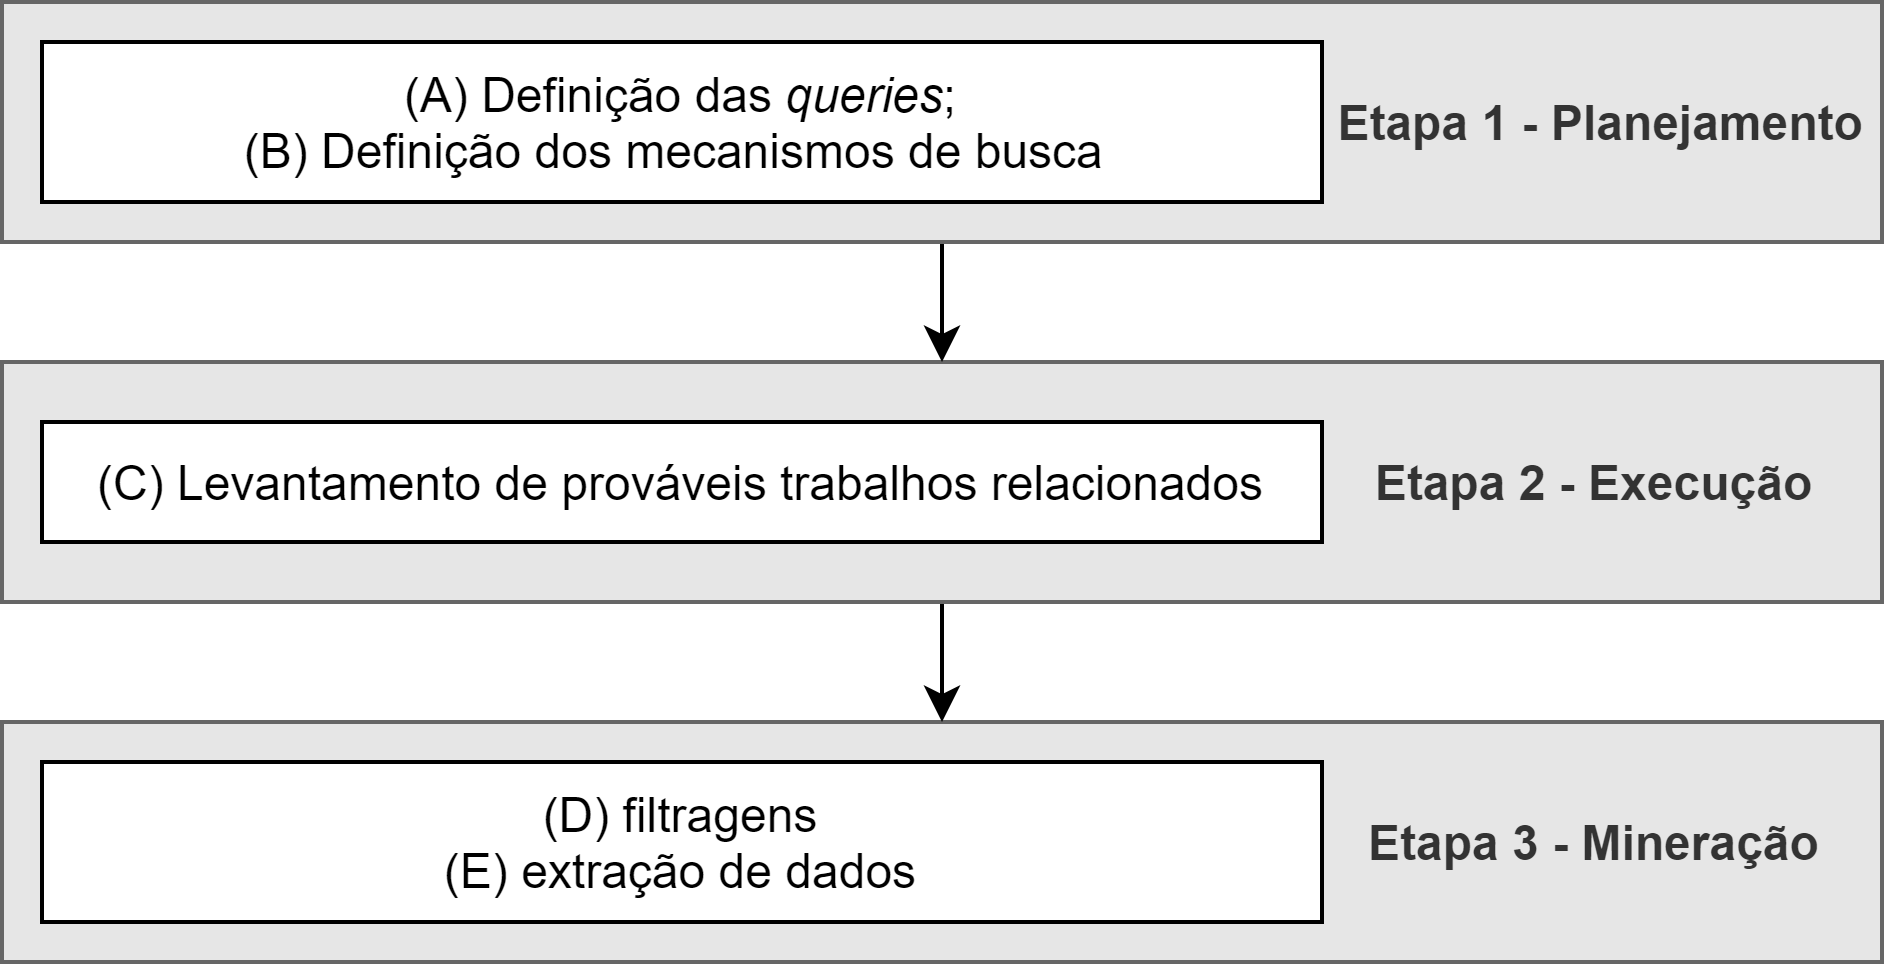
\includegraphics[width=12cm,height=\textwidth,keepaspectratio]{figs/processo_rev_sistematica.png}
\newline \centering{Fonte: Elaborado pelo autor}\label{fig:processo_rev_sistematica}
\end{figure}

Detalham-se as etapas ilustradas na Figura \ref{fig:processo_rev_sistematica} conforme segue:

\begin{enumerate}
    
    \item As \textit{queries} são \textit{strings} que definem a lógica para seleção dos artigos. Para a presente pesquisa procurou-se buscar artigos cujo título ou \textit{keywords} contivessem as palavras ``\textit{Ensemble}'' e ``\textit{learning}'' além de limitar o intervalo de idade da publicação entre o ano de 2015 e o ano de 2020. Faz-se importante destacar que para o ano de 2020 foram considerados os seis primeiros meses.
    
    \item Por conhecida relevância na área da Ciência da Computação e, em especial, na área de Redes de Computadores, duas bases de pesquisa científica foram consideradas para execução das \textit{queries} em seus respectivos motores de busca: IEEExplore\footnote{https://ieeexplore.ieee.org/} e ACM \textit{Digital Library}\footnote{https://dl.acm.org/}.
    
    \item Após execução das \textit{queries} nas bases de pesquisa supracitadas foram obtidos 135 artigos. Uma distribuição da quantidade de artigos obtidos por ano de publicação pode ser observada na Figura \ref{fig:grafico_num_papers}:
    
    
    \begin{figure}[H]
    \centering
    \caption{Distribuição dos artigos obtidos pelo ano de publicação.} 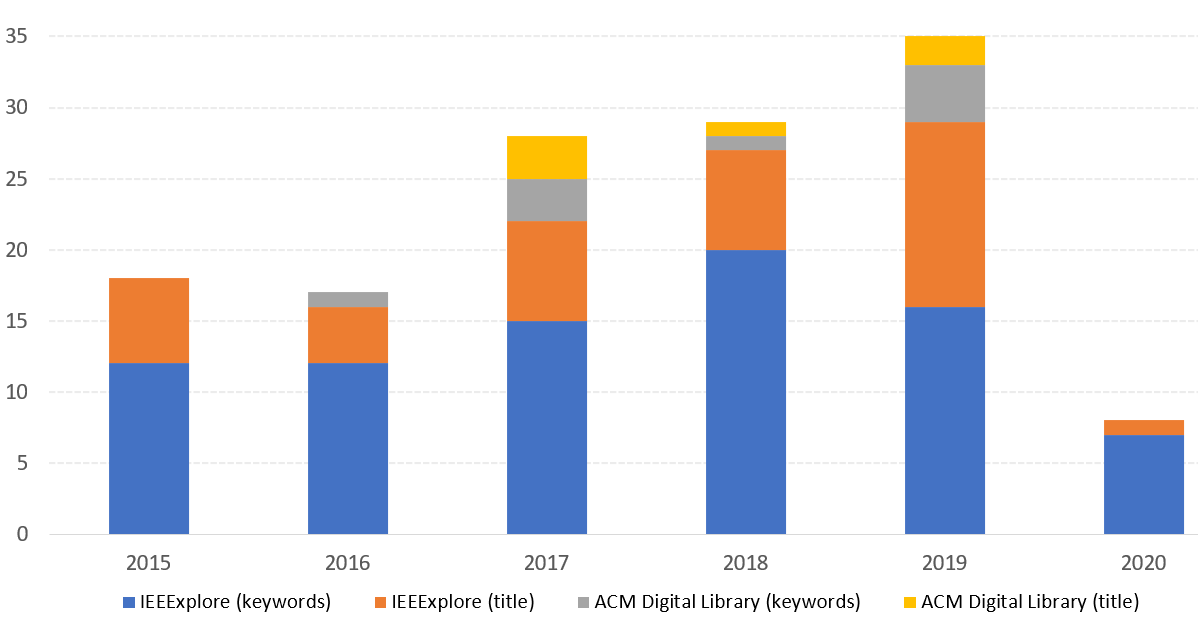
\includegraphics[width=12cm,height=\textwidth,keepaspectratio]{figs/grafico_num_papers.png}
    \newline \centering{ Fonte: Elaborado pelo autor}\label{fig:grafico_num_papers}
    \end{figure}
    
    \item A etapa de filtragem consistiu em eliminar artigos duplicados ou inacessíveis (41 em duplicidade e 2 sem acesso), e, posteriormente, realizou-se a leitura dos 92 artigos restantes onde observou-se que 22 não tinham relação com a linha de pesquisa objetivada nesta Dissertação de Mestrado. Portanto, após a aplicação dos filtros, 68 artigos foram identificados como fortemente relacionados ao tema objeto. A Figura \ref{fig:grafico_processamento_papers} resume a corrente etapa:
    
    
    \begin{figure}[H]
    \centering
    \caption{Detalhamento do resultado após os processos de filtragem dos artigos.} 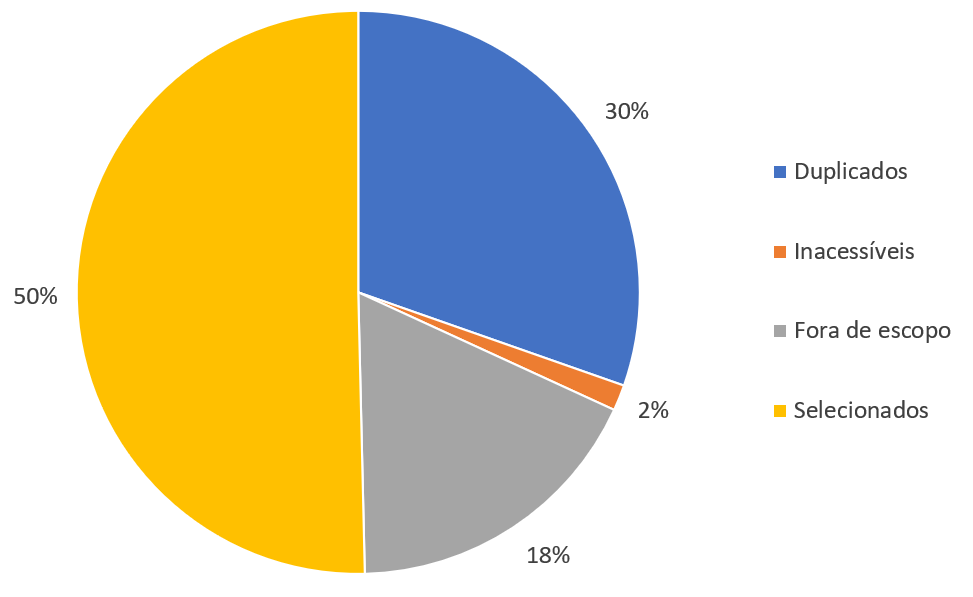
\includegraphics[width=10cm,height=\textwidth,keepaspectratio]{figs/grafico_processamento_papers.png}
    \newline \centering{ Fonte: Elaborado pelo autor}\label{fig:grafico_processamento_papers}
    \end{figure}    
    
    \item Por fim, a quinta etapa consistiu na extração dos dados mais relevantes dos artigos selecionados. Foram extraídos para fins de observação de tendências as seguintes informações:
     \begin{itemize}
         \item Tipo de \textit{Ensemble}: quais as técnicas de agrupamento de classificadores usadas;
         \item \textit{Dataset}: quais as bases de dados usadas para realização dos testes;
         \item Classificadores: quais os classificadores usados para detecção de intrusão;
         \item \textit{Feature selection}: quais algoritmos de seleção de \textit{features} foram usados para redução da dimensionalidade dos \textit{datasets}; 
         \item Resultados: a quais resultados os autores chegaram, como acurácia, \textit{precision}, \textit{recall} e \textit{detection rate}, por exemplo; e
         \item Metodologia: quais materiais foram usados no processo de criação do detector de intrusão (linguagens e softwares).
     \end{itemize}

\end{enumerate}

Para ilustrar todo o processo de Revisão Sistemática da Literatura, desde os detalhes das \textit{queries} até a extração dos dados mais relevantes, a Figura \ref{fig:diagrama_detalhado_rev_sistematica} exibe um fluxograma completo do processo adotado:

\begin{figure}[H]
\centering
\caption{Fluxo detalhado do procedimento realizado na Revisão Sistemática da Literatura. } 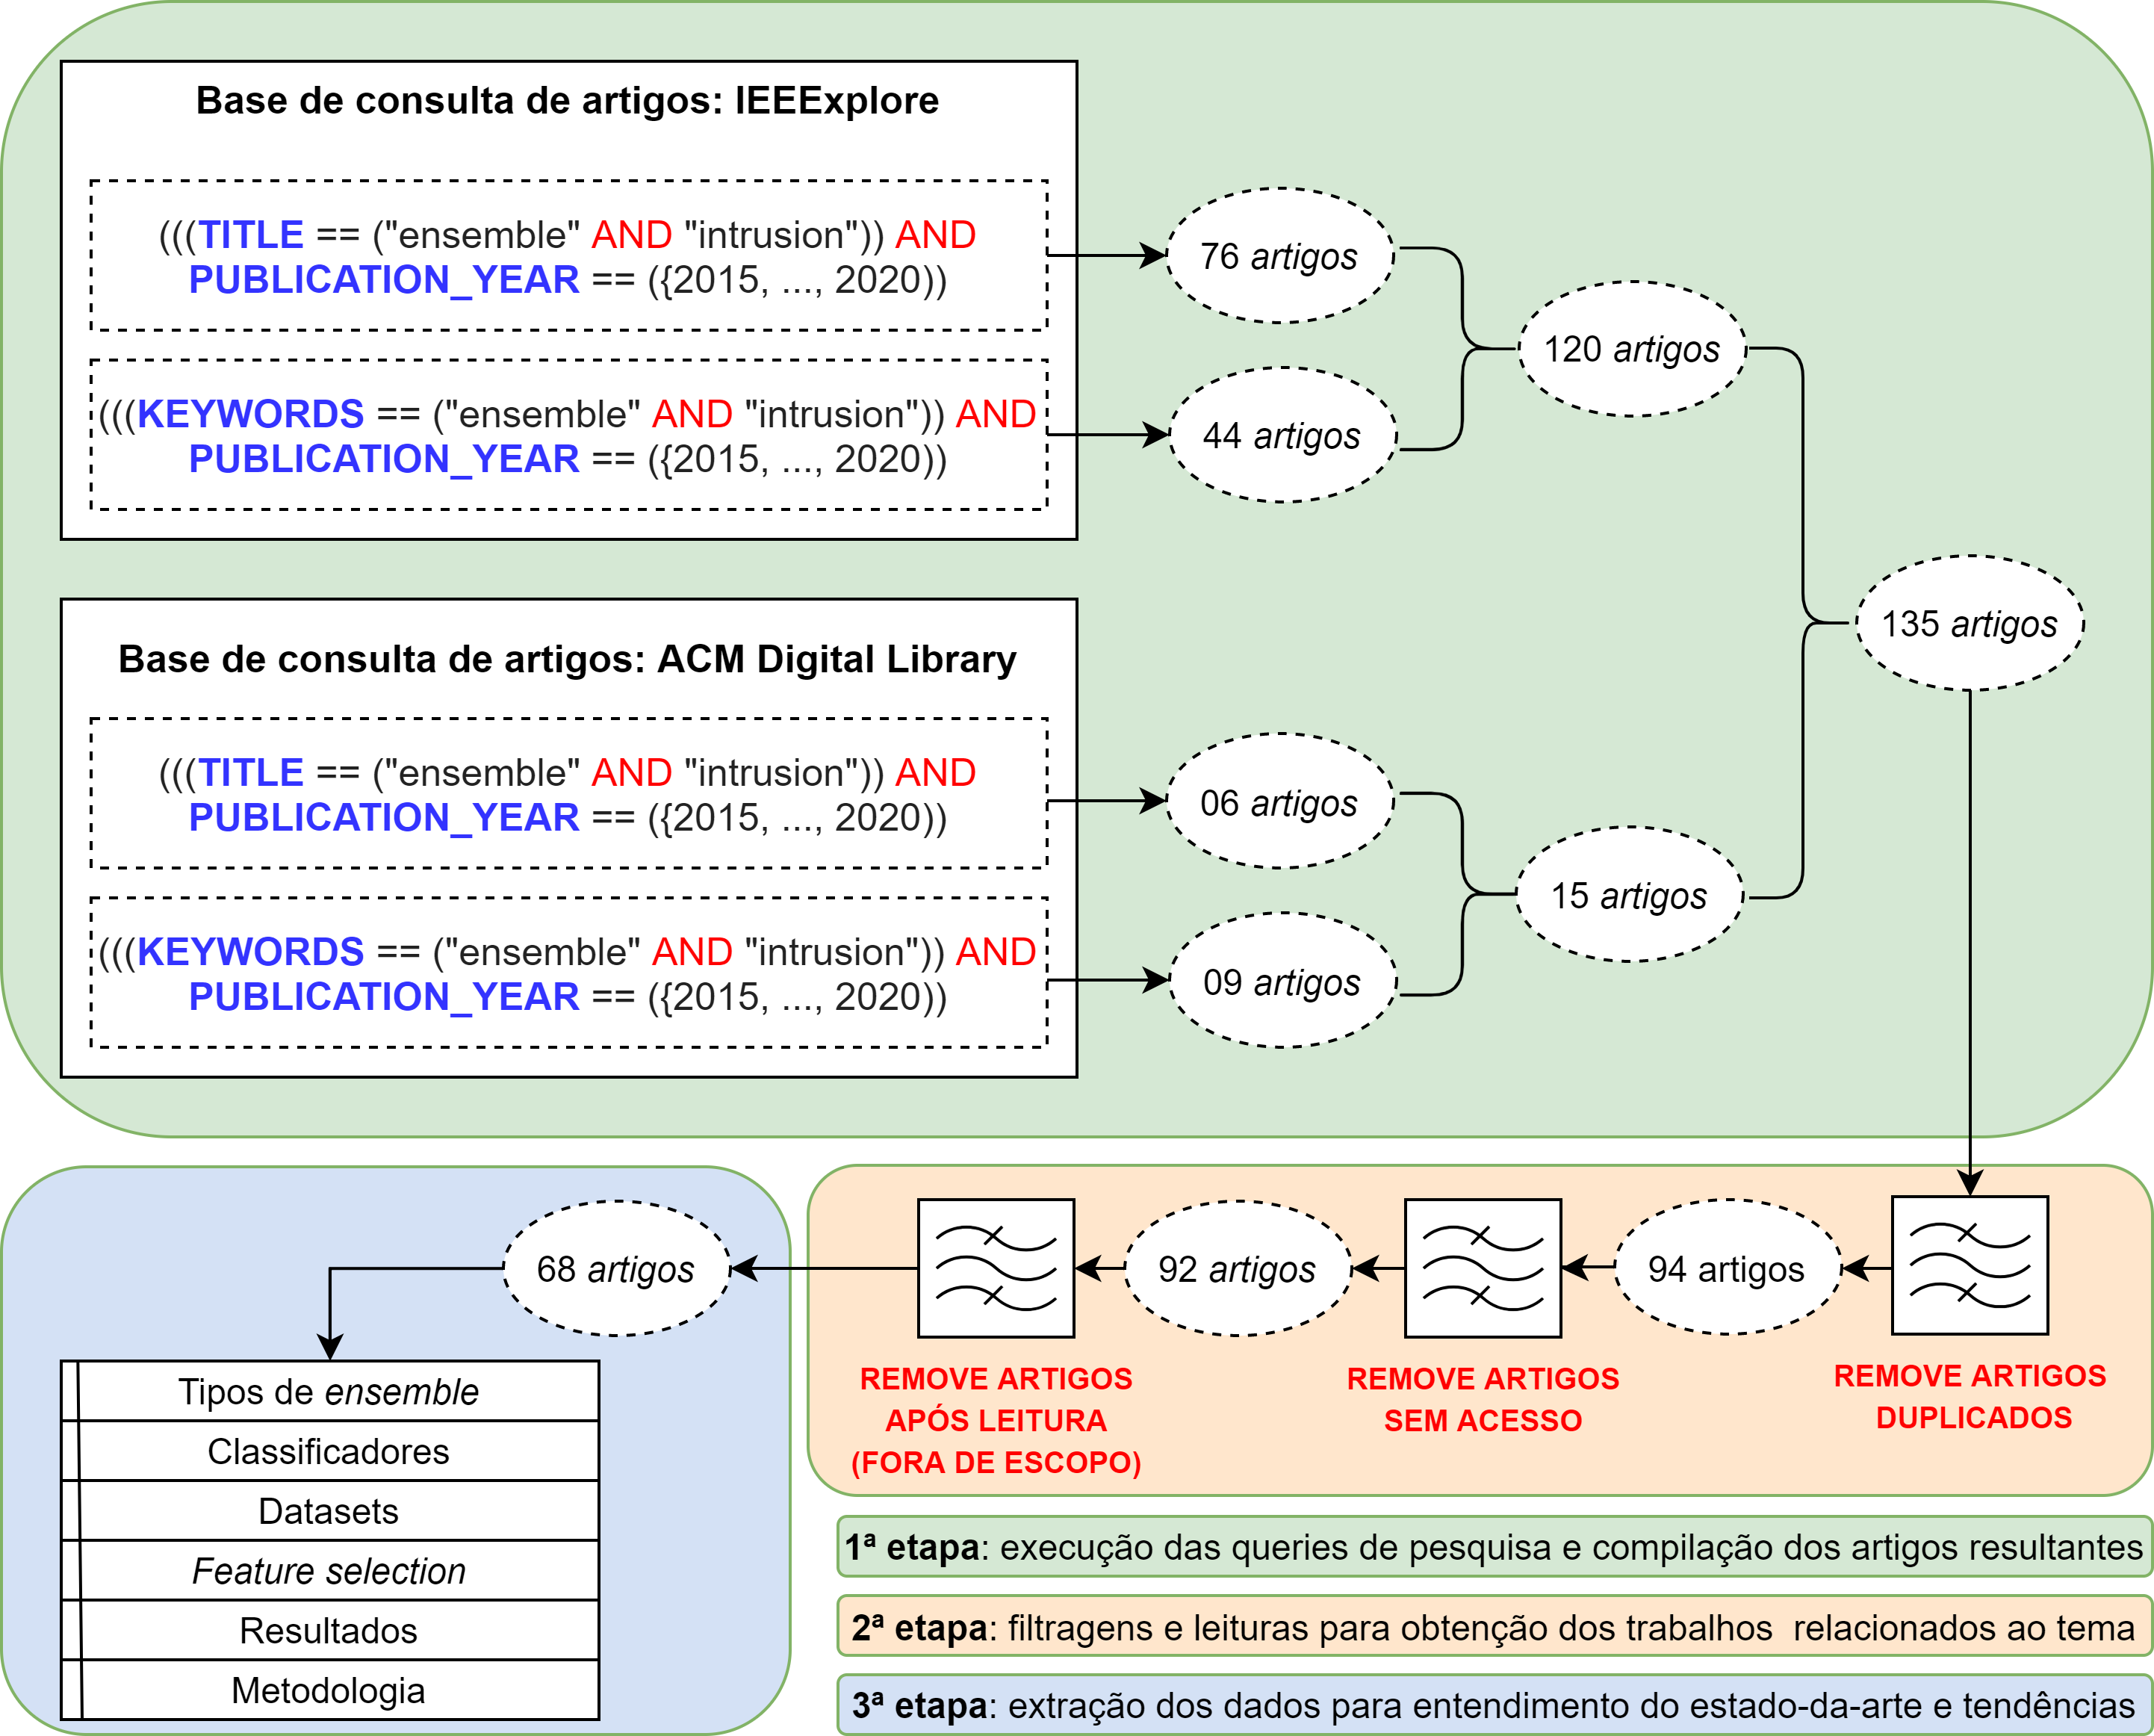
\includegraphics[width=\textwidth,keepaspectratio]{figs/diagrama_detalhado_rev_sistematica.png}
\newline \centering{Fonte: Elaborado pelo autor}\label{fig:diagrama_detalhado_rev_sistematica}
\end{figure}    
    
    
Na sequência os artigos selecionados são resumidos de forma a destacar os elementos mais importantes para relacionamento com a presente pesquisa. Os estudos foram organizados seguindo o seguinte critério:

\begin{itemize}
    \item Detalhamento dos trabalhos correlatos para o ano de 2015 na Subseção \ref{trab_correlatos_15} e compilado de dados extraídos na Tabela \ref{tab:art2015};
    

    \item Detalhamento dos trabalhos correlatos para o ano de 2016 na Subseção \ref{trab_correlatos_16} e compilado de dados extraídos na Tabela \ref{tab:art2016};
    
    \item Detalhamento dos trabalhos correlatos para o ano de 2017 na Subseção \ref{trab_correlatos_17} e compilado de dados extraídos na Tabela \ref{tab:art2017};
    
    \item Detalhamento dos trabalhos correlatos para o ano de 2018 na Subseção \ref{trab_correlatos_18} e compilado de dados extraídos na Tabela \ref{tab:art2018};
    
    \item Detalhamento dos trabalhos correlatos para o ano de 2019 na Subseção \ref{trab_correlatos_19} e compilado de dados extraídos na Tabela \ref{ref:art2019};
    
    \item Detalhamento dos trabalhos correlatos para o ano de 2020 na Subseção \ref{trab_correlatos_20} e compilado de dados extraídos na Tabela \ref{ref:art2020};
    
    
\end{itemize}
    
\subsection{Trabalhos Correlatos - ano de 2015}
\label{trab_correlatos_15}

O trabalho de \citeonline{mehra2015effectual} destaca o quão problemático pode ser o processamento de grande quantidade de dados, o que reforça a necessidade da utilização de técnicas adequadas de \textit{Data Mining} para lidar com tais cenários. Os autores realizaram um experimento utilizando o dataset KDD Cup 1999 que, de início, foi processado pelo algoritmo C4.5\footnote{Algoritmo proposto por \citeonline{quinlan2014c4} para criação de \textit{Decision Trees}.} para geração de \textit{Decisions Trees} (DT - mais detalhes na Subseção \ref{dt}) que, numa segunda etapa, foram agrupadas pelo algoritmo de \textit{Ensemble learning} Adaboost\footnote{Algoritmo de \textit{Ensemble Learning} meta-heurístico proposto por \citeonline{freund1996experiments}.}. Por fim, foi realizada uma integração com o Snort\footnote{Sistema de Detecção de Intrusão de livre distribuição e de código-fonte aberto - https://www.snort.org/.} a fim de se realizar testes efetivos em tempo real. Os autores destacam a obtenção de uma \textit{Detection Rate} de 89.56\% enquanto o valor de \textit{False Alarm Rate} foi de 0.1\% para os testes realizados.

\citeonline{haq2015Ensemble} utilizaram técnicas de \textit{Ensemble learning} tanto para o processo de seleção de \textit{features} quanto para a classificação dos alarmes. Uma lógica de união e intersecção entre as \textit{features} obtidas pelos algoritmos \textit{Best First}\footnote{Função clássica de busca informada trabalha expandindo o nó mais próximo ao objetivo final.}, \textit{Genetic Search}\footnote{Classe de algoritmos genéticos de busca que possuem inspiração nos sistemas biológicos e na natureza.} e \textit{Rank Search}\footnote{Método de busca que leva em consideração um \textit{score} ordenado partindo da classe mais provável.} permitiu uma escolha mais adequada das melhores \textit{features} no dataset NSL-KDD. No processo de classificação o \textit{Ensemble} foi realizado por meio de \textit{Majority Voting}\footnote{Tipo de \textit{Ensemble} por votação onde a classe mais votada é atribuída como rótulo do vetor analisado.} entre os classificadores \textit{Bayesian Network}\footnote{Modelagem gráfica de classificação que é baseada em distribuições de probabilidade multivariadas.}, Naive Bayes\footnote{Modelo de classificador probabilístico que é baseado no teorema Bayesiano.}, \textit{Random Forest}\footnote{Tipo de \textit{Ensemble} que agrupa diversas \textit{Decision Trees} com o objetivo de obter maior desempenho.} e J48\footnote{Uma implementação do algoritmo C4.5 em Java e disponibilizada em forma de código-fonte aberto.}. O modelo proposto obteve uma \textit{True Positive Rate} de 98.0\%  face a uma \textit{False Positive Rate} de 0.021\%. 

Um modelo de \textit{Stacking Ensemble} foi proposto por \citeonline{milliken2015Ensemble}. Os experimentos demonstraram que a análise da entropia entre pares de features de diferentes subsets pode contribuir para a geração de um subset mais adequado para classificação de ataques. Os autores utilizaram o dataset ISCX 2012 como base para os testes juntamente com os classificadores OneR\footnote{Preditor que cria uma regra específica para cada dado baseado em uma tabela de frequências.}, Conjunctive\footnote{Método de classificação que aponta um conjunto de rótulos como resultado e não apenas uma classe.} e Naive Bayes em um modelo de \textit{Stacking} para realização do \textit{Ensemble}. Os experimentos obtiveram como melhor resultado um F-\textit{Score} de 92\%.

\citeonline{amudha2015intrusion} propuseram uma combinação de \textit{Core Vector Machine} (uma derivação do método SVM (\textit{Support Vector Machine}), sobre o qual há mais detalhes na Subseção \ref{svm}) como classificador e \textit{Bagging} como técnica de \textit{Ensemble}. Outros testes foram realizados pelos autores e estão documentados em sua publicação, como a aplicação de Adaboost para \textit{Ensemble} e Naive Bayes, \textit{Decision Tree} e \textit{Random Forest} como classificadores. Entretanto, os melhores resultados no dataset KDD Cup 1999 apontaram para uma acurácia de 98.7\% para detecção de DoS, 98.78\% para ataques de \textit{probe}, 98.16\% para R2L e 98.41\% para U2R utilizando a combinação de \textit{Bagging} e \textit{Core Vector Machine}. Mais detalhes acerca dos tipo de ataque para os \textit{datasets} KDD Cup 1999 e derivados podem ser observados na Seção \ref{secao-datasets}.


Um modelo especialista para detecção de ataques R2L e U2R foi apresentado por \citeonline{sornsuwit2015intrusion}. Trata-se de uma combinação dos classificadores Naive Bayes, \textit{Multilayer Perceptron} (MLP - mais detalhes na Subseção \ref{nn}), \textit{Decision Tree}, \textit{Support Vector Machine} e k-\textit{Nearest Neighbor} (k-NN - mais detalhes na Subseção \ref{knn}) por meio da técnica de \textit{Ensemble} Adaboost. As melhores features no dataset KDD Cup 1999 foram selecionadas por meio da análise de correlação. Os melhores resultados obtidos foram de uma \textit{sensitivity} de 76\% para uma combinação de Naive Bayes e \textit{Multilayer Perceptron} e de uma \textit{specificity} de 99.05\% para uma combinação entre diferentes classificadores Naive Bayes.

\citeonline{gaikwad2015intrusion} apresentaram um modelo que utiliza \textit{bagging} como técnica de \textit{Ensemble} para classificadores REPTree\footnote{Classificador baseado em \textit{Decision Trees} reduzindo a taxa de erro pela observação de ganho e variância.}. Os autores selecionaram as melhores \textit{features} no dataset NSL-KDD usando BIRCH \textit{Hierarquical Clustering}\footnote{Criador de \textit{clusters} não-supervisionado normalmente aplicado a um grande conjunto de dados.}. Os resultados obtidos foram de 99.67\% de acurácia enquanto observou-se uma \textit{False Positive Rate} de apenas 0.3\%. Embora não especifiquem qual classificador fora utilizado como base, \citeonline{sreenath2015intrusion} também modelaram um detector de intrusão usando \textit{bagging} no mesmo NSL-KDD e a acurácia mensurada na detecção foi de 97.85\%. 

Por meio da técnica de \textit{Ensemble one-vs-all}\footnote{Método de classificação que combina diversos classificadores binários independentes.}, \citeonline{ye2015network} combinaram três tipos de classificadores de forma a melhorar a performance na detecção de intrusão para o modelo proposto. Os autores usaram como classificadores algoritmos de \textit{Decision Tree}, \textit{Neural Network} (NN - mais detalhes na Subseção \ref{nn}) e \textit{Support Vector Machines}. O dataset usados nos testes foi o NSL-KDD e não foi especificada qual a técnica de seleção de \textit{features} utilizada. A acurácia obtida na classificação foi de 97.35\%.

\citeonline{robinson2015ranking} apresentaram dois modelos especialistas na detecção de ataques DDoS\footnote{Ataque onde vários hosts maliciosos enviam requisições em larga escala com o objetivo de esgotar a capacidade de processamento do alvo.}. Utilizando \textit{Random Forests} como classificadores os autores modelaram dois \textit{Ensembles}: um com Adaboost e outro com \textit{bagging} a fim de compará-los. O modelo baseado em \textit{bagging} obteve os melhores resultados quando observou-se os valores obtidos de \textit{False Negative Rate}, \textit{False Positive Rate} e \textit{Precision}. A única métrica de avaliação onde o Adaboost se mostrou superior foi a de \textit{Recall}. Todos os testes foram realizados nos datasets LLS-DDoS1.0, CAIDA 2007 e CAIDA Conficker. 

% 18
Por se tratar de um protocolo padrão para acesso remoto em servidores Unix e Linux, no geral, o protocolo SSH é bastante explorado para ataques de dicionário, objetivando o ganho de privilégio remoto para controle de servidores vulneráveis. É o que afirmam \citeonline{alez2015different} em seu experimento, onde os mesmos testaram diferentes métodos de \textit{Ensemble} (\textit{bagging}, \textit{boosting}, \textit{Adaboost}, \textit{MultiboostingAB}\footnote{Classificador que combina diversos \textit{Ensembles} baseados na técnica de \textit{Boosting}.} e \textit{Rotation Forest}\footnote{Uma proposta de \textit{Ensemble} baseado em classificadores \textit{decision forest} que divide o espaço de atributos em diversos \textit{subsets} a serem processados por \textit{bagging}.}) para classificação de alertas oriundos do \textit{honeypot}\footnote{Servidor propositalmente vulnerável útil para geração de estatísticas de ataques.} Euskalert. Os melhores resultados foram com \textit{bagging} onde foi possível mensurar uma \textit{True Positive Rate} de 99.93\%.

% 17
Um \textit{Ensemble} com classificadores C4.5, REPTree e RTree\footnote{Estrutura de dados em árvore que funciona armazenando índices de dados espaciais.} combinados com \textit{bagging} foi apresentado por \citeonline{al2015data}. No pré-processamento os autores escolheram as melhores \textit{features} baseado em correlação para o dataset ISOT e os testes realizados apontaram para uma acurácia de 99.97\%.

Na Tabela \ref{tab:art2015} são organizados os principais detalhes extraídos dos artigos referentes ao ano de 2015:


\begin{longtable}{p{0.4cm}|p{3cm}|p{2cm}|p{3cm}|p{3.5cm}|p{1.5cm}}
\caption{Detalhamento dos artigos obtidos por meio da Revisão Sistemática da Literatura publicados no ano de 2015. Fonte: Elaborado pelo autor.}
\label{tab:art2015}



    
         
\hline
\textbf{ID}\centering & \textbf{Artigo} & \textbf{\textit{Dataset}} & \textbf{Classificadores} & \textbf{\textit{Ensemble}} & \textbf{FS}            \\


\hline
\hline
\endfirsthead \caption[]{Continuação.} \endhead \caption[]{Fim.} \endlastfoot


1 & \citeonline{mehra2015effectual}      & KDD Cup 1999                               & Decision tree                                                     & Boosting              & não especificado                            \\ \hline
2 & \citeonline{haq2015Ensemble}         & NSL-KDD                                    & Bayesian Network,
  Naive Bayes, Random Forest e Decision tree    & Voting                & Best first, Genetic
  search e Rank search  \\ \hline
3 & \citeonline{milliken2015Ensemble}    & ISCX 2012                                  & OneR, Conjunctive e
  Naive Bayes                                 & Stacking              & Entropy pairing of
  features               \\ \hline
4 & \citeonline{amudha2015intrusion}     & KDD Cup 1999                               & Naive Bayes, Decision
  Tree, Random Forest e Core Vector Machine & Boosting e Bagging    & PCA                                         \\ \hline
5 & \citeonline{sornsuwit2015intrusion}  & KDD Cup 1999                               & Naive Bayes,
  Multilayer Perceptron, Decision Tree, SVM e k-NN   & Boosting              & Correlation                           \\ \hline
6 & \citeonline{gaikwad2015intrusion}~   & NSL-KDD                                    & REPTree                                                           & Bagging               & BIRCH hierarchical
  clustering             \\ \hline
7 & \citeonline{sreenath2015intrusion}   & NSL-KDD                                    & Não especificado                                                  & Bagging               & não especificado                            \\ \hline
8 & \citeonline{ye2015network}~          & NSL-KDD                                    & Decision Tree, Neural
  Network e SVM                             & One-to-all            & não especificado                            \\ \hline
9 & \citeonline{robinson2015ranking}     & LLS-DDoS1.0, CAIDA
  2007, CAIDA Conficker & Random Forest                                                     & Boosting e Bagging    & não especificado    \\  
  
\hline

10 & \citeonline{alez2015different}         & Euskalert Honeypot  & não especificado                                                                                                             & Bagging, Boosting,
  MultiboostingAB, Rotation Forest & não especificado                  \\ \hline
        
11 &   \citeonline{al2015data}                & ISTO Botnet         & Decision tree,
  REPtree, Random tree                                                                                        & Bagging                                               & Correlation                 \\ \hline
       




\end{longtable}


\subsection{Trabalhos Correlatos - ano de 2016}
\label{trab_correlatos_16}




% *** 

Um detector de intrusão para redes wireless foi apresentado por \citeonline{alotaibi2016majority}. Utilizando \textit{decision trees} como classificadores os autores modelaram uma técnica de \textit{Ensemble} por \textit{majority voting} onde o rótulo mais votado entre \textit{bagging}, \textit{random forest} e \textit{extraTree}\footnote{Método de classificação que funciona baseado no agrupamento de árvores aleatórias de decisão.} é eleito. Os testes foram realizados no dataset AWID e os resultados apontaram para uma acurácia de 96.32\% e uma \textit{precision}/\textit{recall} de 96\%.


\citeonline{folino2016incremental} destacam dois problemas que normalmente os métodos de \textit{Machine Learning} apresentam quando são utilizados para lidar com situações de classificação de alertas: classes não balanceadas e velocidade dos \textit{streamings} para detecção em tempo-real. Para criar um modelo capaz de enfrentar de forma mais eficaz esses problemas os autores modelaram um \textit{Ensemble} usando \textit{boosting} para combinar os seguintes classificadores: J48, JRIP \textit{rule learner}\footnote{Um modelo de classificação que repetidamente elimina dados que interferem negativamente no modelo de aprendizagem por meio de Árvores de Decisão, reduzindo o erro na atribuição final de classes.}, Naïve Bayes \textit{tree}\footnote{Utiliza \textit{decision trees} como estrutura e atribui rótulos por meio de classificadores Naive Bayes.}, Naïve Bayes, OneR, \textit{logistic model trees}\footnote{Método de classificação que combina \textit{decision trees} com \textit{logistic regression}.}, \textit{logistic regression}\footnote{Método estatístico que permite a previsão de valores, dado um conjunto de observações.}, \textit{decision stumps}\footnote{Modelo de classificação que implementa uma \textit{decision tree} de apenas um nível.} e k-\textit{nearest neighbor}. Os melhores resultados nos testes realizados com o dataset ISCX IDS 2012 obtiveram uma \textit{precision} de  88.28\%, uma \textit{recall} de 80.79\% e uma área sob a  curva \textit{precision}/\textit{recall} de 89\%.

Utilizando uma proposta de \textit{Ensemble} pela implementação de \textit{rotation forests}, \citeonline{tama2016classifier} realizaram um experimento com 20 classificadores a fim de criar um modelo para detecção de intrusão em redes wireless. Diversas combinações foram experimentadas no dataset GPRS e os melhores resultados para detecção nas bases WEP/WPA e WPA2 (que são protocolos para redes wireless) foram obtidos com \textit{best first decision trees} agrupadas pelo algoritmo de \textit{Ensemble} \textit{rotation forest}. A área sob a curva \textit{precision/recall} calculada nos testes foi de 96.01\%.

% 16
\citeonline{mehetrey2016collaborative} apresentaram um detector de intrusão para \textit{cloud computing} que distribui entre os hosts da rede a tarefa de capturar os pacotes e, por amostragem, une num controlador central a rotina de \textit{Ensemble} que fora implementada usando \textit{bagging}. O classificador implementado pelos autores foi o C-Fuzzy \textit{Decision Trees}\footnote{Implementação em C de \textit{decision trees} baseadas em lógica Fuzzy.}. O modelo proposto obteve, em testes com o dataset KDD Cup 1999, uma acurácia de 99.47\%.



%19 
Uma combinação de dois métodos de seleção de \textit{features}, PCA\footnote{\textit{Principal Component Analysis} - processo matemático de transformação de vetores que obtem as possíveis principais \textit{features} por meio da projeção de um conjunto de valores não correlacionados linearmente.} e LDA\footnote{\textit{Linear Discriminant Analysis} - Método que usa estatística, reconhecimento de padrões e \textit{machine learning} para encontrar uma combinação linear de \textit{features} que represente os melhores recursos de um \textit{dataset}.}, aliada ao algoritmo de classificação SVM foi proposta por \citeonline{aburomman2016Ensemble}. Basicamente os pares de \textit{features} em comum obtidos pelos métodos PCA e LDA aplicados ao \textit{dataset} KDD Cup 1999 são processados por um \textit{Ensemble} de \textit{weighted majority voting}\footnote{Método de \textit{Ensemble} que realiza a escolha do melhor rótulo por meio de votação ponderada.} para dez classificadores SVM. Os autores obtiveram uma acurácia de 92.1\% na classificação dos alertas aliados a uma taxa de \textit{false positive} de 1.9\% e uma taxa de \textit{false negative} de 10.8\%.

%22
\citeonline{kiranmai2016extenuate} apresentaram um sistema especialista de detecção de intrusão para \textit{cloud computing} com foco em ataques DDoS. Com um \textit{dataset} próprio. O método de \textit{Ensemble} proposto fora denominado \textit{Consensus Cluster Plus} que uniu classificadores de \textit{clusters} hierárquicos. Os autores não apresentaram resultados que pudessem mensurar a qualidade do sistema apresentado.

%25
Um \textit{Ensemble} usando \textit{Random Committee}\footnote{Conjunto de classificadores que trabalham com os mesmos dados porém com \textit{seeds} diferentes onde o rótulo final é a média das escolhas.} e \textit{voting} foi apresentado por \citeonline{wang2016research}. Unindo classificadores bayesian \textit{network} e \textit{random tree} o método obteve resultados excelentes quando observados pela área sob a curva \textit{precision/recall} no dataset KDD Cup 1999: 99.9\% para Probe e R2L; 100\% para DoS e 99.5\% para U2R.

Na Tabela \ref{tab:art2016} são organizados os principais detalhes extraídos dos artigos referentes ao ano de 2016:


\begin{longtable}{p{0.4cm}|p{3cm}|p{2cm}|p{3cm}|p{3.5cm}|p{1.5cm}}
\caption{Detalhamento dos artigos obtidos por meio da Revisão Sistemática da Literatura publicados no ano de 2016. Fonte: Elaborado pelo autor.}
\label{tab:art2016}



    
         
    \hline

  \textbf{ID} & \textbf{Artigo} & \textbf{\textit{Dataset}} & \textbf{Classificadores} & \textbf{\textit{Ensemble}} & \textbf{FS}            \\


\hline
\hline





12 & \citeonline{alotaibi2016majority} & AWID & Decision Trees, Extra Trees, Random Forests	& Voting entre Bagging, Random forest e Extra tree & não especificado \\ \hline



13 & \citeonline{folino2016incremental}     & ISCX IDS 2012       & Decision tree, Ripper
  rule, NBTree, Naive Bayes, OneR, Logistic model trees, Logistic regression,
  Decision stumps e k-NN & Boosting                                              & não especificado                  \\ \hline
14 & \citeonline{tama2016classifier}~       & GPRS                & 20 algoritmos (melhor
  resultado com Best First Decision Tree)                                                              & Rotation Forest                                       & não especificado                  \\ \hline
15 & \citeonline{mehetrey2016collaborative} & KDD Cup 1999        & Decision tree                                                                                                                & Bagging                                               & não especificado                  \\ \hline
16 & \citeonline{aburomman2016Ensemble}     & KDD Cup 1999        & SVM                                                                                                                          & Weighted Majority
  Voting                            & PCA e LDA                         \\ \hline
17 & \citeonline{kiranmai2016extenuate}     & Próprio             & Hierarchical
  clustering                                                                                                    & Consensus Cluster
  Plus                              & não especificado                  \\ \hline
18 &\citeonline{wang2016research}          & KDD Cup 1999        & Bayesian Network e Random Tree                                                                        & RandomCommittee e Voting                              & não especificado               \\            


\hline

\end{longtable}


\subsection{Trabalhos Correlatos - ano de 2017}
\label{trab_correlatos_17}


%26
\citeonline{miller2017multi} realizaram diversos experimentos no \textit{dataset} NSL-KDD de forma a comparar as seguintes técnicas de \textit{Ensemble}: \textit{majority vote}, \textit{weighted vote}, \textit{naive bayes combination}, \textit{bagging}, \textit{boosting}, \textit{rotation forest} e \textit{random forest}, todos usando classificadores Naive Bayes. Os melhores resultados foram obtidos com \textit{naive bayes combination}, onde foi possível mensurar 84.13\% de alertas corretamente classificados enquanto observou-se 15.86\% de alertas erroneamente classificados.

%27
Um sistema de detecção de intrusão especialista em ataques web foi proposto por \citeonline{kamarudin2017logitboost}. Realizando testes nos \textit{datasets} NSL-KDD e UNSW-NB15 os autores realizaram a seleção de \textit{features} combinando técnicas \textit{wrapper}\footnote{Seleciona as melhores \textit{fetures} em concordância com o classificador. Ou seja, avalia a performance para cada \textit{subset}.} e \textit{filter}\footnote{Independe do classificador, avaliando somente a relação entre as variáveis.}. A técnica de \textit{Ensemble} LogitBoost\footnote{Uma derivação do método Adaboost que aplica a função de custo da Regressão Logística.} incrementou a capacidade de classificadores \textit{random forest} na detecção de ataques. As taxas de detecção observadas foram de 89.75\% e 99.10\% para os \textit{datasets} supracitados, respectivamente.

%28
\citeonline{rajasekaran2017novel} apresentaram um \textit{Ensemble} sequencial para classificação de alertas. Numa primeira camada um classificador EMSVM\footnote{Uma derivação do método de classificação SVM que seleciona um conjunto mais adequado de \textit{features}.} é aplicado e, posteriormente (considerando que apenas dados rotulados como benignos na etapa corrente passam para a próxima etapa) os demais pacotes são classificados pelo k-NN e por SMO\footnote{\textit{Swarm Particle Optimization} - uma área da computação evolutiva que procura, dada uma medida de qualidade, otimizar o problema de forma iterativa buscando a solução mais adequada.}, na ordem apresentada. A seleção das melhores \textit{features} é feita com \textit{Intelligent Agent based Attribute Selection Algorithm} (IAASA)\footnote{Método de seleção de \textit{features} baseado em \textit{information gain ratio} proposto por \citeonline{ganapathy2012intelligent}.}. Os resultados obtidos no \textit{dataset} KDD Cup 1999 foram de uma acurácia aproximada de 97\% para Probe, 97.5\% para DoS, 99\% para U2R e de 86\% para R2L.

%29
\citeonline{chen2017novel} apresentaram um detector de intrusão não-supervisionado que criar um \textit{Ensemble} por meio de \textit{voting} entre quatro algoritmos de \textit{clustering}: DBSCAN\footnote{\textit{Density-based spatial clustering of applications with noise - } agrupa dados próximos no espaço de parâmetros considerando normalmente a distância euclidiana e um número mínimo de pontos.}, \textit{One}-SVM\footnote{Uma derivação do método SVM que aprende apenas os padrões de uma única classe e trabalha de forma a classificar dados futuros de forma binária, ou seja, sendo ou não pertencentes à classe aprendida.}, \textit{Agglomerative Clustering}\footnote{Modelo de \textit{clustering} que os constrói de forma hierárquica. Uma espécie de \textit{Hierarquical Clustering}.} e \textit{Expectation Maximization}\footnote{Abordagem estatística que estima valores para variáveis desconhecidas e otimiza o modelo até que se alcance o resultado ótimo.}. Os resultados obtidos nos experimentos com o \textit{dataset} NSL-KDD foram de uma \textit{detection rate} de 91.03\% e de uma \textit{false positive rate} de 2.26\%.

%31
Após a seleção das melhores \textit{features} no \textit{dataset} NSL-KDD utilizando PSO e seleção baseada em correlação, \citeonline{tama2017improved} implementaram três técnicas de \textit{Ensemble} para classificadores SVM: \textit{majority voting} entre Adaboost e RSM\footnote{\textit{Random Subspace Method} - Técnica de \textit{Ensemble} que busca diminuir a correlação entre preditores treinando \textit{subsets} aleatoriamente.}. O modelo proposto obteve uma acurácia de 85.01\% e uma \textit{false positive rate} de 12.6\%.
 

%32
\citeonline{primartha2017anomaly} criaram \textit{Ensembles} de \textit{majority voting} para classificadores \textit{random forest} a fim de detectar intrusão em três diferentes \textit{datasets}: NSL-KDD, UNSW-NB15 e GPRS. Para os \textit{datasets} supracitados, respectivamente, a acurácia observada foi de 99.57\%, 95.5\% e 91.8\%.

%33
Um sistema de detecção de intrusão baseado em \textit{Ensemble} de \textit{clusters} foi proposto por \citeonline{jabbar2017cluster}. Utilizando o \textit{dataset} Gure KDD e os classificadores ADTree\footnote{Uma implementação de \textit{decision trees} que alterna sistematicamente os nós de decisão e também os rótulos finais buscando incremenetar a performance geral de classificação.}, k-\textit{Means}\footnote{Método de \textit{clustering} que agrupa os dados usando como métrica a proximidade da média do grupo mais próximo.} e k-NN por meio de \textit{weighted majority voting} para classificação binária os testes obtiveram uma acurácia de 99.93\% e uma \textit{detection rate} de 99.8\%. Um experimento similar foi realizado por \citeonline{aravind2017design} onde utilizando diversas métricas de distância os autores obtiveram 90\% de acurácia usando k-\textit{Means} no \textit{dataset} UNSW-NB15. Na mesma linha, \citeonline{ruoti2017intrusion} propuseram um detector que aborda a aplicação de métodos de \textit{Ensemble} por meio de \textit{voting} utilizando diversos classificadores não-supervisionados no \textit{dataset} NSL-KDD, entretanto os autores não divulgaram os resultados obtidos.

%34
\citeonline{belouch2017comparison} realizaram uma comparação entre três técnicas diferentes de \textit{Ensemble}: \textit{booting, bagging} e \textit{Stacking}. Os autores combinaram quatro diferentes classificadores: \textit{decision tree}, Naive Bayes, \textit{nultilayer perceptron} e REP\textit{Tree}. Todos os experimentos foram realizados no \textit{dataset} UNSW-NB15. A publicação documentam todos os resultados sendo possível observar que o melhor \textit{Ensemble} quanto a acurácia foi um \textit{Stacking} de REP\textit{Tree} seguido por um \textit{Stacking} de \textit{decision trees}.


%36
\citeonline{niranjan2017ebjrv} apresentaram um detector de intrusão que combina seleção das melhores \textit{features} usando \textit{information gain ratio} e um esquema de \textit{voting} entre \textit{bagging}, \textit{Random Committee} e \textit{decision tree}. Levando em conta que os dois primeiros utilizam como classificadores \textit{random trees}, os autores performaram testes nos \textit{datasets} NSL-KDD e KDD Cup 1999 onde ambos apontaram para uma \textit{true positive rate} de 100\% e uma \textit{false positive rate} de 0\%.

% AQUI
%37
\citeonline{garg2017enclass} apresentaram um modelo próprio de \textit{Ensemble} usando classificadores \textit{Very Fast Decision Trees}\footnote{Um algoritmo de \textit{machine learning} com foco em \textit{streaming} de dados.} e selecionando as melhores \textit{features} com \textit{Hoeffding bound}\footnote{Modelo matemático que calcula um limite máximo de probabilidade em relação à soma de variáveis aleatórias independentes se desvie de um valor estimado.}. O modelo apresentado obteve uma \textit{detection rate} de 98.58\%. Todos os testes foram realizados no \textit{dataset} KDD Cup 1999.

%38
Três diferentes \textit{datasets} foram utilizados para testar um \textit{Ensemble} de \textit{Support Vector Machines} proposto por \citeonline{reddy2017enhanced}. Usando \textit{Rough set theory} (teoria aplicada à aproximação de conjuntos) para obtenção das melhores \textit{features} os autores obtiveram acurácias de 99.95\%, 100\% e 99.98\% para os \textit{datasets} KDD Cup 1999, HTTP CSIC 2010 e UNB ISCX, respectivamente.

%39
\citeonline{timvcenko2017Ensemble} criaram um modelo de detecção de intrusão que combina diversos métodos de \textit{Ensemble} utilizando como \textit{decision tree} como classificador base. Cada agrupamento utiliza uma técnica: \textit{Bagged tree} (\textit{decision trees} baseadas em \textit{bagging}), Adaboost, Logitboost, Gentleboost (derivação do Adaboost) e RUSboost (algoritmo de \textit{boosting} para balanceamento de classes). As melhores \textit{detection rates} foram obtidas com \textit{bagged tree} e \textit{Gentleboost} obtendo 99.1\% quando testadas no \textit{dataset} UNSB-NB15.

%40

Buscando detectar ataques do tipo Neptune (uma espécie de DoS) no \textit{dataset} NSL-KDD, \citeonline{mkuzangwe2017Ensemble} criaram um classificador binário apto a detectar intrusão diferenciando conexões normais de anormais. Os autores implementaram um \textit{Ensemble} via Adaboost unindo classificadores \textit{decision stump} o que lhes permitiu obter uma acurácia de 87.83\%. O método de seleção de \textit{features} usado no experimento foi o \textit{Information Gain Ratio}.

%43
\citeonline{ludwig2017intrusion} apresentou um detector de intrusão que utiliza uma rede neural para criar um \textit{Ensemble} contendo um \textit{Autoencoder}\footnote{Um tipo de ANN não supervisionada que tem como objetivo reduzir a dimensionalidade de um \textit{dataset}}, uma \textit{Deep Belief Neural Network}\footnote{Uma ANN com muitos neurônios nas camadas intermediárias mas que , por definição, não apresenta ligações entre neurônios de uma mesma camada.}, uma \textit{deep neural network}\footnote{Uma ANN com muitos neurônios nas camadas intermediárias. Não existe consenso sobre a quantidade mínima de neurônios que a definem.}, e uma \textit{Extreme Learning Machine}\footnote{Um modelo de ANN que possui uma ou várias camadas intermediárias e onde não há necessidade de ajustes nos parâmetros dos nós ocultos.}. O autor realizou os experimento no \textit{dataset} NSL-KDD e obteve uma \textit{detection rate} de 97.9\% além de uma acurácia de 92.4\%. O detector apresentado é capaz de realizar classificação binária.

Na Tabela \ref{tab:art2017} estão compilados os detalhes referentes aos artigos publicados no ano de 2017:


\begin{longtable}{p{0.4cm}|p{3cm}|p{2cm}|p{3cm}|p{3.5cm}|p{1.5cm}}
\caption{Detalhamento dos artigos obtidos por meio da Revisão Sistemática da Literatura publicados no ano de 2017. Fonte: Elaborado pelo autor.}
\label{tab:art2017}

    
         
    \hline

  \textbf{ID} & \textbf{Artigo} & \textbf{\textit{Dataset}} & \textbf{Classificadores} & \textbf{\textit{Ensemble}} & \textbf{FS}            \\


\hline
\hline
\endfirsthead \caption[]{Continuação.} \endhead \caption[]{Fim.} \endlastfoot







19 & \citeonline{miller2017multi}         & NSL-KDD                             & Naive Bayes                                                                                                                                                               & Majority vote,
  Weighted sum, ML Naive Bayes, Bagging, boosting, Rotation forest, Random
  forest &   não especificado \\ \hline
20 & \citeonline{kamarudin2017logitboost} & NSL-KDD e UNSW-NB15                 & Random Forests                                                                                                                                                            & Boosting (LogitBoost)                                                                              & Hybrid Feature
  Selection (filter + wrapper)                     \\ \hline
21 & \citeonline{rajasekaran2017novel}   & KDD Cup 1999                        & EMSVM, k-NN, Particle
  Swarm Optimization                                                                                                                                & Sequencial (EMSVM, k-NN e PSO)                                                                     & Intelligent
  Agent based Attribute Selection Algorithm (IAASA)~  \\ \hline
22 & \citeonline{chen2017novel}           & NSL-KDD                             & DBSCAN, One-SVM,
  Agglomerative Clustering e Expectation Maximization                                                                                                    & Voting                                                                                             & não especificado                                                  \\ \hline
23 & \citeonline{tama2017improved}        & NSL-KDD                             & SVM                                                                                                                                                                       & Majority Voting entre
  Boosting e Random Subspace Method                                          & Correlation e PSO                                           \\ \hline
24 & \citeonline{primartha2017anomaly}    & NSL-KDD, UNSW-NB15 e
  GPRS         & Decision Tree                                                                                                                                                             & Voting, Random Forest                                                                              & não especificado                                                  \\ \hline
25 & \citeonline{jabbar2017cluster}       & Gure KDD                            & ADTRee, K-Means e
  k-NN                                                                                                                                                  & Voting                                                                                             & não especificado                                                  \\ \hline


26 & \citeonline{aravind2017design}       & UNSW-NB15                           & k-Means                                                                                                                                                                   & não especificado                                                                                   & não especificado                                                  \\ \hline

27 &\citeonline{ruoti2017intrusion}      & NSL-KDD                             & InterquartileRange,
  K-Means, Xmeans, IsolationForest, Expected Maximization, Mtree, Learning
  Vector Quantization, SelfOrganizingMap e SequentialInformationBottleneck & Voting                                                                                             & não especificado                                                  \\


\hline





28 & \citeonline{belouch2017comparison}   & UNSW-NB15                           & Decision tree, Naive
  bayes, Multilayer perceptron, Reptree                                                                                                              & Boosting, Bagging e
  Stacking                                                                     & não especificado                                                  \\ \hline



29 & \citeonline{niranjan2017ebjrv}       & NSL-KDD e KDD Cup
  1999            & Random tree                                                                                                                                                               & Bagging, Majority
  voting e Random committee                                                      & Information Gain
  Ratio                                          \\ \hline
30 & \citeonline{garg2017enclass}         & KDD Cup 1999                        & Decision tree                                                                                                                                                             & não especificado                                                                                   & Hoeffding bound                                                   \\ \hline
31 & \citeonline{reddy2017enhanced}       & KDD Cup 1999, HTTP
  CSIC, UNB-ISCX & SVM                                                                                                                                                                       & não especificado                                                                                   & Rough Set Theory                                                  \\ \hline
32 & \citeonline{timvcenko2017Ensemble}   & UNSW-NB15                           & Decision tree                                                                                                                                                             & Bagged
  tree, Boosting, LogitBoost, GentleBoost and RUSBoost                                      & não especificado                                                  \\ \hline
33 & \citeonline{mkuzangwe2017Ensemble}   & NSL-KDD                             & Decision stump                                                                                                                                                            & Boosting                                                                                           & Information Gain
  Ratio                                          \\ \hline
34 & \citeonline{ludwig2017intrusion}     & NSL-KDD                             & Autoencoder,
  Deep belief neural network, Deep neural network, e Extreme learning machine                                                                                & não especificado                                                                                   & não especificado                                                  \\ \hline








\end{longtable}

















\subsection{Trabalhos Correlatos - ano de 2018}
\label{trab_correlatos_18}





%46
 Um \textit{Ensemble} de classificadores SVM utilizando \textit{bagging} como técnicas de agrupamento foi proposto por \citeonline{tengl2018collaborative}. O detector de intrusão obteve um \textit{subset} por meio de PCA que fora aplicado no \textit{dataset} NSL-KDD. Os autores dividiram a tarefa de classificação entre três detectores de acordo com três protocolos de redes de computadores presentes no \textit{dataset} supracitado. Um algoritmo genético colabora no processo de escolha dos pesos de forma a potencializar determinado classificador em detrimento de outro no agrupamento. A acurácia obtida nos testes foi de 88.28\%.
 
 %47

O objetivo do detector de intrusão proposto por \citeonline{yuan2018concept} é o processamento de dados em tempo real. Os autores destacam que se observadas propriedades estatísticas de alteração dos dados ao longo de um tempo de monitoramento, em especial a variância entre os ataques, pode ser possível construir um sistema de classificalção mais robusto. Neste sentido os autores propuseram um \textit{Ensemble} baseado em \textit{concept drift incremental learning}. Os classificadores usados foram Naive Bayes, \textit{Stochastic Gradient Descent}\footnote{Técnica iterativa de substituição do gradiente real para uma estimação do mesmo atuando de forma a otimizar uma função objetiva utilizando parâmetros de suavização.} e \textit{Multilayer} Perceptron. Em testes realizados no \textit{dataset} KDD Cup 1999 a acurácia observada foi de 94.91\%.

\citeonline{sun2018double} apresentaram um modelo de detecção de intrusão que combina três técnicas clássicas de \textit{Ensemble}: \textit{bagging, boosting} e \textit{Stacking}. Os classificadores base utilizados foram SVM e k-NN. Com testes realizados no \textit{dataset} NSL-KDD após geração de um \textit{subset} por meio de PCA foi possível mensurar como melhores resultados de acurácia a classificação de pacotes normais com 99.41\% e a de pacotes probe com 93.13\%.

%49
Um modelo de classificação semi-supervisionada foi apresentado por \citeonline{gao2018novel}. Consistindo de duas etapas, num primeiro momento o detector utiliza um \textit{Ensemble} por meio de \textit{weighted voting} composto de \textit{decision trees} e \textit{neural networks} treinado de forma supervisionada, ou seja, com acesso aos rótulos dos dados. Em um segundo momento há a remoção de dados redundantes e ruidosos na amostra do dataset sem rótulos para que o \textit{subset} resultante seja processado pelo mesmo \textit{Ensemble} do primeiro momento. Os autores usaram um \textit{subset} obtido por meio da aplicação de PCA no \textit{dataset} NSL-KDD e a acurácia obtida foi de 84.54\%.

%50
\citeonline{gautam2018Ensemble} propuseram um modelo de detecção de intrusão que agrupa, por meio de \textit{bagging}, três classificadores, sendo eles Naive Bayes, \textit{Adaptative Boost} e PART. O \textit{dataset} usado pelos autores foi o KDD Cup 1999, de onde foram obtidas as melhores \textit{features} observando análises baseadas em entropia e filtragens. Os resultados obtidos apontam para uma acurácia de 99.97\%.

%51
Um sistema de detecção de intrusão para redes wireless foi modelado por \citeonline{vaca2018Ensemble}. Os autores, usando \textit{decision trees} para classificação, testaram quatro técnicas diferentes de \textit{Ensemble}: \textit{bagging, random forests, extra-trees} e XGboost\footnote{Uma implementação baseada em \textit{Extreme Gradient Boosting} (modelo de árvores construído em etapas de forma a otimizar a função de perda e extrair o máximo da capacidade de processamento do hardware) de \textit{decision trees com foco em performance e velovidade. }}. Após o pré-processamento do \textit{dataset} AWID, o \textit{subset} resultante foi melhor processado pela combinação entre \textit{decision trees} e \textit{random forests} que apresentou uma acurácia de 95.87\% na detecção multi-classe.


%52
\citeonline{shen2018Ensemble} apresentaram um detector de intrusão baseado em \textit{Extreme Learning Machine} e optimizado com \textit{bat algorithm} (inspirado no comportamento dos morcegos), que tinha por função eliminar o pior classificador dentre os quatro diferentes \textit{subsets} que foram gerados por meio de seleção \textit{bootstrap} (mais detalhes sobre \textit{bootstrapping} são abordadas em ``\textit{Bagging}'' na Seção \ref{sec:machinelearning}) no \textit{dataset} original. A aplicação do \textit{Ensemble} se deu por \textit{majority voting} entre os três classificadores não eliminados pelo algoritmo de optimização meta-heurístico. Os autores realizaram testes nos \textit{datasets} KDD Cup 1999, NSL-KDD e Kyoto. As acurácias mensuradas foram de 98.94\%, 97.46\% e 99.19\% para os \textit{datasets} supracitados, respectivamente.


%54
Um \textit{Ensemble} por meio de \textit{majority voting} foi proposto por \citeonline{mirza2018computer}. A \textit{label} mais votada por três diferentes classificadores, sendo eles, \textit{logistic regression, neural network} e \textit{decision trees} é atribuída ao dado analisado. O \textit{subset} processado pelo método proposto foi obtido após aplicação do método PCA no \textit{dataset} KDD Cup 1999. A acurácia obtida nos testes foi de 96.14\%.

%56
Uma outra proposta de \textit{Ensemble} por \textit{majority voting} foi apresentada por \citeonline{marir2018distributed}, onde os autores reduzem a dimensionalidade dos \textit{datasets} usando uma \textit{deep believe network} e classificam os dados por meio de um agrupamento de \textit{support vector machines}. Tal modelo fora testado em quatro diferentes \textit{datasets}: NSL-KDD, KDD Cup 1999, UNSW-NB15 e CICIDS 2017, onde as áreas sob as curvas \textit{precision/recall} foram, respectivamente, 98.56\%, 98.44\%, 98\% e 96.30\%.

%60
\citeonline{abdullah2018improving} propuseram um detector de intrusão multi-classe com k-SVM, uma combinação de k-\textit{Means} com \textit{support vector machines}. As melhores \textit{features} no \textit{dataset} NSL-KDD são obtidas após a aplicação de \textit{Genetic Linear Discriminant Analysis} na etapa de pré-processamento. O \textit{Ensemble} fora implementado por meio de \textit{voting}. O modelo apresentou uma \textit{detection rate} de 99.7\%.

%61
Uma comparação entre Adaboost e \textit{bagging} fora realizada por \citeonline{pham2018improving} com o objetivo de construir um sistema de detecção de intrusão mais eficaz. Os autores usaram diferentes classificadores nos testes com o \textit{dataset} NSL-KDD, sendo eles: \textit{decision tree, random forest, decision stump, reptree} e \textit{randomtree}. Para seleção das melhores \textit{features} os autores usaram dois métodos: \textit{information gain ratio} e \textit{leave-one-out}. Os melhores resultados foram obtidos com as \textit{features} selecionadas por meio de \textit{information gain ratio} e classificadas com agrupamento via \textit{bagging} de classificadores \textit{decision tree}, obtendo acurácia de 84.25\%.

%62
\citeonline{zhang2018network} modelaram um detector de intrusão que utiliza uma \textit{sparse autoencoder network} para reduzir a dimensionalidade do \textit{dataset} NSL-KDD. Um \textit{Ensemble} de \textit{neural networks} usando xg\textit{boost} é responsável por classificar os pacotes. Os autores também empregaram a técnica SMOTE para criar pacotes sintéticos buscando aumentar os dados de classes com menos população. As camadas de classificação foram organizadas em forma de árvore binária. Para os ataques DoS, probe, U2R e R2L a F1-\textit{score} observada foi de 98.86\%, 86.02\%, 77.89\% e 98.14\%, respectivamente. Para os pacotes normais foi de 98.98\%.

%63
O trabalho de \citeonline{zwane2018performance} compara diversos classificadores simples com as técnicas de \textit{Ensemble} \textit{bagging}, Adaboost e \textit{random forest}. Usando o \textit{dataset} UNSW-NB15 os autores obtiveram como melhor resultado um \textit{Ensemble} de \textit{random forest} atingindo 98.1\% de área sob a curva ROC. Os demais classificadores usados nos testes foram \textit{multilayer perceptron}, \textit{decision tree}, \textit{bayesian network} e \textit{support vector machine}.

%65
\citeonline{muallem2018tddeht} apresentaram um detector de intrusão que fora testado nos \textit{datasets} Darpa DDoS, Darpa DDoS \textit{Malware} e DoS DNS. O agrupamento de classificadores \textit{hoeffding trees} feito por meio de \textit{Accuracy Updated Ensemble} foi responsável por obter uma acurácia de 100\%.

\citeonline{moustafa2018Ensemble} modelaram um sistema de detecção de intrusão com Adaboost. O foco dos autores foi em criar um modelo específico para ambientes de IoT. A seleção de \textit{features} fora realizada por meio da aplicação do coeficiente de correlação entre os dados dos \textit{datasets} UNSW-NB15 e NIMS. O \textit{Ensemble} criado era composto de três classificadores, sendo eles: \textit{naive bayes}, \textit{decision tree} e \textit{neural network}. O classificador binário obteve uma acurácia de 98.97\% e de 98.29\% para os testes nos \textit{datasets} na ordem em que foram citados.


Na Tabela \ref{tab:art2018} é possível observar os detalhes extraídos dos artigos publicados no ano de 2018:





\begin{longtable}{p{0.4cm}|p{3cm}|p{2cm}|p{3cm}|p{3.5cm}|p{1.5cm}}
\caption{Detalhamento dos artigos obtidos por meio da Revisão Sistemática da Literatura publicados no ano de 2018. Fonte: Elaborado pelo autor.}
\label{tab:art2018}
    
         
    \hline

  \textbf{ID} & \textbf{Artigo} & \textbf{\textit{Dataset}} & \textbf{Classificadores} & \textbf{\textit{Ensemble}} & \textbf{FS}            \\


\hline
\hline
\endfirsthead \caption[]{Continuação.} \endhead \caption[]{Fim.} \endlastfoot


35 & \citeonline{tengl2018collaborative} & NSL-KDD                                         & não
  especificado                                                      & MPML - Multi
  perspetive machine learning       & não
  especificado  \\ \hline
36 & \citeonline{yuan2018concept}        & KDD Cup 1999                                    & Naive bayes,
  Stochastic gradient descent e Multilayer perceptron      & Ensemble based
  Incremental Learning            & não especificado                          \\ \hline
37 & \citeonline{sun2018double}          & KDD Cup 1999                                    & SVM                                                                     & Stacking, Boosting e
  Bagging                   & não especificado                          \\ \hline
38 & \citeonline{gao2018novel}           & NSL-KDD                                         & Decision trees e
  Neural network                                       & Voting                                           & PCA                                       \\ \hline
39 & \citeonline{gautam2018Ensemble}     & KDD Cup 1999                                    & Naive bayes, Boosting
  e PART                                          & Bagging                                          & Information Gain
  Ratio                  \\ \hline
40 & \citeonline{vaca2018Ensemble}       & AWID                                            & Decision trees                                                          & Bagging, Random
  forests, Extra trees e XGBoost & Correlation                         \\ \hline
41 & \citeonline{shen2018Ensemble}       & KDD Cup 1999, NSL-KDD
  e Kyoto                 & Neural network                                                          & Bagging, Majority
  voting                       & não especificado                          \\ \hline

\hline






42 & \citeonline{mirza2018computer}      & KDD Cup 1999                                    & Neural network,
  Decision tree e Logistic regression                   & Voting                                           & PCA                                       \\ \hline
43 & \citeonline{marir2018distributed}   & NSL-KDD, KDD Cup
  1999, UNSW-NB15 e CICIDS2017 & SVM                                                                     & Voting                                           & DBN - Deep believe
  network              \\ \hline
44 & \citeonline{abdullah2018improving}  & NSL-KDD                                         & k-Means e SVM                                                           & Voting                                           & Genetic Linear
  Discriminant Analysis    \\ \hline
45 & \citeonline{pham2018improving}      & NSL-KDD                                         & Decision forest,
  Random forest, Decision stump, REPtree e Random tree & Bagging e Boosting                               & Information Gain
  Ratio e Leave-one-out  \\ \hline
46 & \citeonline{zhang2018network}       & NSL-KDD                                         & Neural network                                                          & Boosting                                         & não especificado                          \\ \hline
47 & \citeonline{zwane2018performance}   & UNSW-NB15                                       & Decision stump,
  REPtree                                               & Bagging, Boosting e
  random forests             & não especificado                          \\ \hline
48 & \citeonline{muallem2018tddeht}      & DARPA DDoS, DARPA
  DDoS Malware, DoS DNS       & Hoeffding trees                                                         & Accuracy Updated
  Ensemble                      & Information Gain
  Ratio    

\\ \hline

49 & \citeonline{moustafa2018Ensemble}~       & UNSW-NB15 e NIMS                                 & Naive bayes, Decision
  tree e Neural network                                            & Boosting                                               & Correlation
  coefficient                                          \\ \hline








\end{longtable}





\subsection{Trabalhos Correlatos - ano de 2019}
\label{trab_correlatos_19}


Um sistema de detecção de intrusão em cascata foi proposto por \citeonline{labonne2019cascade}. Trata-se de uma sequência de \textit{neural networks} especialistas em detectar um tipo de ataque nos \textit{datasets} NSL-KDD e KDD Cup 1999. De forma sequencial, o \textit{subset} resultante de cada detecção é então processado pelo detector especialista posterior, de forma com que, no final do processamento em cascata, seja possível a detecção de cada uma das classes presentes nos \textit{datasets}. As acurácias mensuradas foram de 95.27\% para o \textit{dataset} KDD Cup 1999 e de 97.77\% para o NSL-KDD.

\citeonline{liang2019clustering} propuseram um detector de intrusão que integra um classificador não supervisionado usando k-\textit{Means} com um classificador supervisionado usando \textit{support vector machines}. O \textit{Ensemble} proposto é dado de forma sequencial, onde o modelo inicialmente agrupa os dados com k-\textit{Means} e depois os classifica usando \textit{support vector machines}. Em testes realizados com o \textit{dataset} NSL-KDD foi possível observar uma acurácia de 99.45\% e uma \textit{detection rate} de 99.04\%.

%69
O classificador apresentado por \citeonline{gao2019research} possui a capacidade de balancear o tamanho das amostras de treinamento buscando construir um modelo adaptativo de detecção de intrusão. Os autores implementaram um \textit{Ensemble} por meio de \textit{weighted voting} entre  classificadores \textit{decision tree}, \textit{random forest}, k-NN, \textit{logistic regression}, \textit{support vector machines} e \textit{deep neural network}. Foi usado PCA para redução da dimensionalidade do \textit{dataset} NSL-KDD. A acurácia observada nos testes foi de 84.23\%.


%71
Um \textit{Ensemble} para seleção das melhores \textit{features} no \textit{dataset} Kyoto foi proposto por \citeonline{salo2019clustering}. As \textit{features} em comum (\textit{and}) dentre os métodos \textit{information gain}, \textit{correlation} e \textit{significance} foram usadas na geração de um \textit{subset} que foi processado pelos classificadores k-\textit{Means}, \textit{support vector machine}, k-NN, \textit{random forests} e \textit{quadratic discriminant analysis}. Os melhores resultados foram obtidos com k-NN onde fora observada uma acurácia de 82.28\%.

%72
\citeonline{montalbo2019comparative} apresentaram uma comparação entre diversos métodos de \textit{Ensemble}, sendo eles: Adaboost, \textit{gradient boost}, \textit{random forest} e \textit{extra tree}. Com testes realizados em um \textit{subset} gerado pela seleção das melhores \textit{features} observando o desvio padrão entre os dados do \textit{dataset} NSL-KDD os autores obtiveram para os quatro métodos de \textit{Ensemble} os mesmos resultados de acurácia, \textit{precision} e \textit{recall}, sendo todos eles 99.9\%.

%74
Um sistema de detecção de intrusão focado em ataques DDoS foi modelado por \citeonline{das2019ddos}. Os autores criaram um \textit{Ensemble} por meio de \textit{majority voting} entre os classificadores \textit{multilayer perceptron}, \textit{support vector machine}, k-NN, e \textit{decision tree}. Usando o \textit{dataset} NSL-KDD nos testes foi possível obter uma acurácia de 99.77\% junto a uma \textit{false positive rate} de 0.23\%.

%77
\citeonline{he2019Ensemble} propuseram um modelo de \textit{Ensemble} para seleção de \textit{features}. De acordo com os autores o modelo consiste em aplicar um número ímpar de algorítmos de \textit{feature selection} e, por meio de votação simples, gerar um \textit{subset} contendo as escolhas do modelo. Três \textit{datasets} foram usados nos experimentos: KDD Cup 1999, CICIDS 2017 e UNSW-NB15. Quatro diferentes classificadores foram empregados a fim de se observar a melhoria nos resultados antes e depois do aplicação do \textit{Ensemble}: \textit{decision tree}, k-NN, \textit{multilayer perceptron} e \textit{support vector machine}. O melhor resultado obtido apontou para uma acurácia de 99.4\%. Uma outra abordagem no mesmo sentido foi feita por \citeonline{binbusayyis2019identifying} onde o \textit{Ensemble} selecionou as melhores \textit{features} usando ReliefF\footnote{Método se seleção de \textit{features} baseado em filtragem particularmente sensível a interação entre as variáveis.}, \textit{information gain ratio}, \textit{consistency} e \textit{correlation}. Os autores usaram \textit{random forests} para classificação. Em testes com os \textit{datasets} KDD Cup 1999, NSL-KDD, UNSW-NB15, e CICIDS 2017 os resultados de acurácia foram 99.97\%, 99.89\%, 95.87\% e 99.88\%, respectivamente.



%78 
O sistema de detecção de intrusão apresentado por \citeonline{lu2019error} consiste em separar por camadas os pacotes a serem classificados de acordo com os protocolos TCP\footnote{Protocolo da camada de transporte do Modelo de Referência OSI que provê comunicação confiável.}, UDP\footnote{Protocolo da camada de transporte do Modelo de Referência OSI que não tem como foco a confibilidade mas sim o desempenho.} e ICMP\footnote{Protocolo da camada de rede do Modelo de Referência OSI útil para monitoramento e extração de estatísticas qualitativas.}. Para cada grupo de pacotes são aplicados classificadores binários dispostos em cascata de forma com que, no final do processo, seja possível realizar uma classificação multiclasse completa. Os autores realizaram testes com o \textit{dataset} NSL-KDD usando os classificadores \textit{support vector machine, decision tree,} Bayes \textit{network}, REPTree, k-NN, BFTree\footnote{\textit{Decision trees} inspiradas no método de busca \textit{Best First}.}, SimpleCart\footnote{Biblioteca que provê classificação e regressão baseado em \textit{Decision trees}.} e Naive Bayes. Os resultados foram superiores aos comparados \textit{bagging}, \textit{boosting} e \textit{Stacking}, atingindo uma acurácia de 95.33\% para detectar ataques DoS, 91.14\% para ataques probe, 55.21\% para R2L e 1.42 para U2R, além de uma acurácia de 98.02\% na detecção de pacotes benignos.

%84
\citeonline{illy2019securing} motivaram-se em criar um sistema de detecção de intrusão para IoT que apresentasse o menor número possivel de \textit{false positive rate}. Usando diversas possibilidade de combinações entre classificadores k-NN e \textit{decision tree} além dos métodos de \textit{Ensemble} \textit{bagging, boosting, random forest} e \textit{voting} os autores apresentaram diversos cenários de configuração e seus respectivos resultados em testes com o \textit{dataset} NSL-KDD. Os melhores valores de acurácia para classificação binária foram de 85.81\% (\textit{decision tree} + \textit{bagging}) e para multiclasse de 83.83\% (\textit{voting} entre k-NN, \textit{random forest, bagging} e \textit{boosting} de \textit{decision trees}). 





Em experimentos com os \textit{datasets} NSL-KDD e UNSW-NB15, \citeonline{hsu2019toward} e \citeonline{tama2019tse} apresentaram modelos de detecção de intrusão usando \textit{Ensembles} seja na classificação ou na seleção de \textit{features}. O primeiro agrupou usando \textit{Stacking} no processo de detecção os classificadores \textit{support vector machine, autoencoder} e \textit{random forest}. Já o segundo, usou um \textit{Ensemble} de \textit{majority voting} para \textit{rotation forest} e \textit{bagging} no processo de classificação, além de aplicar um seletor de \textit{features} que faz um \textit{Ensemble} de \textit{particle swarm optimization}, \textit{ant colony} e \textit{genetic algorithm}. Os resultados de acurácia dos primeiros autores indicam 91.7\% com NSL-KDD e 91.8\% com UNSW-NB15, enquanto os demais autores obtiveram 85.79\% e 91.27\% na mesma sequência.


Na Tabela \ref{ref:art2019} estão organizados os principais detalhes extraídos dos artigos publicados no ano de 2019:




\begin{longtable}{p{0.4cm}|p{3cm}|p{2cm}|p{3cm}|p{3.5cm}|p{1.5cm}}
\caption{Detalhamento dos artigos obtidos por meio da Revisão Sistemática da Literatura publicados no ano de 2019. Fonte: Elaborado pelo autor.}
\label{ref:art2019}
         
    \hline

  \textbf{ID} & \textbf{Artigo} & \textbf{\textit{Dataset}} & \textbf{Classificadores} & \textbf{\textit{Ensemble}} & \textbf{FS}            \\


\hline
\hline
\endfirsthead \caption[]{Continuação.} \endhead \caption[]{Fim.} \endlastfoot


50 & \citeonline{labonne2019cascade}          & KDD Cup 1999 e
  NSL-KDD                         & Neural network                                                                           & Voting                                                 & não
  especificado                                                 \\ \hline
51 & \citeonline{liang2019clustering}~        & NSL-KDD                                          & K-means e SVM                                                                            & Sequencial (k-Means e
  SVM)                           & não especificado                                                   \\ \hline
52 & \citeonline{gao2019research}             & NSL-KDD                                          & Decision tree, Random
  forest, k-NN, Logistic regression, SVM e Deep neural network     & Voting                                                 & PCA                                                                \\ \hline
53 & \citeonline{salo2019clustering}          & Kyoto                                            & k-Means, SVM, k-NN,
  Random forest e QDA                                                & Usado na seleção de
  features                         & Information Gain,
  Correlation e Significance                     \\ \hline
54 & \citeonline{montalbo2019comparative}     & NSL-KDD                                          & Não especificado                                                                         & Boosting, Gradient
  boost, Random forest e Extra tree & High relevance
  (desvio padrão)                                   \\ \hline
55 & \citeonline{das2019ddos}                 & NSL-KDD                                          & Multilayer
  perceptron, SVM, k-NN e Decision tree                                       & Voting                                                 & não especificado                                                   \\ \hline








56 & \citeonline{he2019Ensemble}              & kDD Cup 1999,
  CIDDS-001 e UNSW-NB15            & Decision tree, k-NN,
  Multilayer perceptron e SVM                                       & Voting                                                 & Ensemble feature
  selection entre MDI, RFC e Stability Selection  \\ \hline


57 & \citeonline{binbusayyis2019identifying}~ & KDD Cup 1999,
  NSL-KDD, UNSW-NB15, e CICIDS2017 & Decision tree                                                                            & Random forest                                          & Ensemble entre
  ReliefF, InfoGain, Consistency e Correlation      \\ \hline



58 & \citeonline{lu2019error}                 & NSL-KDD                                          & SVM, Decision tree,
  Bayesian network, REPTree, k-NN, BFTree, SimpleCart e Naive Bayes~ & Bagging, Boosting,
  Stacking e ML-SCEN                & não especificado                                                   \\ \hline
59 & \citeonline{illy2019securing}            & NSL-KDD                                          & Decision tree, k-NN e
  Random forest                                                    & Bagging, Voting e
  Boosting                           & não especificado                                                   \\ \hline
60 & \citeonline{hsu2019toward}               & NSL-KDD e UNSW-NB15                              & Autoencoder, SVM e
  Random forest                                                       & Stacking                                               & não especificado                                                   \\ \hline
61 & \citeonline{tama2019tse}                 & NSL-KDD e UNSW-NB15                              & não especificado                                                                         & Voting entre Rotation
  forest e Bagging               & Ensemble entre PSO,
  Ant colony e Genetic algorithm    \\ \hline





\end{longtable}


\subsection{Trabalhos Correlatos - ano de 2020}
\label{trab_correlatos_20}

A presente subseção elenca os trabalhos relacionados obtidos por meio de Revisão Sistemática da Literatura para o ano de 2020. Destaca-se que por se tratar do ano em que os experimentos foram finalizados e dissertação avaliada por meio de qualificação e defesa, os trabalhos aqui documentados levaram em consideração os seis primeiros meses do ano de 2020 como datas de publicação.

\citeonline{kyatham2020novel} apresentaram um modelo autoral de \textit{Ensemble} para dois classificadores baseado em probabilidade. Utilizando MLP e k-NN os autores realizaram experimentos nos \textit{datasets} NSL-KDD e CICIDS-2017. Os resultados apontaram, em detecção multiclasse para os \textit{datasets} supracitados respectivamente, para uma acurácia de 97.05\% e 99.68\%, uma \textit{precision} 98\% e 100\%, uma \textit{recall} de 97\% e 100\% e um F1-Score de 97\% e 100\%.

Uma série de testes com diversos algoritmos de \textit{Ensemble} foi realizada por \citeonline{lower2020study} no \textit{dataset} NSL-KDD. Os autores implementaram \textit{Voting} (entre k-NN, \textit{Decision Tree}, MLP e \textit{Logistic Regression}) \textit{Bagging}, \textit{Random Forest} e Adaboost (todos usando \textit{Decision Trees} como classificadores). Os resultados médios de acurácia, \textit{precision} e F1-Score foram de 81.2\%, 72.5\% e 82\% para \textit{Voting}; 85.4\%, 77.1\% e 84.7\% para \textit{Bagging} e os melhores valores de acurácia, \textit{precision} e F1-Score para os métodos \textit{Random Forest} e \textit{Adaboost} foram de 86.3\%, 78.6\% e 85.7\% para o primeiro e de 86.5\%, 78.5\% e 85.8\% para o último.


\citeonline{olasehinde2020evaluation} realizaram experimentos no \textit{dataset} UNSW-NB15 a fim de se obter qual a melhor hipótese de meta-classificador (classificador da segunda camada) para um modelo de detecção de intrusão usando \textit{Stacking}. Realizando as classificações da primeira camada com k-NN, Naive Bayes e \textit{Decision Tree} os autores testaram algumas possibilidades de meta-classificadores e compararam os resultados. Utilizando três \textit{subsets} diferentes, os melhores resultados foram utilizando \textit{Decision Trees} na segunda camada apontando para uma acurácia média de 98.56\%.


Aplicando \textit{Deep Learning} para detecção de intrusão, \citeonline{alkadi2020deep} implementaram uma \textit{Bidirectional Long Short-Term Memory Neural Network} no \textit{dataset} UNSW-NB15 (embora também tenham realizado experimentos em outro \textit{dataset} que extrapola o escopo da presente dissertação). Um método autoral de \textit{Ensemble} denominado \textit{Deep Blockchain Framework} foi implementado também. A melhor acurácia obtida nos testes foi de 99.41\% com 60 nós na camada intermediária.

\citeonline{folino2020p2p} apresentaram um framework para escolha de métodos de \textit{Ensemble} baseado na acurácia visando diminuir as \textit{false positive rate} e \textit{false alarm rate}. Uma complexa combinação dos classificadores \textit{Decision Tree}, \textit{JRIP Rule Learner}, Naive Bayes \textit{Tree}, Naive Bayes, One-R, \textit{Logistic Model Trees}, \textit{Logistic Regression}, \textit{Decision Stumps} e k-NN foi apresentada de forma a modelar \textit{Ensembles} dinamicamente, ou seja, escolhendo a melhor combinação dentre os classificadores supracitados. Os testes foram realizados no \textit{dataset} CICIDS-2017 e os resultados apresentados pelos autores documentam um decremento de custo computacional no processamento dos dados. Os autores não informaram resultados para a detecção de intrusão. 

Um sistema de detecção de intrusão especialista em detectar ataques web foi apresentado por \citeonline{tama2020enhanced}. Um \textit{Ensemble} por meio de \textit{Stacking} foi implementado, entretanto, ao invés de usar classificadores convencionais, os autores usaram outros métodos de \textit{Ensemble} como \textit{Random Forest}, \textit{Gradient Boost Machine} e XG\textit{boost} para criar os \textit{Stackings}. Quatro diferentes \textit{datasets} foram testados: CICIDS-2017, HTTP-CSIC-2010, NSL-KDD e UNSW-NB15. O resultado médio de acurácia informado pelos autores foi de 96.07\% para o modelo proposto, sendo o melhor resultado obtido no CICIDS-2017 com 99.98\%.

Uma combinação de XG\textit{boost} com \textit{Particle Swarm Optimization} foi proposto por \citeonline{jiang2020network}. Os autores implementaram um sistema de detcção de intrusão multiclasse que fora testado no \textit{dataset} NSL-KDD. O trabalho compara os resultados com outros diversos métodos de \textit{Ensemble}. A média da \textit{precision} (AP - \textit{averaged precision}) obtida nos testes foi de 90\%, 79\%, 94\%, 15\% e 49\% para detectar pacotes benígnos, probe, DoS, U2R e R2L, respectivamente.





\begin{longtable}{p{0.4cm}|p{3cm}|p{2cm}|p{3cm}|p{2.0cm}|p{3cm}}
\caption{Detalhamento dos artigos obtidos por meio da Revisão Sistemática da Literatura publicados no ano de 2020. Fonte: Elaborado pelo autor.}
\label{ref:art2020}
         
\hline

\textbf{ID} & \textbf{Artigo} & \textbf{\textit{Dataset}} & \textbf{Classificadores} & \textbf{\textit{Ensemble}} & \textbf{FS}            \\


\hline
\hline
\endfirsthead \caption[]{Continuação.} \endhead \caption[]{Fim.} \endlastfoot


62 &
\citeonline{kyatham2020novel} & 
CICIDS-2017 e NSL-KDD & 
k-NN e \textit{Multilayer perceptron} & 
Próprio &
não especificado                                \\ \hline

63 &
\citeonline{lower2020study} & 
NSL-KDD & 
\textit{Decision tree}, k-NN, \textit{Multilayer perceptron} e \textit{Logistic regression}
 & 
Voting, Bagging e Boosting &
não especificado                                \\ \hline

64 &
\citeonline{olasehinde2020evaluation} & 
UNSW-NB15 & 
k-NN, Naive Bayes e \textit{Decision Tree} & 
Stacking &
\textit{Consistency}, \textit{Information} e \textit{Correlation}                                \\ \hline

65 &
\citeonline{alkadi2020deep} & 
UNSW-NB15 & 
Neural network & 
não especificado &
não especificado                                \\ \hline

66 &
\citeonline{folino2020p2p} & 
CICIDS-2017 & 
\textit{Decision tree}, Jrip \textit{rule learn}, Naive bayes, \textit{Logistic regression}, \textit{Decision stumps} e k-NN & 
Voting &
\textit{bag-of-pattern}                                \\ \hline

67 &
\citeonline{tama2020enhanced} & 
NSL-KDD, UNSW-NB15, HTTP-CSIC-2010 e CICIDS-2017 & 
não especificado & 
Stacking &
não especificado                                \\ \hline

68 &
\citeonline{jiang2020network} & 
NSL-KDD & 
PSO & 
Boosting &
não especificado                                \\ \hline



\end{longtable}

\subsection{Compilação dos Resultados para os Trabalhos Obtidos}
\label{compilacao-rsl}

A presente Seção documenta o processo de compilação dos trabalhos obtidos por meio da Revisão Sistemática da Literatura de forma a destacar as tendências e os resultados. Destaca-se que os números referentes ao ano de 2020 foram duplicados para que fosse possível obter uma normalização pela quantidade de meses dos demais anos. Como os artigos publicados em 2020 foram obtidos pelos seis primeiros meses do ano, duplicando os números foi possível simular uma tendência para o ano em questão. Reitera-se portanto que os números referentes ao ano de 2020 não são reais mas sim uma projeção. Os números reais são o resultado da metade dos valores projetados.  

\subsubsection{Tendências extraídas - visualização das características}
\label{sub-tendencias}


Uma análise quantitativa de três variáveis (\textit{dataset}, classificador e \textit{Ensemble}) permitiu a visualização das tendências para características fundamentais dos trabalhos obtidos. Tal análise de faz importante para servir de base na escolha das técnicas a serem empregadas na metodologia da presente pesquisa. A Figura \ref{fig:tend_dataset} traz uma análise dos \textit{datasets} mais utilizados:

\begin{figure}[H]
\centering
\caption{\textit{Datasets} utilizados - visualização ano a ano.}
\includegraphics[width=\textwidth,keepaspectratio]{figs/tendencias_datasets.png}
\newline \centering{Fonte: Elaborado pelo autor.}\label{fig:tend_dataset}
\end{figure}

Pode-se observar que há uma oscilação na utilização dos \textit{datasets} NSL-KDD e UNSW-NB15 e uma queda considerável para o \textit{dataset} KDD Cup 1999. O único conjunto de dados que apresenta crescimento considerável é o CICIDS-2017. Um outro fator negativo para o NSL-KDD e o KDD Cup 1999 é que ambos possuem dados muito antigos se comparados aos demais. A evolução das redes de computadores e consequentemente dos ataques e vulnerabilidade faz com que \textit{datasets} que possuem mais de uma década desde a sua publicação se tornem obsoletos para criação de detectores de intrusão aplicáveis a cenários atuais considerando o período de defesa da presente Dissertação de Mestrado. Considerando tais motivos (oscilação e obsolescência) definiu-se utilizar o \textit{dataset} CICIDS-2017 nos experimentos da presente pesquisa. Destaca-se também que o \textit{Canadian Institute for Cybersecurity}\footnote{https://www.unb.ca/} (intituto que mantém o \textit{dataset} em questão) fornece-o em oito diferentes \textit{subsets}, entregando a possibilidade de diversos testes para prova e contra-prova dos métodos empregados. Nesta pesquisa foram utilizados seis já que um dos \textit{datasets} continha apenas dados de tráfego benígno e outro apresentava tamanho superior à capacidade de processamento na criação de modelos por exaustão. Mais detalhes acerca do CICIDS-2017 podem ser observados na Seção \ref{secao-datasets}.


A Figura \ref{fig:tend_class} ilustra as tendências de utilização para os classificadores mais utilizados dentre todos os extraídos dos tabalhos correlatos. Trata-se dos quatro classificadores com mais utilização ao longo dos anos. Fica nítida a tendência da utilização de \textit{Decision Trees}, k-NN, \textit{Neural Networks} e SVM (embora estes dois últimos tenham apresentado queda em 2020). Esses dados fundamentam as escolhas desses classificadores no processo de construção do sistema de detecção de intrusão a ser implementado na presente pesquisa. Mais detalhes sobre os classificadores na Seção \ref{secao-classificadores}.

\begin{figure}[H]
\centering
\caption{Classificadores utilizados - visualização ano a ano.} 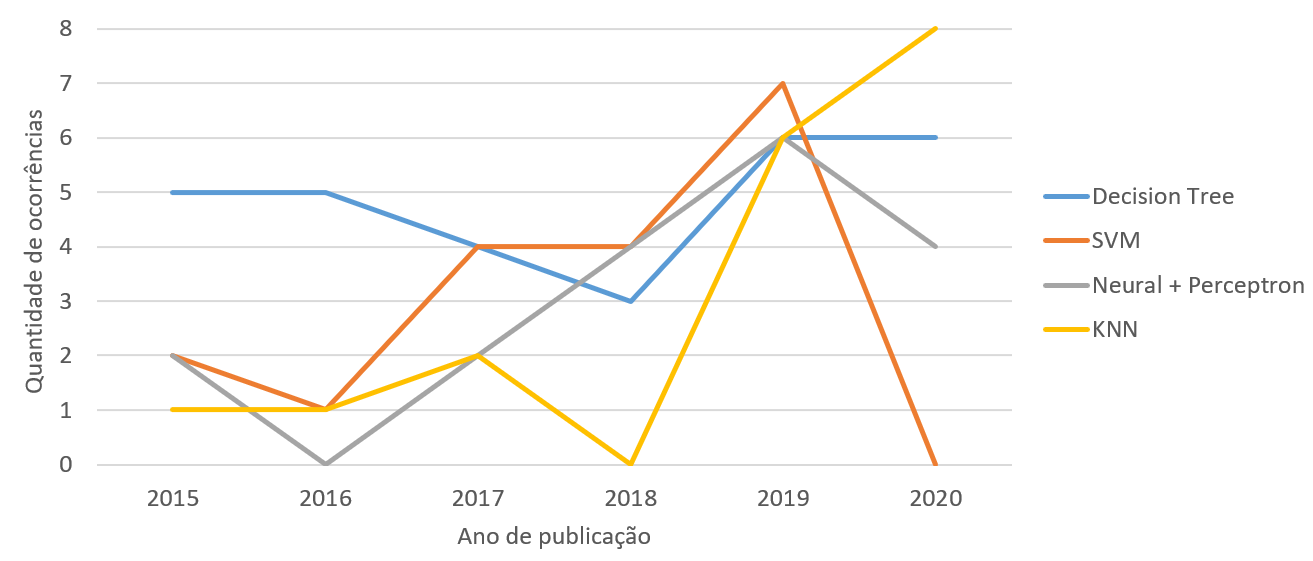
\includegraphics[width=\textwidth,keepaspectratio]{figs/tendencias_classificadores.png}
\newline \centering{ Fonte: Elaborado pelo autor.}\label{fig:tend_class}
\end{figure}

Na Figura \ref{fig:tend_Ensemble} é possível observar a variação na quantidade de ocorrências por técnicas de \textit{Ensemble} organizadas ano a ano. A estabilização da técnica \textit{random forest} nos últimos anos seguido de queda em 2020 bem como a oscilação das técnicas \textit{bagging}, \textit{boosting} e \textit{voting} as excluem como tendência para criação de um método novo de \textit{Ensemble}. Embora o uso de \textit{Stacking} em números absolutos seja o menor comparado aos demais, faz-se importante destacar o crescente uso nos últimos 4 anos. A presente pesquisa basear-se-á na técnica \textit{Stacking} para construção de um detector de intrusão. Mais detalhes sobre os principais métodos de \textit{Ensemble} na Seção \ref{Ensemble}.



\begin{figure}[H]
\centering
\caption{Técnicas de \textit{Ensemble} utilizadas - visualização ano a ano.} \includegraphics[width=\textwidth,keepaspectratio]{figs/tendencias_Ensemble.png}
\newline \centering{ Fonte: Elaborado pelo autor.}\label{fig:tend_Ensemble}
\end{figure}






\subsubsection{Métricas de desempenho - visualização dos resultados}
\label{sub-metricas}
Como forma de avaliar a eficácia dos classificadores é comum a utilização de métricas que se baseiam em valores obtidos após a construção de uma matriz que relaciona os erros e acertos do processo de classificação por parte do processo de \textit{score}. Tal matriz é denominada \textit{confusion matrix} \cite{sokolova2006beyond}. Um exemplo pode ser observado na Tabela \ref{tab:conf_matrix}:






\begin{table}[!htpb]\centering
\label{tab:conf_matrix}
\caption{Arquitetura de uma \textit{confusion matrix}. Fonte: Adaptada de \citeonline{labonne2019cascade}}.

\begin{tabular}{l|l|l}
\hline
\textbf{Classe} / \textbf{Reconhecida} & \textbf{como Positivo}       & \textbf{como Negativo}       \\ \hline \hline

Positivo             & \textit{True Positive} (TP)  & \textit{False Negative} (FN) \\ \hline
Negativo             & \textit{False Positive} (FP) & \textit{True Negative} (TN)
\\ \hline
\end{tabular}
\end{table}


No campo da detecção de intrusão os \textit{datasets} consistem de dados que representam fluxo de rede. Tais dados são pacotes que podem ser de ataques (originalmente positivo) e de tráfego legítimo benigno (originalmente negativo). Assim sendo, no processo de classificação, considera-se que:

\begin{itemize}
    \item TP: um pacote que foi classificado como ataque e que de fato era um ataque;
    \item FN: um pacote que foi classificado como benigno mas que era originalmente um pacote de ataque;
    \item FP: um pacote que era benigno originalmente mas que foi detectado como ataque, e
    \item TN: um pacote benigno que foi classificado como tal.
\end{itemize}

De forma a qualificar os trabalhos obtidos por meio de Revisão Sistemática da Literatura, as Tabelas de 10 a 14 organizam os resultados publicados pelos respectivos autores. As métricas usadas foram as expressas nas Equações de 2.1 até 2.12 detalhadas de acordo com \citeonline{das2019ddos}, \citeonline{jabbar2017cluster}, \citeonline{sokolova2006beyond} e \citeonline{sebastien2014handbook}. Os resultados são expressos por meio de \textit{detection rate} (DR), \textit{false positive rate} (FPR), \textit{false acceptance rate} (FAR), \textit{true positive rate} (TPR), \textit{false negative rate} (FNR), \textit{true negative rate} (TNR), \textit{precision} (PREC), \textit{recall} (REC), \textit{sensitivity} (SEN), \textit{specificity} (SPEC), \textit{accuracy} (ACC), F1-\textit{Score} (F1), área sob a curva ROC (AUC) e área sob a curva \textit{precision/recall} (PR AUC):

\begin{equation}
DR = \frac{TP}{TP+FN}
\end{equation}

\begin{equation}
FPR = FAR = \frac{FP}{FN + TP + TN}
\end{equation}

\begin{equation}
TPR = \frac{TP}{FN + FP + TN}
\end{equation}

\begin{equation}
FNR = \frac{FN}{TP + FP + TN}
\end{equation}

\begin{equation}
TNR = \frac{TN}{TP + FP + FN}
\end{equation}

\begin{equation}
PREC = \frac{TP}{TP + FP}
\end{equation}

\begin{equation}
REC = SENS = \frac{TP}{TP + FN}
\end{equation}

\begin{equation}
SPEC = \frac{TN}{FP + TN}
\end{equation}

\begin{equation}
ACC = \frac{TP + TN}{TP + FP + TN + FN}
\end{equation}

\begin{equation}
F1 = \left(\frac{2}{REC^{-1}+PREC^{-1}}\right)
\end{equation}

\begin{equation}
ROC AUC = \left(\frac{SENS + SPEC}{2}\right)
\end{equation}

\begin{equation}
PR AUC = \left(\frac{PREC + REC}{2}\right)
\end{equation}


Alguns artigos agrupam os resultados por tipo de ataque, por \textit{dataset}, por tipo de \textit{Ensemble} ou  por classificador. De forma a deixar a visualização dos dados mais fidedígna possível aos valores constantes das publicações original, adotou-se o seguinte esquema de organização para os resultados agrupados:

Para grupos de resultados por tipo de ataque: DoS (\textbf{A1}), Probe (\textbf{A2}), R2L (\textbf{A3}), U2R (\textbf{A4}) e pacotes benignos (\textbf{A5});

Para os diferentes \textit{datasets}: KDD Cup 1999 (\textbf{D1}), NSL-KDD	(\textbf{D2}), UNSW-NB15	(\textbf{D3}), CICIDS 2017	(\textbf{D4}), KDD-Test+	(\textbf{D5}), KDD-Test-21	(\textbf{D6}), NIMS	(\textbf{D7}), Kyoto	(\textbf{D8}), GPRS	(\textbf{D9}), ISCX	(\textbf{D10}) e HTTP CSIC 2010	(\textbf{D11});

Para os tipos de \textit{Ensemble}: Bagging	(\textbf{E1}), Boosting	(\textbf{E2}), Random Forest	(\textbf{E3}), Bagged Tree	(\textbf{E4}), Logitboost	(\textbf{E5}), Gentleboost (\textbf{E6}), Rusboost	(\textbf{E7}), Fractalboosting	(\textbf{E8}), Majority vote	(\textbf{E9}), Weighted sum	(\textbf{E10}), Rotation Forest	(\textbf{E11}) e Stacking	(\textbf{E12});

Por fim, para os diferentes classificadores: Naive Bayes	(\textbf{C1}), Decision Tree	(\textbf{C2}), Multilayer Perceptron	(\textbf{C3}), SVM	(\textbf{C4}), k-NN (\textbf{C5}), e Reptree	(\textbf{C5}).

Na sequência os resultados podem ser observados seguindo os esquemas de organização supracitados, desde as métricas de avaliação até os agrupamentos de valores. Se faz importante observar que os valores de ID constantes na primeira coluna das tabelas de resultados dizem respeito ao número do artigo, conforme elencados nas tabelas de trabalhos correlatos para os anos de 2015 a 2019 (Tabelas de 1 a 5).

As tabelas \ref{tab:result1}, \ref{tab:result2} e \ref{tab:result3} trazem as métricas de desempenho de acordo com os valores que constam nas publicações supracitadas, sendo organizadas da seguinte forma:

\begin{itemize}
    \item Tabela \ref{tab:result1} - DR, FPR, TPR, FNR e PREC;
    \item Tabela \ref{tab:result2} - REC, ACC, F1, SEM e SPEC;
    \item Tabela \ref{tab:result3} - ROC AUC, PR AUC, FAR, FP+TN e FP+FN.
\end{itemize}

% TODOS OS RESULTADOS

\begin{longtable}{l|l|l|l|l|l}
\caption{Compilação dos resultados publicados para os artigos citados (parte 1 de 3). Fonte: Elaborado pelo autor.}
\label{tab:result1}

\hline

\textbf{ID} & \textbf{DR}                                                                                                                                 & \textbf{FPR}                                                                          & \textbf{TPR}                                                                          & \textbf{FNR}                                                             & \textbf{PREC}                                                                                                \\ \hline \hline
\endfirsthead \caption[]{Continuação.} \endhead \caption[]{Fim.} \endlastfoot

1  & 0.895                                                                                                                              & 0.1                                                                          &                                                                              &                                                                 &                                                                                                     \\ \hline
2  &                                                                                                                                    & 0.021                                                                        & 0.980                                                                        &                                                                 &                                                                                                     \\ \hline

6  &                                                                                                                                    & 0.003                                                                        &                                                                              &                                                                 &                                                                                                     \\ \hline

9  &                                                                                                                                    & \begin{tabular}[c]{@{}l@{}}0.004 (E1)\\ 0.002 (E2)\end{tabular}              &                                                                              & \begin{tabular}[c]{@{}l@{}}0.035 (E1)\\ 0.017 (E2)\end{tabular} & \begin{tabular}[c]{@{}l@{}}0.992 (E1)\\ 0.996 (E2)\end{tabular}                                     \\ \hline

12 &                                                                                                                                    &                                                                              &                                                                              &                                                                 & 0.960                                                                                               \\ \hline
13 &                                                                                                                                    &                                                                              &                                                                              &                                                                 & 0.882                                                                                               \\ \hline

16 &                                                                                                                                    & 0.019                                                                        &                                                                              & 0.108                                                           &                                                                                                     \\ \hline

19 & \begin{tabular}[c]{@{}l@{}}0.504 (E9)\\ 0.773 (E10)\\ 0.841 (C1)\\ 0.771 (E1)\\ 0.767 (E2)\\ 0.697 (E11)\\ 0.801 (E3)\end{tabular} &                                                                              &                                                                              &                                                                 &                                                                                                     \\ \hline
20 & \begin{tabular}[c]{@{}l@{}}0.897 (D2)\\ 0.991 (D3)\end{tabular}                                                                    &                                                                              &                                                                              &                                                                 &                                                                                                     \\ \hline

22 & 0.910                                                                                                                              & 0.022                                                                        &                                                                              &                                                                 &                                                                                                     \\ \hline
23 &                                                                                                                                    & 0.126                                                                        &                                                                              &                                                                 &                                                                                                     \\ \hline

25 & 0.998                                                                                                                              &                                                                              &                                                                              &                                                                 &                                                                                                     \\ \hline

29 &                                                                                                                                    & \begin{tabular}[c]{@{}l@{}}0 (D2)\\ 0 (D1)\end{tabular}                      & \begin{tabular}[c]{@{}l@{}}1 (D2)\\ 1 (D1)\end{tabular}                      &                                                                 & \begin{tabular}[c]{@{}l@{}}1 (D2)\\ 0.999 (D1)\end{tabular}                                         \\ \hline
30 & 0.985                                                                                                                              & 0.420                                                                        &                                                                              &                                                                 &                                                                                                     \\ \hline
31 &                                                                                                                                    &                                                                              &                                                                              &                                                                 & \begin{tabular}[c]{@{}l@{}}0.999 (D2)\\ 1 (D10)\\ 0.999 (D11)\end{tabular}                          \\ \hline
32 & \begin{tabular}[c]{@{}l@{}}0.991 (E4)\\ 0.975 (E2)\\ 0.977 (E5)\\ 0.991 (E6)\\ 0.839 (E7)\end{tabular}                             &                                                                              &                                                                              &                                                                 &                                                                                                     \\ \hline

34 & 0.979                                                                                                                              & 0.147                                                                        &                                                                              &                                                                 & 0.930                                                                                               \\ \hline
35 & 0.985                                                                                                                              & 0.141                                                                        &                                                                              &                                                                 &                                                                                                     \\ \hline
36 &                                                                                                                                    &                                                                              &                                                                              &                                                                 & 0.996                                                                                               \\ \hline

39 &                                                                                                                                    &                                                                              &                                                                              &                                                                 & 0.999                                                                                               \\ \hline
40 &                                                                                                                                    &                                                                              &                                                                              &                                                                 & 0.960                                                                                               \\ \hline
41 & \begin{tabular}[c]{@{}l@{}}0.983 (D1)\\ 0.977 (D2)\\ 0.9992 (D8)\end{tabular}                                                      & \begin{tabular}[c]{@{}l@{}}0.032 (D1)\\ 0.024 (D2)\\ 0.017 (D8)\end{tabular} &                                                                              &                                                                 &                                                                                                     \\ \hline
43 &                                                                                                                                    &                                                                              &                                                                              &                                                                 & \begin{tabular}[c]{@{}l@{}}0.972 (D2)\\ 0.947 (D1)\\ 0.904 (D3)\\ 0.904 (D3)\end{tabular}           \\ \hline
44 & 0.997                                                                                                                              &                                                                              &                                                                              &                                                                 &                                                                                                     \\ \hline
46 &                                                                                                                                    &                                                                              &                                                                              &                                                                 & \begin{tabular}[c]{@{}l@{}}0.976 (A5)\\ 0.985 (A1)\\ 0.757 (A2)\\ 0.991 (A3)\\ 0.692 (A4)\end{tabular} \\ \hline
47 &                                                                                                                                    & \begin{tabular}[c]{@{}l@{}}0.142 (E2)\\ 0.057 (E3)\\ 0.057 (E1)\end{tabular} & \begin{tabular}[c]{@{}l@{}}0.903 (E2)\\ 0.902 (E3)\\ 0.901 (E1)\end{tabular} &                                                                 &                                                                                                     \\ \hline
48 &                                                                                                                                    &                                                                              &                                                                              &                                                                 &                                                                                                     \\ \hline
49 & \begin{tabular}[c]{@{}l@{}}0.970 (D3)\\ 0.973 (D7)\end{tabular}                                                                    & \begin{tabular}[c]{@{}l@{}}0.025 (D3)\\ 0.041 (D7)\end{tabular}              &                                                                              &                                                                 &                                                                                                     \\ \hline
50 &                                                                                                                                    & \begin{tabular}[c]{@{}l@{}}0.014 (D1)\\ 0.034 (D2)\end{tabular}              & \begin{tabular}[c]{@{}l@{}}0.702 (D1)\\ 0.742 (D2)\end{tabular}              &                                                                 &                                                                                                     \\ \hline
51 & 0.990                                                                                                                              &                                                                              &                                                                              &                                                                 &                                                                                                     \\ \hline
52 &                                                                                                                                    &                                                                              &                                                                              &                                                                 & 0.864                                                                                               \\ \hline
53 &                                                                                                                                    &                                                                              &                                                                              &                                                                 & 0.783                                                                                               \\ \hline
54 &                                                                                                                                    &                                                                              &                                                                              &                                                                 & 0.999                                                                                               \\ \hline
55 & 0.997                                                                                                                              & 0.230                                                                        &                                                                              &                                                                 &                                                                                                     \\ \hline
57 & \begin{tabular}[c]{@{}l@{}}1 (D1)\\ 0.998 (D2)\\ 0.974 (D3)\\ 0.999 (D3)\end{tabular}                                              &                                                                              &                                                                              &                                                                 &                                                                                                     \\ \hline
60 &                                                                                                                                    &                                                                              &                                                                              &                                                                 & \begin{tabular}[c]{@{}l@{}}0.929 (D2)\\ 0.933 (D3)\end{tabular}                                     \\ \hline
61 &                                                                                                                                    & \begin{tabular}[c]{@{}l@{}}0.117 (D5)\\ 0.089 (D6)\\ 0.063 (D3)\end{tabular} &                                                                              &                                                                 & \begin{tabular}[c]{@{}l@{}}0.880 (D5)\\ 0.916 (D6)\\ 0.916 (D3)\end{tabular}                          
\\ \hline

62 &
&
&
&
&
\begin{tabular}[c]{@{}l@{}}0.980 (D2)\\ 1.0 (D3)\end{tabular}
\\ \hline



63 &
&
&
&
&
\begin{tabular}[c]{@{}l@{}}0.725 (E9)\\ 0.771 (E1)\\ 0.786 (E3)\\ 0.785 (E2)\end{tabular}
\\ \hline



68 &
&
&
&
&
\begin{tabular}[c]{@{}l@{}}0.90 (A5)\\ 
0.790 (A2)\\ 
0.940 (A1)\\
0.150 (A3)\\
0.490 (A4)\\
\end{tabular}
\\ \hline





\end{longtable}







\begin{longtable}{l|l|l|l|l|l}
\caption{Compilação dos resultados publicados para os artigos citados (parte 2 de 3). Fonte: Elaborado pelo autor.}
\label{tab:result2}

\hline
\textbf{ID} & \textbf{REC}                                                                                                     & \textbf{ACC}                                                                                                                                                                                                                                       & \textbf{F1}                                                                                                     & \textbf{SEM}                                                                                                    & \textbf{SPE}                                                                                                 \\ \hline \hline
\endfirsthead \caption[]{Continuação.} \endhead \caption[]{Fim.} \endlastfoot


3  &                                                                                                         &                                                                                                                                                                                                                                           & 0.98                                                                                                   &                                                                                                        &                                                                                                     \\ \hline
4  &                                                                                                         & \begin{tabular}[c]{@{}l@{}}0.987 (A1)\\ 0.987 (A2)\\ 0.981 (A3)\\ 0.984 (A4)\end{tabular}                                                                                                                                                 &                                                                                                        &                                                                                                        &                                                                                                     \\ \hline
5  &                                                                                                         &                                                                                                                                                                                                                                           &                                                                                                        & \begin{tabular}[c]{@{}l@{}}0.760 (C1)\\ 0.065 (C2)\\ 0.760 (C4)\\ 0.756 (C5)\\ 0.685 (C6)\end{tabular} & \begin{tabular}[c]{@{}l@{}}0.990 (C1)\\ 0.989 (C2)\\ 0.989 (C4)\\ 0.986 (C5)\\ 0.989 (C6)\end{tabular} \\ \hline
6  &                                                                                                         & 0.996                                                                                                                                                                                                                                     &                                                                                                        &                                                                                                        &                                                                                                     \\ \hline
7  &                                                                                                         & 0.978                                                                                                                                                                                                                                     &                                                                                                        &                                                                                                        &                                                                                                     \\ \hline
8  &                                                                                                         & 0.973                                                                                                                                                                                                                                     &                                                                                                        &                                                                                                        &                                                                                                     \\ \hline
9  & \begin{tabular}[c]{@{}l@{}}0.964 (E1)\\ 0.982 (E2)\end{tabular}                                         &                                                                                                                                                                                                                                           &                                                                                                        &                                                                                                        &                                                                                                     \\ \hline
11 &                                                                                                         & 0.9997                                                                                                                                                                                                                                    &                                                                                                        &                                                                                                        &                                                                                                     \\ \hline
12 & 0.960                                                                                                   & 0.963                                                                                                                                                                                                                                     &                                                                                                        &                                                                                                        &                                                                                                     \\ \hline
13 & 0.807                                                                                                   &                                                                                                                                                                                                                                           &                                                                                                        &                                                                                                        &                                                                                                     \\ \hline
15 &                                                                                                         & 0.994                                                                                                                                                                                                                                     &                                                                                                        &                                                                                                        &                                                                                                     \\ \hline
16 &                                                                                                         & 0.921                                                                                                                                                                                                                                     &                                                                                                        &                                                                                                        &                                                                                                     \\ \hline
20 &                                                                                                         & \begin{tabular}[c]{@{}l@{}}0.903 (D2)\\ 0.994 (D3)\end{tabular}                                                                                                                                                                           &                                                                                                        &                                                                                                        &                                                                                                     \\ \hline
21 &                                                                                                         & \begin{tabular}[c]{@{}l@{}}*aprox.:\\ 0.970 (A2)\\ 0.975 (A1)\\ 0.990 (A4)\\ 0.860 (A3)\end{tabular}                                                                                                                                      &                                                                                                        &                                                                                                        &                                                                                                     \\ \hline
23 &                                                                                                         & 0.850                                                                                                                                                                                                                                     &                                                                                                        &                                                                                                        &                                                                                                     \\ \hline
24 &                                                                                                         & \begin{tabular}[c]{@{}l@{}}0.995 (D2)\\ 0.955 (D3)\\ 0.918 (D9)\end{tabular}                                                                                                                                                              &                                                                                                        &                                                                                                        &                                                                                                     \\ \hline
25 &                                                                                                         & 0.9993                                                                                                                                                                                                                                    &                                                                                                        &                                                                                                        &                                                                                                     \\ \hline
26 &                                                                                                         & 0.900                                                                                                                                                                                                                                     &                                                                                                        &                                                                                                        &                                                                                                     \\ \hline
28 &                                                                                                         & \begin{tabular}[c]{@{}l@{}}0.832 (E1+C1)\\ 0.817 (E1+C3)\\ 0.867 (E1+C2)\\ 0.868 (E1+C5)\\ 0.852 (E2+C1)\\ 0.810 (E2+C3)\\ 0.868 (E2+C2)\\ 0.865 (E2+C5)\\ 0.847 (E12+C1)\\ 0.832 (E12+C3)\\ 0.871 (E12+C2)\\ 0.879 (E12+C5)\end{tabular} &                                                                                                        &                                                                                                        &                                                                                                     \\ \hline
30 &                                                                                                         &                                                                                                                                                                                                                                           & 0.960                                                                                                  &                                                                                                        &                                                                                                     \\ \hline
31 & \begin{tabular}[c]{@{}l@{}}0.998 (D2)\\ 1 (D10)\\ 0.998 (D11)\end{tabular}                              & \begin{tabular}[c]{@{}l@{}}0.9995 (D2)\\ 1 (D10)\\ 0.9998 (D11)\end{tabular}                                                                                                                                                              & \begin{tabular}[c]{@{}l@{}}0.998 (D2)\\ 1 (D10)\\ 0.998 (D11)\end{tabular}                             &                                                                                                        &                                                                                                        \\ \hline

33 &                                                                                                         & 0.878                                                                                                                                                                                                                                     &                                                                                                        &                                                                                                        &                                                                                                     \\ \hline
34 & 0.920                                                                                                   & 0.924                                                                                                                                                                                                                                     & 0.936                                                                                                  &                                                                                                        &                                                                                                     \\ \hline
35 &                                                                                                         & 0.882                                                                                                                                                                                                                                     &                                                                                                        &                                                                                                        &                                                                                                     \\ \hline
36 & 0.972                                                                                                   & 0.949                                                                                                                                                                                                                                     &                                                                                                        &                                                                                                        &                                                                                                     \\ \hline
37 &                                                                                                         & \begin{tabular}[c]{@{}l@{}}0.931 (A2)\\ 0.112 (A3)\\ 0.254 (A4)\\ 0.994 (A5)\end{tabular}                                                                                                                                                 &                                                                                                        &                                                                                                        &                                                                                                     \\ \hline
38 &                                                                                                         & 0.845                                                                                                                                                                                                                                     &                                                                                                        &                                                                                                        &                                                                                                     \\ \hline
39 & 0.9998                                                                                                  & 0.9997                                                                                                                                                                                                                                    &                                                                                                        &                                                                                                        &                                                                                                     \\ \hline
40 & 0.960                                                                                                   & 0.958                                                                                                                                                                                                                                     & 0.950                                                                                                  &                                                                                                        &                                                                                                     \\ \hline
41 &                                                                                                         & \begin{tabular}[c]{@{}l@{}}0.989 (D1)\\ 0.974 (D2)\\ 0.991 (D8)\end{tabular}                                                                                                                                                              &                                                                                                        &                                                                                                        &                                                                                                     \\ \hline
42 &                                                                                                         & 0.961                                                                                                                                                                                                                                     &                                                                                                        &                                                                                                        &                                                                                                     \\ \hline
43 & \begin{tabular}[c]{@{}l@{}}0.921 (D2)\\ 0.998 (D1)\\ 0.972 (D3)\\ 0.956 (D3)\end{tabular}               &                                                                                                                                                                                                                                           & \begin{tabular}[c]{@{}l@{}}0.946 (D2)\\ 0.972 (D1)\\ 0.937 (D3)\\ 0.929 (D3)\end{tabular}              &                                                                                                        &                                                                                                     \\ \hline
45 &                                                                                                         & 0.842                                                                                                                                                                                                                                     &                                                                                                        &                                                                                                        &                                                                                                     \\ \hline
46 & \begin{tabular}[c]{@{}l@{}}0.9996 (A5)\\ 0.991 (A1)\\ 0.995 (A2)\\ 0.971 (A3)\\ 0.890 (A4)\end{tabular} &                                                                                                                                                                                                                                           & \begin{tabular}[c]{@{}l@{}}0.989 (A5)\\ 0.988 (A1)\\ 0.860 (A2)\\ 0.981 (A3)\\ 0.778 (A4)\end{tabular} &                                                                                                        &                                                                                                     \\ \hline
49 &                                                                                                         & \begin{tabular}[c]{@{}l@{}}0.989 (D3)\\ 0.982 (D7)\end{tabular}                                                                                                                                                                           &                                                                                                        &                                                                                                        &                                                                                                     \\ \hline
50 &                                                                                                         & \begin{tabular}[c]{@{}l@{}}0.977 (D1)\\ 0.952 (D2)\end{tabular}                                                                                                                                                                           & \begin{tabular}[c]{@{}l@{}}0.071 (D1)\\ 0.720 (D2)\end{tabular}                                        &                                                                                                        &                                                                                                     \\ \hline
51 &                                                                                                         & 0.994                                                                                                                                                                                                                                     &                                                                                                        &                                                                                                        &                                                                                                     \\ \hline
52 & 0.842                                                                                                   & 0.842                                                                                                                                                                                                                                     & 0.836                                                                                                  &                                                                                                        &                                                                                                     \\ \hline
53 & 0.911                                                                                                   & 0.822                                                                                                                                                                                                                                     & 0.842                                                                                                  &                                                                                                        &                                                                                                     \\ \hline
54 & 0.999                                                                                                   & 0.999                                                                                                                                                                                                                                     &                                                                                                        &                                                                                                        &                                                                                                     \\ \hline
56 &                                                                                                         & 0.994                                                                                                                                                                                                                                     &                                                                                                        &                                                                                                        &                                                                                                     \\ \hline
57 &                                                                                                         & \begin{tabular}[c]{@{}l@{}}0.9997 (D1)\\ 0.998 (D2)\\ 0.958 (D3)\\ 0.998 (D3)\end{tabular}                                                                                                                                                &                                                                                                        &                                                                                                        &                                                                                                     \\ \hline
58 &                                                                                                         & \begin{tabular}[c]{@{}l@{}}0.980 (A5)\\ 0.953 (A1)\\ 0.911 (A2)\\ 0.552 (A3)\\ 0.142 (A4)\end{tabular}                                                                                                                                    &                                                                                                        &                                                                                                        &                                                                                                     \\ \hline
59 &                                                                                                         & 0.848                                                                                                                                                                                                                                     &                                                                                                        &                                                                                                        &                                                                                                     \\ \hline
60 & \begin{tabular}[c]{@{}l@{}}0.924 (D2)\\ 0.917 (D3)\end{tabular}                                         & \begin{tabular}[c]{@{}l@{}}0.917 (D2)\\ 0.918 (D3)\end{tabular}                                                                                                                                                                           &                                                                                                        &                                                                                                        &                                                                                                     \\ \hline
61 &                                                                                                         & \begin{tabular}[c]{@{}l@{}}0.857 (D5)\\ 0.725 (D6)\\ 0.912 (D3)\end{tabular}                                                                                                                                                              &                                                                                                        & \begin{tabular}[c]{@{}l@{}}0.868 (D5)\\ 0.913 (D6)\\ 0.913 (D3)\end{tabular}                           &  \\ \hline                                                                                             




62 &
\begin{tabular}[c]{@{}l@{}}0.970 (D2)\\
1 (D4) \end{tabular} & 

\begin{tabular}[c]{@{}l@{}}0.975 (D2)
\\ 0.9968 (D4) \end{tabular} & 

\begin{tabular}[c]{@{}l@{}}0.970 (D2)\\
1 (D4) \end{tabular} & & \\ 
\hline





63 & & 
\begin{tabular}[c]{@{}l@{}}0.812 (E9)
\\ 0.854 (E1)
\\ 0.863 (E3)
\\ 0.865 (E2) \end{tabular} & 

\begin{tabular}[c]{@{}l@{}}0.820 (E9)
\\ 0.847 (E1)
\\ 0.857 (E3)
\\ 0.858 (E2) \end{tabular} & &

\hline

64 & & 0.9856 & & & \hline
65 & & 0.9941 & & & \hline



67 & & \begin{tabular}[c]{@{}l@{}}0.9998 (D4)
\\ 0.985 (D11)
\\ 0.921 (D2)
\\ 0.936 (D3) \end{tabular} & & & \hline



\end{longtable}
















\begin{longtable}{l|l|l|l|l|l}
\caption{Compilação dos resultados publicados para os artigos citados (parte 3 de 3). Fonte: Elaborado pelo autor.}
\label{tab:result3}

\hline

\textbf{ID} & \textbf{ROC AUC}                                                                                                & \textbf{PR AUC}                                                                                    & \textbf{FAR}                                                                                   & \textbf{FP+TN}                                                                                                                              & \textbf{FP+FN}                                                                                                                           \\ \hline \hline
\endfirsthead \caption[]{Continuação.} \endhead \caption[]{Fim.} \endlastfoot
2  & 0.996                                                                                                  &                                                                                           &                                                                                       &                                                                                                                                    &                                                                                                                                 \\ \hline
13 &                                                                                                        & 0.890                                                                                     &                                                                                       &                                                                                                                                    &                                                                                                                                 \\ \hline
14 &                                                                                                        & 0.960                                                                                     &                                                                                       &                                                                                                                                    &                                                                                                                                 \\ \hline
18 &                                                                                                        & \begin{tabular}[c]{@{}l@{}}1 (A1)\\ 0.999 (A2)\\ 0.995 (A3)\\ 0.999 (A4)\end{tabular}     &                                                                                       &                                                                                                                                    &                                                                                                                                 \\ \hline
19 &                                                                                                        &                                                                                           &                                                                                       & \begin{tabular}[c]{@{}l@{}}0.495 (E9)\\ 0.226 (E10)\\ 0.158 (C1)\\ 0.228 (E1)\\ 0.232 (E2)\\ 0.302 (E11)\\ 0.198 (E3)\end{tabular} & \begin{tabular}[c]{@{}l@{}}0.495 (E9)\\ 0.226 (E10)\\ 0.158 (C1)\\ 0.228 (E1)\\ 0.232 (E2)\\ 0.302 (E11)\\ 0.198 (E3)\end{tabular} \\
20 &                                                                                                        &                                                                                           & \begin{tabular}[c]{@{}l@{}}0.082 (D2)\\ 0.180 (D3)\end{tabular}                       &                                                                                                                                    &                                                                                                                                 \\ \hline
24 &                                                                                                        &                                                                                           & \begin{tabular}[c]{@{}l@{}}0.003 (D2)\\ 0.072 (D3)\\ 0.063 (D9)\end{tabular}          &                                                                                                                                    &                                                                                                                                 \\ \hline
25 &                                                                                                        &                                                                                           & 0.0003                                                                                &                                                                                                                                    &                                                                                                                                 \\ \hline
32 & \begin{tabular}[c]{@{}l@{}}0.963 (E4)\\ 0.954 (E2)\\ 0.968 (E5)\\ 0.972 (E6)\\ 0.950 (E7)\end{tabular} &                                                                                           &                                                                                       &                                                                                                                                    &                                                                                                                                 \\ \hline
34 &                                                                                                        & 0.916                                                                                     &                                                                                       &                                                                                                                                    &                                                                                                                                 \\ \hline
38 &                                                                                                        &                                                                                           & 0.531                                                                                 &                                                                                                                                    &                                                                                                                                 \\ \hline
43 &                                                                                                        & \begin{tabular}[c]{@{}l@{}}0.985 (D2)\\ 0.984 (D1)\\ 0.980 (D3)\\ 0.963 (D3)\end{tabular} &                                                                                       &                                                                                                                                    &                                                                                                                                 \\ \hline
45 &                                                                                                        &                                                                                           & 0.027                                                                                 &                                                                                                                                    &                                                                                                                                 \\ \hline
47 & \begin{tabular}[c]{@{}l@{}}0.951 (E2)\\ 0.981 (E3)\\ 0.952 (E1)\end{tabular}                           &                                                                                           &                                                                                       &                                                                                                                                    &                                                                                                                                 \\ \hline
50 & \begin{tabular}[c]{@{}l@{}}0.844 (D1)\\ 0.855 (D2)\end{tabular}                                        &                                                                                           &                                                                                       &                                                                                                                                    &                                                                                                                                 \\ \hline
51 &                                                                                                        &                                                                                           & 0.110                                                                                 &                                                                                                                                    &                                                                                                                                 \\ \hline
53 &                                                                                                        &                                                                                           & 0.272                                                                                 &                                                                                                                                    &                                                                                                                                 \\ \hline
57 &                                                                                                        &                                                                                           & \begin{tabular}[c]{@{}l@{}}0 (D1)\\ 0.001 (D2)\\ 0.069 (D3)\\ 0.002 (D3)\end{tabular} &                                                                                                                                    &                                                                                                                                 \\ \hline
\end{longtable}
















\section{Sistemas de Detecção de Intrusão}

\label{sec:ids}

De acordo com \citeonline{osken2019intrusion}, as ações relacionadas com foco na manutenção da integridade, acessibilidade ou confiabilidade de uma fonte de dados eletrônicos ou de uma rede de comunicação definem os objetivos de um IDS. Os autores fazem uma leitura histórica do surgimento e da evolução dos IDS atribuindo a James Anderson - quando da publicação do artigo ``\textit{Computer Security Threat Monitoring and Surveillance}'', por \citeonline{anderson1980computer}, o primeiro relato de um IDS. Dois fatos marcantes na evolução dos IDS ocorreram em 1986 e posteriormente em 1993 quando publicações documentavam cientificamente modelos de detecção de intrusão baseados em análises estatísticas do tráfego de rede (ambos criados por Dorothy Denning e Peter Neumann em \citeonline{denning1987intrusion}).

\citeonline{karatas2018neural} definem um IDS como um software desenvolvido para detectar ataques que tenham potencial para causar danos na rede de comunicação ou nos sistemas, sejam eles provenientes de um meio inseguro como a Internet ou da rede local. Tais softwares executam contramedidas de segurança ao detectar alguma anomalia no tráfego de rede ou no comportamento dos hosts que possa caracterizar um ataque.

Os autores destacam que recentemente muitas abordagens têm sido aplicadas para se aumentar a taxa de detecção, de forma geral, envolvendo técnicas de \textit{Machine Learning} (situações onde o detector aprende por meio de treinamento a detectar anomalias), \textit{Rule Based} (caso onde o detector possui assinaturas características de ataques e apenas compara o tráfego real com as assinaturas de ataques já conhecidos) e/ou métodos estatísticos clássicos (emprego de cálculos de média, desvio padrão, mediana, dentre outros).

\citeonline{stallings2016network} destaca que a aplicação de um modelo de detecção de intrusão somente é possível caso o comportamento dos usuários possa ser caracterizado em ``legítimo'' ou ``abusivo''. Contudo, em muitos cenários não existe um limite exato de comportamento, conforme a Figura \ref{fig:pdf} ilustra.

% figura pdf
\begin{figure}
\centering
\caption{Funções Densidade de Probabilidade para Comportamentos Mensuráveis.} 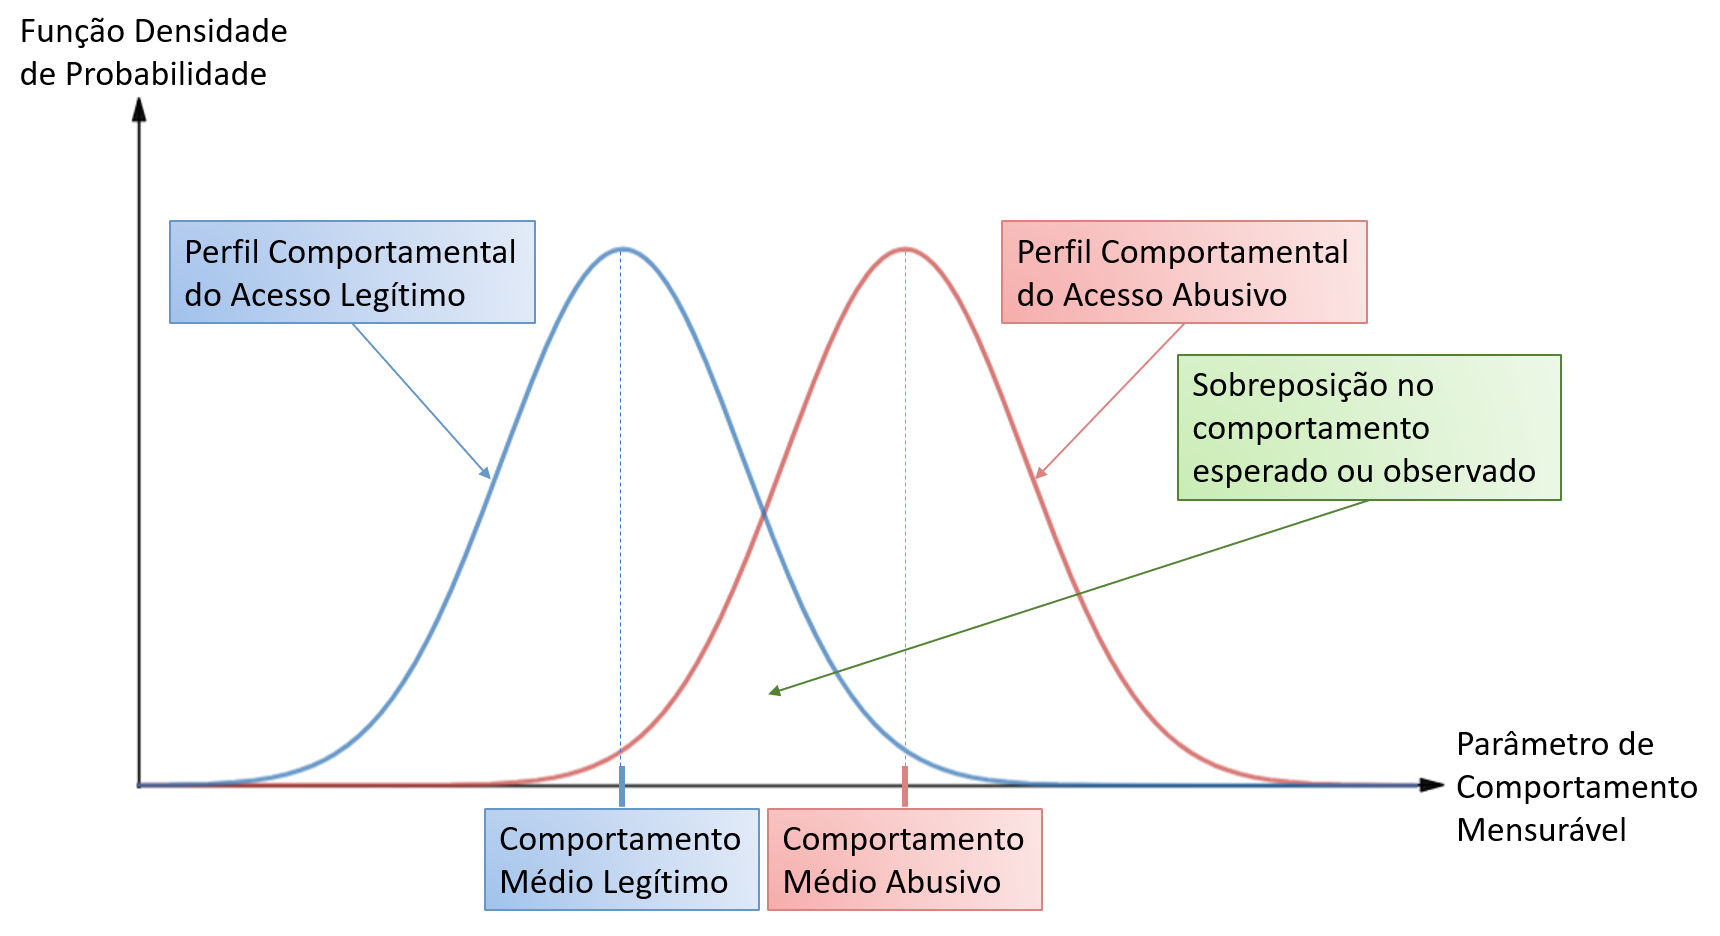
\includegraphics[width=12cm,height=\textwidth,keepaspectratio]{figs/funcao_densidade_probabilidade.png}
\newline \centering{Fonte: Elaborado pelo Autor. Adaptado de \citeonline{stallings2016network}.}\label{fig:pdf}
\end{figure}

As curvas gaussianas (Figura \ref{fig:pdf}) ilustram, à esquerda, a distribuição normal de determinado comportamento mensurável que caracteriza usuários legítimos e, à direita, na mesma lógica, um perfil de comportamento abusivo. Entretanto, no caso exposto, existe uma sobreposição entre as duas distribuições normais que eleva o grau de dificuldade na classificação do comportamento. Técnicas mais robustas de classificação tendem a apresentar uma taxa de acurácia mais próxima da realidade com altos índices de \textit{true-positives} (situação onde um acesso legítimo ou abusivo é classificado corretamente) enquanto técnicas menos apuradas tendem a aumentar as taxas de \textit{false-negatives} (quando os rótulos são atribuídos de forma incorreta). 

Os IDS possuem duas dimensões de classificação: pela Topologia de Rede e pela Abordagem dos Pacotes. A primeira dimensão, de acordo com \citeonline{kaouk2019review}, define se o detector trabalha analisando o fluxo de rede (topologicamente, neste caso, o IDS normalmente é colocado na rede de comunicação em forma de \textit{bridge}\footnote{situação topológica onde o dispositivo de rede é o único meio pelo qual o tráfego ocorre.} ou recebendo uma cópia de todos os pacotes trafegados por meio de espelhamento\footnote{técnica utilizada para se enviar cópias dos \textit{frames} de outras portas para uma porta específica onde o IDS será conectado.} de uma porta da \textit{switch}\footnote{dispositivo de interconexão de redes atuante na camada de Enlace do modelo de referência OSI.}) ou analisando o comportamento do sistema operacional, situação onde o detector trabalha observando medidas de processamento, espaço em disco, uso de memória ou auditando registros feitos nos logs do sistema. Já a segunda dimensão de classificação diz respeito a maneira como o detector analisa os dados. \citeonline{ran2019semi} afirmam que nesta categorização existem duas classes: detecção por assinatura ou detecção por anomalia. Os autores explicam que na detecção por assinatura o IDS possui uma base de dados de ataques já conhecidos e basicamente seu trabalho é comparar os pacotes que chegam até a rede com o seu banco de dados de forma a verificar similaridades. Na detecção por anomalia, entretanto, o sistema define um modelo de que seria o comportamento ``normal'' da rede ou do sistema fazendo com que pacotes que não se classifiquem como ``normais'' sejam rotulados como maliciosos.


As próximas Subseções documentam com maiores detalhes as categorias de classificação dos IDS, sendo eles: Classificação pela Topologia da Rede (  \ref{subsec:topologia}) e Classificação pela Abordagem dos Pacotes (\ref{subsec:abordagem}).









\subsection{Classificação pela Topologia da Rede}
\label{subsec:topologia}


Conforme já observado, os IDS podem ser divididos em dois grupos: \textit{Host Based} IDS (HIDS) e \textit{Network Based} IDS (NIDS). \citeonline{alam2019collaborative} destacam que os HIDS trabalham analisando o comportamento do sistema operacional de forma a detectar anomalias, enquanto os NIDS trabalham analisando o tráfego de rede. A Figura \ref{fig:nids_hids} ilustra as diferenças topológicas entre estas duas abordagens:

% figura hids nids
\begin{figure}[H]
\centering
\caption{Comparação entre HIDS e NIDS.} 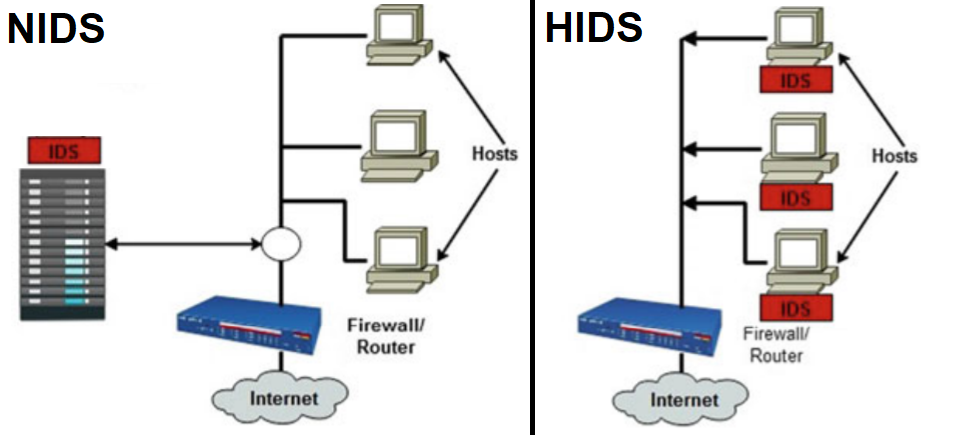
\includegraphics[width=12cm,height=\textwidth,keepaspectratio]{figs/hids_nids.png}
\newline \centering{ Fonte: Adaptado de  \citeonline{deb2019wi}}\label{fig:nids_hids}
\end{figure}

Na Figura \ref{fig:nids_hids} é possível observar que a rede à esquerda possui um ``IDS \textit{System}'' responsável por analisar todo o tráfego de rede proveniente e com destino para a Internet, enquanto que na topologia à direita existe, para cada host na rede, um IDS responsável por monitorá-lo.

Um exemplo prático de aplicação de um HIDS pode ser ilustrado por um hipotético servidor de arquivos FTP\footnote{Protocolo da camada de aplicação do modelo OSI utilizado para transferência de arquivos.} que gera e armazena registros de todas as autenticações e transações em um arquivo de logs. Um HIDS, neste caso, poderia monitorar tal arquivo de logs das autenticações e, caso detecte que num período curto de tempo o mesmo host falhou em autenticar muitas vezes (um caso de ataque de \textit{bruteforce}\footnote{Ataque baseado em tentativa e erro onde o atacante procura conseguir as credenciais de acesso válidas por meio de uso de dicionários}.), poderia bloquear o endereço IP do host atacante ou alertar o administrador do sistema para que determinada providência seja tomada. Já um exemplo de aplicação de um NIDS pode ser observado na presença de um sistema detector de intrusão hipotético que receba cópias de todos os pacotes que trafegam pela rede e os analise em busca de comportamentos anômalos. Caso perceba que determinada anatomia do tráfego caracteriza um ataque, o NIDS pode bloqueá-lo ou alertar o responsável humano pelo sistema.















\subsection{Classificação pela Abordagem dos Pacotes}
\label{subsec:abordagem}


De acordo com \citeonline{li2019enabling} os IDS também podem ser classificados de acordo com o método usado para determinar o tipo de ataque, sendo eles ``Baseados em Assinatura'' ou ``Baseados em Anomalia''. A Figura \ref{fig:assinatura} ilustra o método de funcionamento dos IDS Baseados em Assinatura: 

% figura assinatura
\begin{figure}[H]
\centering
\caption{Fluxo de funcionamento na Detecção por Assinatura.} 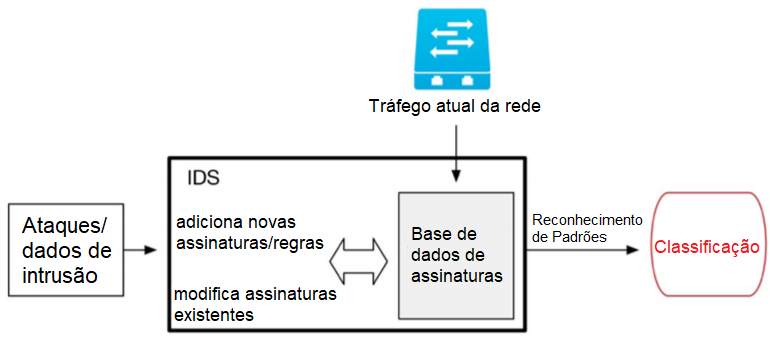
\includegraphics[width=12cm,height=\textwidth,keepaspectratio]{figs/assinatura.png}
\newline \centering{ Fonte:  Adaptado de \citeonline{li2019enabling}}\label{fig:assinatura}
\end{figure}

Nestes cenários o detector conhece a anatomia de vários tipos de ataques, pois mantém uma base de dados com a assinatura de diversos tráfegos conhecidamente maliciosos. \citeonline{datir2019survey} documentam que os IDS baseados em assinatura possuem como principal desvantagem o fato de só detectarem ataques previamente conhecidos, entretanto conseguem entregar uma boa taxa de detecção com baixo número de alarmes \textit{false-negatives}.

A Figura \ref{fig:anomalia} ilustra o método de funcionamento dos Sistemas Baseados em Anomalia:

%figura anomalia
\begin{figure}[H]
\centering
\caption{Fluxo de funcionamento na Detecção por Anomalia.} 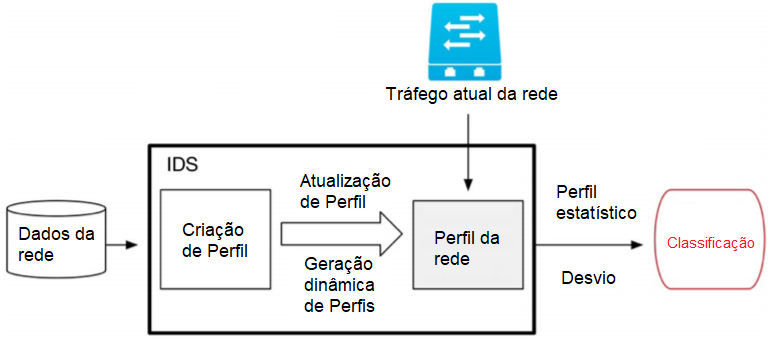
\includegraphics[width=12cm,height=\textwidth,keepaspectratio]{figs/anomalia.png}
\newline \centering{ Fonte:  Adaptado de \citeonline{li2019enabling}}\label{fig:anomalia}
\end{figure}

Nos Sistemas Baseados em Anomalia cabe ao administrador da rede determinar baseado em seu conhecimento empírico o que é um tráfego legítimo e o que não é. \citeonline{datir2019survey} afirmam que uma vantagem significativa dos IDS baseados em anomalia é a capacidade de detectar ataques desconhecidos pois observam um desvio no comportamento normal da rede ou do sistema, porém caso a atividade maliciosa não se enquadre como abusiva no método de classificação o ataque será rotulado como acesso legítimo, o que ocasiona a diminuição na acurácia da detecção uma vez que a taxa de \textit{false-negatives} tende a aumentar.


















% \section{Sistemas de Detecção de Intrusão \textit{Open Source}}
% \label{sec:ids_opensource}
% Snort, Suricata e Bro (também pode ser encontrado na literatura como ``Zeek'') são os IDS \textit{open source} mais utilizados de acordo com \citeonline{AT&TCybersecurity}, \citeonline{wong2017enhancing} e  \citeonline{bhosale2015comparative}. O presente tópico caracteriza tais softwares de forma a documentar seu funcionamento destacando os principais pontos positivos e negativos. Uma taxonomia dos IDS elencados pode ser observada na Tabela \ref{tab:ids_opensource}.

% \subsection{Snort}

% \citeonline{goel2019implementation} afirmam que o Snort pode atuar com regras padrão, obtidas via pacote de instalação ou pela comunidade, ou ainda trabalhar com regras escritas pelo próprio administrador da rede de comunicação e dos sistemas. Os autores destacam a capacidade de Snort em detectar e previnir ataques de diferentes tipos. 

% A infraestrutura do Snort, ainda de acordo com os autores, consiste em codificação criada na linguagem C por Martin Roesch e sua equipe que na época (1998–2013) pertenciam à Sourcefire, empresa que mais tarde (2013) viria a ser adquirida pela Cisco. 

% Destacam-se, em relação ao Snort, a grande quantidade de implementações em redes e citações em artigos científicos, é o que documentam  \citeonline{shah2018performance}. Os autores detalham o fluxo de funcionamento no processo de detecção do Snort que consiste nas etapas de:

% \begin{itemize}
    
%     \item Recepção dos pacotes provenientes de um \textit{Network Backbone} por meio do módulo de captura de pacotes denominado \textit{Sniffer};
    
%     \item Pré-processamento dos pacotes para que sejam extraídos dados relevantes ao processo de classificação;
    
%     \item Comparação dos pacotes recebidos com os alarmes já conhecidos (assinaturas presentes na base de dados [\textit{Rulesets}]);
    
%     \item Etapa de decisão sendo possível o envio de alertas e/ou apenas o a execução do processo de \textit{logging} que irá armazenar informações de classificação para fins estatísticos ou de forense\footnote{Ciência que compreende o uso de ferramentas, técnicas e métodos para se desvendar um ataque ou um crime}. 
% \end{itemize}

% O fluxo sistemático exposto é ilustrado na Figura \ref{fig:fluxograma-snort}:

% % figura snort fluxograma
% \begin{figure}[H]
% \centering
% \caption{} 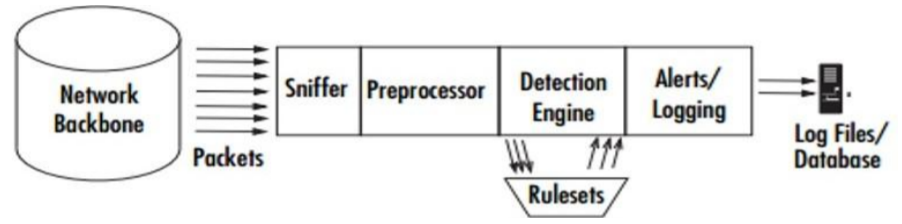
\includegraphics[width=12cm,height=\textwidth,keepaspectratio]{figs/fluxograma-snort.png}
% \caption{Fluxo de funcionamento do Snort. Fonte: \citeonline{shah2018performance}.}\label{fig:fluxograma-snort}
% \end{figure}

% \citeonline{cui2018research} além de enfatizarem o já exposto por  \citeonline{shah2018performance} (que documenta a larga utilização do Snort no processo de detecção de intrusão), destacam o fato do detector ser de livre distribuição e de código-fonte aberto. Também enfatizam ser um software leve para execução por ser baseado na biblioteca libpcap\footnote{Biblioteca de programação aberta que permite ter acesso aos pacotes que trafegam pela rede de comunicação}.


% \subsection{Suricata}

% O Suricata surgiu com o propósito de substituir o Snort. É o que afirmam \citeonline{sheikh2018lightweight}. Os autores ainda destacam o fato do Suricata possuir suporte à múltiplos processadores (\textit{multi-threaded}), diferentemente do Snort, o que torna a taxa de processamento dos pacotes mais efetivo fazendo com que o número de \textit{dropped packets}\footnote{Pacotes não processados pelo detector em virtude da capacidade de processamento ser menor do que o fluxo de dados} caia consideravelmente. Uma outra virtude relevante do Suricata em relação ao Snort é conseguir detectar segmentos TCP\footnote{Protocolo da camada de transporte do modelo OSI responsável por adicionar controle e confiabilidade aos datagramas IP, além de informar via cabeçalho o número das portas de origem e destino referentes ao serviço da camada de aplicação} e datagramas UDP\footnote{Protocolo da camada de transporte do modelo OSI responsável por informar via cabeçalho o número das portas de origem e destino referentes ao serviço da camada de aplicação} mesmo que o número da porta utilizada esteja fora do padrão de numeração determinado pelo IETF\footnote{Mais detalhes na RFC-1700 <https://tools.ietf.org/html/rfc1700>}. 

% A escalabilidade do Suricata é destacada por  \citeonline{beraldo2018analise} no tocante à capacidade de distribuição da carga de processamento em cada um dos processadores do detector de intrusão. Os autores também destacam que a capacidade do Suricata em detectar os fluxos mais comuns torna-o um excelente detector de \textit{malwares}\footnote{Categorização geral dos softwares com objetivos maliciosos.}. Ainda de acordo com os autores, o Suricata possui a funcionalidade de reconhecer extensões de arquivos em fluxo na rede e gravar uma cópia em disco para análise de \textit{hash}\footnote{Sequência de caracteres gerados por um algoritmo de criptografia que tem por função atestar a integridade de um determinado dado.} em tempo real. Em resumo, caso o \textit{hash} calculado pertença a alguma \textit{blacklist}\footnote{Lista de termos proibidos geralmente usada para controle de acesso em redes de comunicação.} previamente gerada, o detector conseguirá bloquear a entrada de tal arquivo na rede.

% O fluxo sistemático de trabalho do Suricata pode ser observado na Figura \ref{fig:fluxograma-suricata}:

% % figura suricata fluxograma
% \begin{figure}[H]
% \centering
% \caption{} \includegraphics[width=12cm,height=\textwidth,keepaspectratio]{figs/fluxograma-suricata.png}
% \caption{Fluxo de funcionamento do Suricata. Fonte: \citeonline{shah2018performance}.}\label{fig:fluxograma-suricata}
% \end{figure}

% Com base na Figura \ref{fig:fluxograma-suricata} pode-se interpretar o funcionamento lógico do Suricata como segue:

% \begin{itemize}

%     \item Aquisição dos pacotes provenientes da rede a ser monitorada;
    
%     \item Pré-processamento (camada de decodificação) para que sejam extraídos dados relevantes dos pacotes;
    
%     \item Diversos módulos de detecção que ilustram a capacidade \textit{multi-thread} do Suricata. Tais módulos irão aplicar a detecção por assinaturas conhecidas;
    
%     \item Etapa de saída, onde um classificador binário irá afirmar se os pacotes analisados são característicos de um ataque ou de um arquivo malicioso (ou não), ou um classificador multiclasse irá determinar o tipo de ataque dentre os vários conhecidos por meio das assinaturas. 


% \end{itemize}

 
 



% \subsection{BRO}

% \citeonline{bdair2020brief} afirmam que o IDS BRO (que pode também ser conhecido como ``Zeek'') tem por objetivo monitorar comportamentos suspeitos na rede e é distribuído como software \textit{open source}. Embora o IDS tenha suporte à IPv6, por características gerais das regras da versão mais nova do Protocolo de Internet, apresenta baixa acurácia quando habilitado a monitorar tal protocolo. \citeonline{singh2018security} complementam a caracterização do BRO afirmando que o detector baseado em Unix\footnote{Sistema operacional multitarefa e multiusuário criado por pesquisadores da AT&T em 1965.} é capaz de prover bons resultados no monitoramento em tempo real do fluxo por conta da sua capacidade de realizar análises detalhadas (\textit{deep scanning}) dos pacotes que trafegam pela rede. 

% Uma análise mais abrangente do BRO é apresentada por  \citeonline{beraldo2018analise} que o categoriza como um NIDS capaz de entregar bons resultados tanto em ambientes acadêmicos (criados para fins científicos) ou no mercado (ambiente real de produção), o que tem feito seu emprego nas redes crescer consideravelmente. Os autores destacam o fato da comunidade de suporte do BRO ser bastante completa sendo composta por grandes universidades, laboratórios de pesquisa, centros de supercomputação e a própria comunidade \textit{open source}. Um ponto interessante do BRO é a sua capacidade de implementação em redes SDN. Por possuir uma linguagem de programação orientada à redes, as suas implementações permitem abstrair as ideias dos fluxos, onde os pacotes são agrupados por endereço, porta de origem e porta de destino. Um diferencial relevante do BRO é que além de detector ele pode ser considerado um caracterizador de fluxos, resumindo as informações do tráfego de rede e agrupando as informações por intervalos de tempo, permitindo análises diversas por parte dos administradores da rede e dos sistemas. 

% A Figura \ref{fig:fluxograma-bro} apresenta o fluxo lógico de funcionamento do BRO: 

% % figura suricata fluxograma
% \begin{figure}[H]
% \centering
% \caption{} 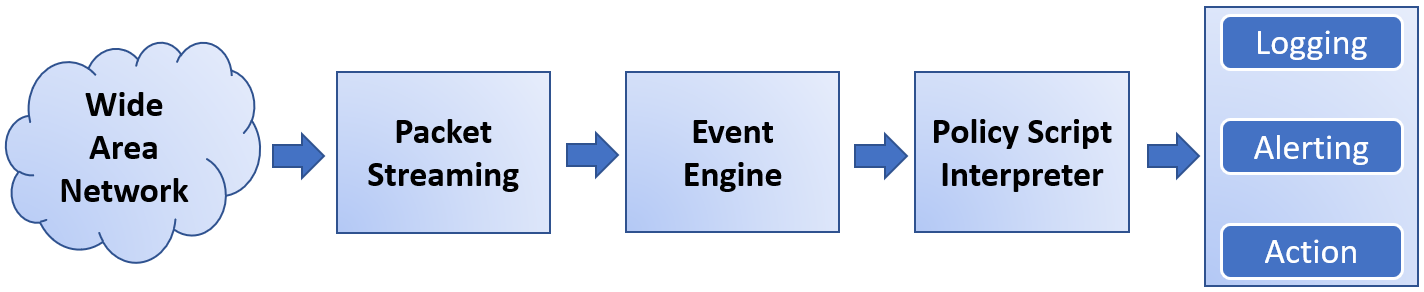
\includegraphics[width=12cm,height=\textwidth,keepaspectratio]{figs/fluxograma-bro.png}
% \caption{Fluxo de funcionamento do BRO. Fonte: Elaborado pelo autor. Adaptado de  \citeonline{singh2018security}.}\label{fig:fluxograma-bro}
% \end{figure}

% A sistemática apresentada na Figura \ref{fig:fluxograma-bro} pode ser interpretada como segue:

% \begin{itemize}

%     \item Os pacotes provenientes da rede a ser monitorada são recepcionados pelo módulo \textit{Packet Streaming} que é responsável por processá-los e repassar apenas dados relevantes adiante;
    
%     \item O módulo \textit{Event Engine} é responsável por validar a integridade dos pacotes recebidos por meio de funções \textit{hash};
    
%     \item O \textit{Policy Script Interpreter} é quem irá aplicar as regras e os scripts tendo como objeto de análise os pacotes recebidos e então, de acordo com a configuração prévia, determinar se será feito \textit{Logging} (apenas a guarda dos registros), \textit{Alerting} (envio de notificação ao administrador da rede ou dos sistemas alertando a detecção de anomalias) ou/e \textit{Action} (bloqueio do provável atacante na rede). 
    
    
    
    
% \end{itemize}




% \subsection{Análise Comparativa entre Snort, Suricata e BRO}
% \label{sec:tax_idsopen}


% Embora Snort, Suricata e BRO tenham o mesmo objetivo geral  (detectar anomalias na rede) cada um dos softwares possui particularidades de implementação, o que entrega ao administrador da rede ou dos sistemas vantagens e desvantagens em relação ao uso dos softwares. \citeonline{isa2019comprehensive} realizaram um estudo comparativo entre os principais detalhes funcionais dos IDS citados que podem ser resumidos, em seus pontos principais, como pode ser observado na Tabela \ref{tab:ids_opensource}:

% \begin{longtable}{c|c|c|c|c|c|c|c}
%     \caption{Taxonomia dos IDS \textit{Open Source} citados no tópico. Elaborado pelo Autor. Adaptado de \citeonline{isa2019comprehensive}.}
%     \label{tab:ids_opensource}

% %\begin{tabular}
%     \hline
%     \textbf{IDS} & \textbf{UMR} & \textbf{TDP} & \textbf{MP} & \textbf{PI} & \textbf{DOC} & \textbf{CSO}\\
%     \hline
%     \hline
    
    
%     \textbf{Snort} &
%     Média &
%     Alta\footnote{Apresentada quando o Snort está em execução em grandes redes} &
%     Não &
%     Sim &
%     Completa  &
%     Multiplataforma \\
%     \hline
    
    
%     \textbf{Suricata} &
%     Alta &
%     Média &
%     Sim &
%     Sim &
%     Completa  &
%     Windows, Unix e MacOS    \\
%     \hline
    
    
%     \textbf{BRO} &
%     Baixa &
%     Baixa &
%     Sim &
%     Sim &
%     Incompleta  &
%     Linux, FreeBSD e MacOS    \\
%     \hline
    
% \end{longtable}

% A taxonomia exposta na Tabela \ref{tab:ids_opensource} caracteriza os IDS \textit{Open Source} de acordo com a Utilização de Memória RAM (UMR); a Taxa de \textit{Dropped Packets} (TDP); se o sistema tem a capacidade de execução em múltipos processadores (MP); se é capaz de, além de detectar, previnir intrusões (PI); como a documentação oficial disponível foi avaliada; e a compatibilidade do IDS entre os Sistemas Operacionais (CSO). 









\section{\textit{Data Mining} em \textit{Datasets}} 

\label{sec:datamining}

Muitos esforços têm sido empregados na criação de modelos de detecção de intrusão baseados em \textit{Data Mining}. Alguns \textit{datasets} têm sido usados para tal. A presente Seção tem como objetivo descrever brevemente os \textit{datasets} mais comuns em estudos científicos por meio de uma breve revisão da literatura. 

\subsection{Visão Geral}
Os dados contidos nos \textit{datasets} são, basicamente, pacotes provenientes de fluxo legítimo (benígnos) e outros provenientes de ataques (maliciosos). Esta seção busca fazer uma análise das publicações que sustentam as principais bases de dados e que permite elencar a relação de ataques de cada um dos \textit{datasets}:

De acordo com \citeonline{kolias2015intrusion}, o \textit{dataset} ``AWID'' contempla ataques típicos de redes 802.11\footnote{Tecnologia de redes sem fio (Wi-Fi) especificada pela IEEE.}.

\citeonline{santanna2015booters} destacam que o \textit{dataset} ``Booters'' possui dados característicos de nove tipos de ataques DDoS. Outra base de ataques de negação de serviços é a publicada por \citeonline{alkasassbeh2016detecting}, ``DDoS 2016''.

A base de dados ``Botnet'' possui ataques provenientes de diversas redes de computadores zumbis\footnote{Hosts infectados por meio de malwares que são controlados remotamente por atacantes.} segundo \citeonline{beigi2014towards}. O \textit{dataset} publicado por \citeonline{garcia2014empirical}, ``CTU-13'' segue a mesma linha, bem como a base de dados ``ISOT'' de autoria de \citeonline{saad2011detecting}.

\citeonline{jazi2017detecting} destacam que a base de dados ``CIC DoS'' contempla pacotes de ataques de negação de serviço direcionados à camada de aplicação do modelo OSI.  

\citeonline{sharafaldin2018toward} fornecem no \textit{dataset} ``CICIDS-2017'' uma coletânea de ataques que incluem dados provenientes de \textit{botnets}\footnote{Uma rede de hosts infectados que é controlada remotamente por atacantes}, ataques de XSS\footnote{Ataque onde páginas maliciosas executam código arbitrário no cliente web}, DoS\footnote{Ataque um único host malicioso envia requisições em larga escala com o objetivo de esgotar a capacidade de processamento do alvo}, DDoS, \textit{heartbleed}\footnote{Vulnerabilidade na biblioteca OpenSSL que pode dar acesso à chaves privadas de criptografia ao atacante.}, SSH\footnote{Protocolo da camada de aplicação do modelo OSI que fornece acesso remoto à máquinas que possuam servidor SSH}, SQL \textit{injection}\footnote{Situação onde o atacante consegue injetar queries SQL nas requisições web com o objetivo de ter acesso ou modificar algum registro em um banco de dados.}, dentre outros.

O \textit{dataset} fornecido por \citeonline{ring2017creation}, ``CIDDS-001'' possui dados de DoS, \textit{port scan}\footnote{Ataque onde é possível obter a anatomia da vítima por meio de scripts que informam as portas e os serviços disponíveis no alvo.} e SSH \textit{brute force}. Em uma publicação posterior, \citeonline{ring2019flow} forneceu no \textit{dataset} ``CIDDS-002'' uma sequência mais detalhada contemplando apenas ataques de \textit{port scans}, de forma similar à anatomia do \textit{dataset} ``LBNL'' fornecido por \citeonline{pang2006devil}.

O banco de dados ``DARPA'', de acordo com \citeonline{lippmann2000evaluating} traz ataques de DoS, \textit{privilege escalation}\footnote{Ataque onde, de posse das credenciais de acesso de um usuário simples, o atacante consegue acesso administrativo (root).} e \textit{port scans}.

\citeonline{shiravi2012toward} documentam que o \textit{dataset} ``ISCX 2012'' contempla dados de DoS, DDoS, SSH \textit{brute force} e cenários onde há ataques provenientes da rede interna.

O \textit{dataset} ``KDD Cup 1999'' \citeonline{KDDCUP} contempla dados de DoS, \textit{privilege escalation} e \textit{port scans}.

A base de dados publicada por \citeonline{song2011statistical}, ``Kioto 2006+'', contempla uma variedade de ataques coletados por \textit{honeypots}\footnote{Servidores propositalmente vulneráveis que têm por objetivo coletar dados de ataques} como \textit{backscatter}\footnote{Ataque onde os endereços IP de origem dos pacotes maliciosos são falsificados gerando respostas para hosts aleatórios}, DoS, \textit{exploits}\footnote{Códigos maliciosos com objetivo de explorar vulnerabilidades específicas.}, \textit{malware}, \textit{port scans} e \textit{shellcode}\footnote{Similar aos \textit{exploits}, buscam explorar vulnerabilidades específicas}. \citeonline{sperotto2009hidden} também publicaram um \textit{dataset} baseado em dados coletados por \textit{honeypots} denominado ``Twente'', com foco específico em ataques a servidores FTP, HTTP e SSH.

A base de dados ``NDSec-1'' fornecida por \citeonline{beer2017new} é bastante variada e contém dados de ataques de \textit{brute force}, \textit{botnet}, DDoS, \textit{exploits}, \textit{port scans}, \textit{spoofing}\footnote{Ataque onde busca-se fraudar algum host na rede fazendo-no crer que o atacante é um host confiável com quem ele pode se comunicar}, XSS, SQL \textit{injection}, dentre outros.

Os \textit{datasets} ``NSL-KDD'' e ``PU-IDS'' de autoria de \citeonline{tavallaee2009detailed} e \citeonline{singh2015reference}, respectivamente, possuem dados de DoS, \textit{privilege escalation} e \textit{port scans}.

\citeonline{sharma2018new} publicaram o \textit{dataset} ``PUF'' que contém variados dados de ataques a servidores DNS. De forma análoga, \citeonline{hofstede2014ssh} publicaram o \textit{dataset} ``SSHCure'' que contém variados ataques a servidores SSH.

\citeonline{wheelus2014session} por meio do \textit{dataset} ``SANTA'' fornecem dados de vários tipos de ataques, como DoS, DDoS, DNS \textit{amplification}\footnote{Ataque de negação de serviço que tem como alvo servidores de nomes.}, \textit{heartbleed} e \textit{port scans}.

A base de dados ``SSENET-2011'' de \citeonline{vasudevan2011ssenet} também fornece vários dados de diversos tipos de ataques como DoS, \textit{port scans} e uma gama de scripts maliciosos executados via Metasploit\footnote{Coletânea de softwares para geração de ataques.}. Uma versão mais nova da base citada foi denominada ``SSENET-2014'' e publicada por \citeonline{bhattacharya2014ssenet} contempla dados de ataques \textit{flooding}, \textit{botnets}, \textit{privilege escalation} e \textit{port scans}.

O \textit{dataset} ``TRAbID'' de autoria de \citeonline{viegas2017toward} contém dados de ataques DoS e \textit{port scans}.

\citeonline{goel2019implementation} publicaram a base de dados ``TUIDS'' que traz dados de ataques provenientes de \textit{botnets}, DDoS, \textit{port scans} e SSH \textit{brute force}.

O \textit{dataset} ``UGR'16'' publicado por \citeonline{macia2018ugr} documenta ataques provenientes de \textit{botnets}, DoS, \textit{port scan}, SSH \textit{brute force} e spam\footnote{Mensagens enviadas para destinatários arbitrártios sem que estes tenham-nas solicitadas}.

\citeonline{moustafa2015unsw} publicaram o ``UNSW-NB15'' que contempla vários ataques como DoS, \textit{exploits}, \textit{backdoors}, \textit{portscans}, \textit{shellcode}, spams e \textit{malwares}.

\citeonline{sangster2009toward}, \citeonline{zuech2015new}, \citeonline{kent2015comprehensive_a}, \citeonline{kent2016cyber},  \citeonline{gringoli2009gt} e \citeonline{turcotte2017unified} não forneceram detalhes acerca da tipologia dos ataques presentes em seus \textit{datasets}.

\subsection{Taxonomia dos \textit{Datasets} de Intrusão}
\label{tax_datasets}
Uma compilação baseada em \citeonline{ring2019survey} resultou na Tabela \ref{tab:datasets} onde é possível observar detalhes como o nome do \textit{dataset}, os autores responsáveis pela sua publicação, o tipo da rede usada para criação, o tipo do trafego e o tamanho da base de dados fornecida. Os colunas ``TR'', ``TT'', ``TD'' e ``L'' significam, respectivamente, ``Tamanho da Rede'', ``Tipo do Tráfego'', ``Tamanho do \textit{Dataset}'' (que pode ser especificado em \textit{packages}, \textit{flows} ou \textit{points} de acordo com o método escolhido para especificar o tamanho pelos autores) e ``\textit{Labeled}'' (se os dados são rotulados):



\begin{longtable}{c|c|c|c|c|c}
    \caption{Resumo dos \textit{Datasets} de Intrusão Comumente Utilizados para \textit{Data Mining}. Adaptado de \citeonline{ring2019survey}}
    \label{tab:datasets}

%\begin{tabular}
    \hline
    \textbf{Dataset} & Autor(es) & \textbf{TR} & \textbf{TT} & \textbf{TD} & \textbf{L} \\
    \hline
    \hline
    \endfirsthead \caption[]{Continuação.} \endhead \caption[]{Fim.} \endlastfoot
    
    
    AWID &
    \citeonline{kolias2015intrusion} &
    pequena &
    emulado &
    37 MB  &
    S \\
    \hline
    
    
    Booters &
     \citeonline{santanna2015booters} &
    pequena &
    real &
    250 GB  &
    N    \\
    \hline
    
    
    Botnet &
     \citeonline{beigi2014towards} &
    diversificada &
    emulado &
    14 GB  &
    S    \\
    \hline
    
    
    CIC DoS &
     \citeonline{jazi2017detecting} &
    pequena &
    emulado &
    4.6 GB  &
    S    \\
    \hline
    
    
    CICIDS-2017 &
     \citeonline{sharafaldin2018toward} &
    pequena &
    emulado &
    3.1 MB  &
    S    \\
    \hline
    
    
    CIDDS-001 &
     \citeonline{ring2017creation} &
    pequena &
    heterogêneo &
    32 MB  &
    S    \\
    \hline
    
    CIDDS-002 &
     \citeonline{ring2019flow} &
    pequena &
    heterogêneo &
    15 MB  &
    S    \\
    \hline
    
    
    CDX  &
    \citeonline{sangster2009toward} &
    pequena &
    real &
    14 GB  &
    N    \\
    \hline
    
    
    CTU-13 &
     \citeonline{garcia2014empirical} &
    universidade &
    real &
    81 MB  &
    S    \\
    \hline
    
    
    DARPA &
     \citeonline{lippmann2000evaluating} &
    pequena &
    emulado &
    -    &
    S \\
    \hline
    
    
    DDoS 2016 &
     \citeonline{alkasassbeh2016detecting} &
    - &
    sintético &
    21 MB  &
    S    \\
    \hline
    
    
    IRSC  &
    \citeonline{zuech2015new} &
    - &
    real &
    -    &
    S  \\
    \hline
    
    
    ISCX 2012 &
     \citeonline{shiravi2012toward} &
    pequena &
    emulado &
    2 MB   &
    S   \\
    \hline
    
    
    ISOT  &
    \citeonline{saad2011detecting} &
    pequena &
    emulado &
    11 GB   &
    S   \\
    \hline
    
    
    KDD-CUP-99 &
     \citeonline{KDDCUP} &
    pequena &
    emulado &
    5 MB   &
    S   \\
    \hline
    
    
    Kent 2016 &
     \citeonline{kent2015comprehensive_a},\citeonline{kent2016cyber} &
    empresarial &
    real &
    130 MB   &
    N   \\
    \hline
    

    Kyoto 2006+ &
     \citeonline{song2011statistical} &
    \textit{honeypots} &
    real &
    93 MB     &
    S \\
    \hline
    
    
    LBNL  &
    \citeonline{pang2006devil} &
    empresarial &
    real &
    160 MB  &
    N    \\
    \hline
    
    
    NDSec-1  &
    \citeonline{beer2017new} &
    pequena &
    emulado &
    3.5 MB   &
    S   \\
    \hline
    
    
    NGIDS-DS &
     \citeonline{haider2017generating} &
    pequena &
    emulado &
    1 MB   &
    S   \\
    \hline
        
    
    NSL-KDD &
     \citeonline{tavallaee2009detailed} &
    pequena &
    emulado &
    150 kB   &
    S   \\
    \hline
        
    
    PU-IDS  &
    \citeonline{singh2015reference} &
    pequena &
    sintético &
    200 kB    &
    S  \\
    \hline
        
    
    PUF  &
    \citeonline{sharma2018new} &
    universidade &
    real &
    300 kB   &
    S   \\
    \hline
        
    
    SANTA  &
    \citeonline{wheelus2014session} &
    ISP\footnote{Provedor de serviços que comercializam links de acesso à Internet (popularmente conhecido como ``Provedor de Internet'').} &
    real &
    -    &
    S  \\
    \hline
        
    
    SSENET-2011  &
    \citeonline{vasudevan2011ssenet} &
    pequena &
    emulado &
    -    &
    S  \\
    \hline
        
    
    SSENET-2014  &
    \citeonline{bhattacharya2014ssenet} &
    pequena &
    emulado &
    200 kB   &
    S   \\
    \hline
        
    
    SSHCure  &
    \citeonline{hofstede2014ssh} &
    universidade &
    real &
    2.4 GB    &
    S  \\
    \hline
        
    
    TRAbID  &
    \citeonline{viegas2017toward} &
    pequena &
    emulado &
    460 MB   &
    S   \\
    \hline
        
    
    TUIDS  &
    \citeonline{gogoi2012packet} &
    média &
    emulado &
    250 kB   &
    S   \\
    \hline
        
    
    Twente &
     \citeonline{sperotto2009hidden} &
    honeypot &
    real &
    14 MB   &
    S   \\
    \hline
        
    
    UGR’16 &
     \citeonline{macia2018ugr} &
    ISP &
    real &
    16.9 GB  &
    S   \\
    \hline
        
    
    UNIBS  &
    \citeonline{gringoli2009gt} &
    universidade &
    real &
    79 kB    &
    N  \\
    \hline
    
    UHN  &
    \citeonline{turcotte2017unified} &
    empresarial &
    real &
    150 GB    &
    N  \\
    \hline
    
    
    UNSW-NB15 &
     \citeonline{moustafa2015unsw} &
    pequena &
    emulado &
    2 MB   &
    S   \\
    \hline
    
    
%       \end{tabular}
\end{longtable}
    
    
\subsection{Derivações e Combinações entre os \textit{Datasets}}

Alguns \textit{datasets} apresentados são frutos de derivações ou composições de outras bases de dados. A Figura \ref{fig:datasets_comparacoes} ilustra, frente aos dados expostos na Tabela \ref{tab:datasets}, o relacionamento entre alguns \textit{datasets}, suas derivações e combinações. Em azul constam os \textit{datasets} baseados integralmente em outro e, em laranja, \textit{datasets} baseados parcialmente em outros:

% figura compara datasets
\begin{figure}[H]
\centering
\caption{Derivações e Combinações entre os Datasets.} 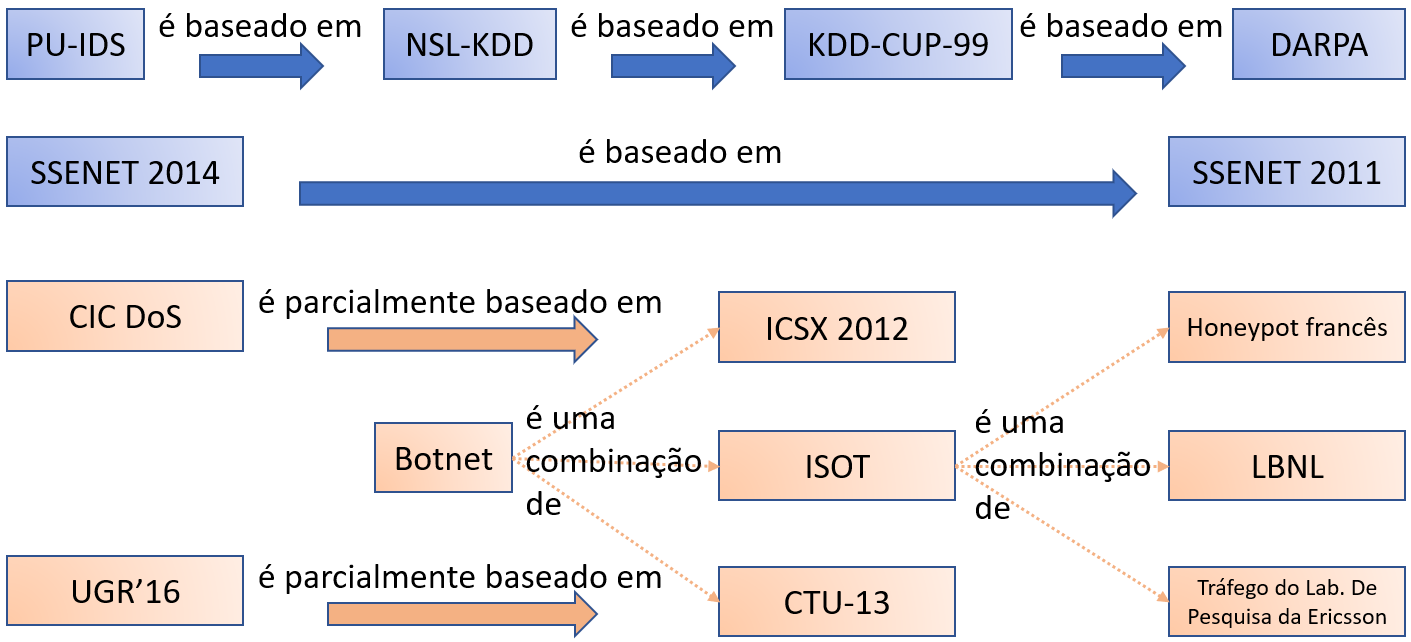
\includegraphics[width=16cm,height=\textwidth,keepaspectratio]{figs/datasets_combinacoes_derivacoes.png}
\newline \centering{ Fonte: Elaborado pelo Autor. Adaptado de  \citeonline{ring2019survey}}.\label{fig:datasets_comparacoes}
\end{figure}


A quantidade dos dados presentes nos \textit{datasets} supracitados é considerável, bem como a complexidade da anatomia dos pacotes que trafegam pelas redes, sejam eles provenientes de usuários legítimos ou de atacantes. Encontrar padrões nos dados é fundamental para que se possa tomar decisões acertadas. A busca de padrões é um desafio da Ciência dos Dados que estuda técnicas de \textit{Data Mining}. Aprender padrões para classificar dados futuros é um campo de desafio da área da Inteligência Artificial que vem empregando técnicas de \textit{Machine Learning} para classificar com cada vez mais acurácia dados futuros com base em comportamentos passados. A Seção \ref{sec:machinelearning} trata da teoria geral do assunto.




\section{\textit{Machine Learning}}
\label{sec:machinelearning}


Em termos gerais, \textit{Machine Learning} (ou Aprendizagem de Máquina) é uma linha da Inteligência Artificial pertencente à Ciência da Computação que busca, por métodos matemáticos e estatísticos e em conjunto com áreas correlatas (como, por exemplo, a própria Inteligência Artificial, Processamento de Imagens Digitais, Reconhecimento de Padrões) analisar um banco de dados (\textit{dataset}) e aprender padrões de como classificar os dados, seja por meio de classificação, agrupamento (\textit{clustering}) ou de regressão (buscar padrões lineares nos dados). Existem muitos algoritmos empregados para resolver problemas de classificação e regressão. O objetivo específico desta seção é prover uma revisão breve dos métodos de aprendizagem sem foco específico na arquitetura dos algoritmos comumente utilizados na literatura recente.

\citeonline{lee2019python} destaca a capacidade dos métodos de \textit{Machine Learning} em resolver problemas de classificação, regressão e \textit{clustering}:

\subsection{Classificação, Regressão e \textit{Clustering}}

Classificação, Regressão e \textit{Clustering} são problemas que, de acordo com o já citado 
\citeonline{lee2019python}, os algoritmos de \textit{Machine Learning}, em termos gerais, resolvem bem. 

\citeonline{bakshi2018considerations} definem que ``classificação'' consiste em treinar um algoritmo de aprendizagem em uma amostra de testes (uma porção do \textit{dataset} com dados em quantidade variável) e testá-lo na porção restante dos dados para averiguar o desempenho do algoritmo. Nas palavras de \citeonline{lee2019python}, nos problemas de classificação os algoritmos de \textit{Machine Learning} aprendem padrões nos dados presentes na amostragem de treinamento e devem ser capazes de identificar as classes às quais os dados da amostragem de testes pertencem. Ainda de acordo com o autor, ``regressão'' consiste em encontrar um padrão linear na distribuição de dados em um \textit{dataset} e é útil para prever valores. O autor finaliza definindo ``\textit{clustering}'' como um meio de agrupar dados semelhantes de acordo com determinada(s) característica(s). 

O padrão aprendido pelo algoritmo pode ser classificado como \textit{underfitting}, bom ou \textit{overfitting}, como pode-se observar na Figura \ref{fig:scikit}:

% figura scikit
\begin{figure}[H]
\centering
\caption{Qualidades de Aprendizado.} 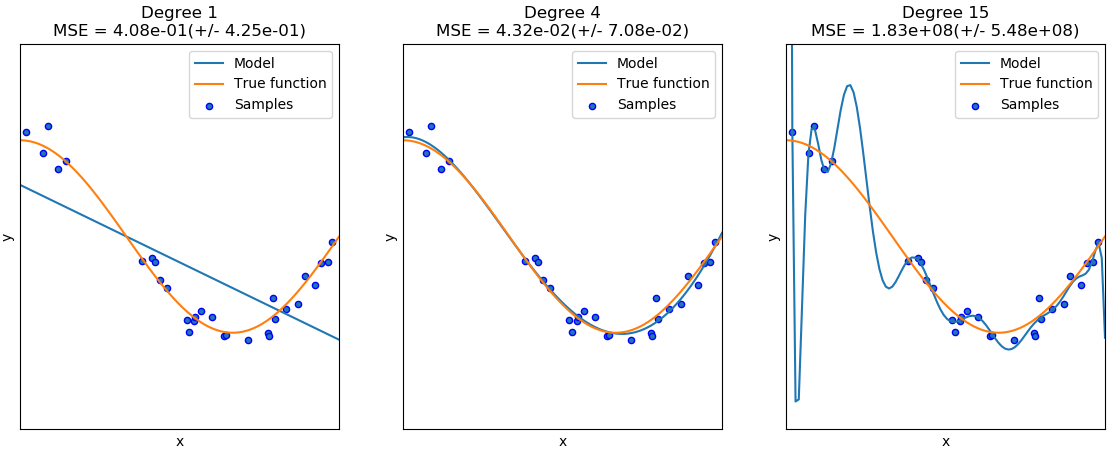
\includegraphics[width=15cm,height=\textwidth,keepaspectratio]{figs/treinamento_scikit.png}
\newline \centering{ Fonte:  \citeonline{Underfit90:online}}\label{fig:scikit}
\end{figure}

Os pontos nos três quadros ilustrados na Figura \ref{fig:scikit} são dados presentes em um \textit{dataset} hipotético. Percebe-se na situação à esquerda que o modelo aprendido tem pouca semelhança com a função de dispersão dos dados, uma situação de \textit{underfitting}. No quadro à direita há uma situação de \textit{overfitting} e o método provavelmente não será capaz de detectar outros pontos pertencentes à mesma classe pois seu aprendizado está voltado ao modelo de testes sem considerar desvios eventuais. Já no quadro central percebe-se uma situação de bom aprendizado uma vez que a função de dispersão dos dados possui pouco desvio do modelo aprendido.

\subsection{Métodos de Aprendizagem}

Os dados (seja na amostragem de treinamento ou de testes) podem ser rotulados ou não (os rótulos definem as classes às quais os dados pertencem), definindo o tipo de aprendizagem a ser implementada. Destacam-se aqui os tipos de aprendizagem presentes na literatura.




% \citeonline{geron2019hands}
% \citeonline{forsythapplied}
% \citeonline{lee2019python}


Métodos de Aprendizagem Supervisionada consistem em treinar algoritmos de forma com que os dados a serem analisados na amostragem de treinamento possuam rótulos definidos. 

De acordo com \citeonline{geron2019hands}, os métodos de aprendizagem supervisionada podem ser úteis para classificação e regressão. O autor destaca alguns exemplos de algoritmos geralmente usados em métodos supervisionados como k-NN, Regressão Linear e Logística, SVM, \textit{Decision Trees},  \textit{Random Forest} e Redes Neurais.

\citeonline{lee2019python} destaca quanto ao método de funcionamento das técnicas de aprendizagem supervisionada que os rótulos das classes presentes na amostragem de treinamento são úteis para ensinar o algoritmo sobre os padrões de todas as classes (o problema nesse ponto pode variar entre ``classificação binária'', que é quando só existem dois rótulos ou ``classificação multiclasse'', que é quando existem mais de dois rótulos) de forma com que seja possível atribuir prováveis rótulos aos dados da amostragem de testes.


Já em se tratando de métodos não-supervisionados, \citeonline{lee2019python} afirma que nestas situações os dados de treinamento não possuem rótulos e a classificação ou \textit{clustering} dos dados deve ser feita considerando \textit{features} específicas que possam agrupar dados semelhantes:



% figura unsuper
\begin{figure}[H]
\centering
\caption{Casos de Treinamento Não-Supervisionado.} 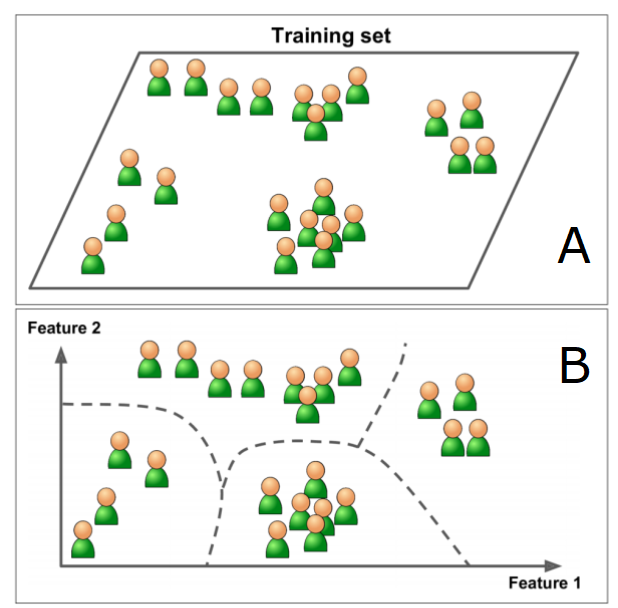
\includegraphics[width=15cm,height=10cm,keepaspectratio]{figs/unsuper.png}
\newline \centering{Fonte:  Adaptado de  \citeonline{geron2019hands}}\label{fig:unsuper}
\end{figure}

 A Figura \ref{fig:unsuper} ilustra a situação citada de forma a destacar que no quadro ``A'' percebe-se uma amostragem de treinamento onde os dados são iguais visualmente apresentando um cenário não-rotulado. O método aprendido foi capaz de, no quadro ``B'', criar linhas que dividam os dados em grupos específicos. 

De acordo com \citeonline{geron2019hands} são algoritmos típicos para solução de problemas não-supervisionados K-Means e DBSCAN para \textit{clustering} e PCA para redução da dimensionalidade de um \textit{dataset} (método normalmente usado para garantir menos dimensões de processamento).

Métodos de aprendizagem semi-supervisionados partem do princípio de que existem, num mesmo \textit{dataset}, dados que possuem rótulos e dados que não possuem \cite{li2018semi}. De acordo com \citeonline{geron2019hands} são algoritmos típicos para estes cenários as \textit{Deep Beliefs Networks}.

Por fim, na aprendizagem por reforço, de forma resumida, a saída ótima que o algoritmo busca são obtidas por meio de tentativa e erro. Para cada erro de classificação o algoritmo é penalizado. \citeonline{botvinick2019reinforcement} destacam que este tipo de método tem como desvantagem a grande quantidade de dados necessária para que exista uma boa solução de classificação.

\section{\textit{Ensemble Learning}}
\label{Ensemble}
Métodos de \textit{Ensemble Machine Learning}, de acordo com \citeonline{zhou2012Ensemble}, consistem na aplicação conjunta de diferentes algoritmos de classificação ou regressão de forma com que resolvam o mesmo problema. Enquanto técnicas tradicionais constroem um aprendizado baseado em uma técnica específica, as técnicas de \textit{Ensemble} procurar agregar, seja de forma paralela ou de forma sequencial, múltiplas técnicas de aprendizagem, fazendo com que, nas palavras de \citeonline{Ensemble14:online}, existam melhoras em relação à variância, ao bias ou às previsões. 

\citeonline{zhou2012Ensemble} destaca que a construção de métodos de \textit{Ensemble} pode ser realizada com classificadores de diferentes tipos, que denomina-se ``\textit{heterogenous Ensembles}'' ou com múltiplos classificadores que usam a mesma técnica de aprendizagem, à qual se denomina ``\textit{homogenous Ensembles}''.



A Figura \ref{fig:Ensemble} ilustra a visão geral dos métodos de \textit{Ensemble}:

% figura Ensemble
\begin{figure}[H]
\centering
\caption{\textit{Ensemble Machine Learning} - Visão Geral.} \includegraphics[width=13cm,height=10cm,keepaspectratio]{figs/Ensemble_fig.png}
\newline \centering{Fonte: Elaborado pelo Autor.}\label{fig:Ensemble}
\end{figure}

No exemplo ilustrado pela Figura \ref{fig:Ensemble} percebe-se que, dada uma amostra hipotética de treinamento, diferentes algoritmos de \textit{Machine Learning} são aplicados de forma a gerar modelos individuais. De maneira genérica, a aprendizagem, ou a forma de classificação dos métodos é agrupada no ítem ``Combinação'' à depender da técnica de \textit{Ensemble} empregada, o que ilustra a possibilidade de compartilhamento do poder de classificação entre os métodos do tempo anterior. Como consequência, têm-se um ``Classificador'' no final (à direita) do fluxo que nada mais é do que um processo de classificação que irá agregar a inteligência dos quatro métodos presentes no \textit{Ensemble.}

Ainda de acordo com o autor, existem três formas de organização de um método de \textit{Ensemble} no que diz respeito a como os algoritmos individuais se relacionam, sendo elas: ``\textit{combining classifiers}'', ``\textit{Ensembles of weak}'' e ``\textit{mixture of experts}''. A primeira forma é a mais utilizada na literatura, em especial para solução de problemas de reconhecimento de padrões. Baseia-se na combinação de classificadores com excelente acurácia e procura-se combiná-los de maneira que a acurácia final (conjunta) na classificação seja aprimorada. A segunda forma é a mais usada pela comunidade de \textit{Machine Learning} e basicamente consiste na aplicação conjunta de algoritmos leves (com boa acurácia) de classificação fazendo com que o classificador final tenha acurácia excelente extraindo o melhor de cada classificador leve. Por fim, o último método é mais explorado no campo das Redes Neurais Artificiais e, basicamente, parte do princípio de que se pode ter uma solução melhor combinando regras e misturando parâmetros.

\citeonline{khonde2018machine} destacam que existem dois principais métodos de criação de classificadores \textit{Ensemble}, sendo eles ``\textit{Bagging}'' e ``\textit{Boosting}''. Na sequência pretende-se destacar o funcionamento dos métodos supracitados com detalhes algorítmicos e exemplos de aplicações. Também, pela observação das tendências extraídas na Revisão Sistemática da Literatura, destacar-se-á o método \textit{Stacking}, cerne da metodologia desta Dissertação de Mestrado.


\subsection{\textit{Bagging}}
\citeonline{khonde2018machine} destacam que trata-se de um dos primeiros algoritmos de \textit{Ensemble} propostos. Utiliza-se de \textit{bootstrap} para obter subamostras do \textit{dataset} de treinamento, o que significa possuir amostragens em grande quantidade de dados coletados aleatoriamente e sem repetição. Então cada classificador é treinado com uma amostra específica obtida usando-se \textit{bootstrap}\footnote{Método de seleção de dados que obtem uma amostragem para análise dado um \textit{dataset} e, quando necessário buscar novas amostragens, obtem do conjunto todo, considerando os dados que foram selecionados na(s) amostragem(ns) anterior(es) - também conhecido como amostragem com substituição.}. O processo de classificação do algoritmo consiste na maioria dos votos. Dada uma amostra de teste cada algoritmo define a classe de acordo com seu aprendizado prévio. O \textit{Ensemble} irá definir o método de classificação conjunta optando pela classe mais escolhida dentre os algoritmos que fazem parte do conjunto. O método supracitado pode ser compreendido da seguinte maneira, considerando no \textit{dataset} \textbf{$D$} a amostragem de treinamento \textbf{$D_a$} e a amostragem de testes \textbf{$D_b$}:



\subsubsection*{Treinamento}

\begin{enumerate}
    \item Escolha o número de amostras \textbf{$n$} e o classificador base \textbf{$C$};
    \item Crie \textbf{$n$} amostras de treinamento \textbf{$D_{a1}$}, \textbf{$D_{a2}$}, ..., \textbf{$D_{an}$};
    \item Treine o classificador base \textbf{$C$} para cada amostra \textbf{$D_{ai}$} para criar \textbf{$n$} classificadores \textbf{$C_1$}, \textbf{$C_2$}, ..., \textbf{$C_n$}.
\end{enumerate}

\subsubsection*{Teste}

\begin{enumerate}
    \item Para cada amostra \textbf{$x$} em \textbf{$D_b$}, classifique \textbf{$x$} por todos os métodos \textbf{$C_1$}, \textbf{$C_2$}, ..., \textbf{$C_n$};
    \item Escolha o rótulo final baseado em votação - considere o rótulo mais escolhido pelos classificadores \textbf{$C_1$}, \textbf{$C_2$}, ..., \textbf{$C_n$}.
    \item Repita o processo para cada amostra \textbf{$x$} em \textbf{$D_b$}.
\end{enumerate}

O uso conjunto de árvores de decisão gera um método denominado Random Forest, que é um algoritmo de classificação bastante utilizado na literatura e é também um exemplo clássico de aplicação do método \textit{bagging}. De acordo com \citeonline{alsouda2019iot}, o algoritmo Random Forest pode ser considerado um exemplo de \textit{bagging} com a característica de que as árvores de decisão são semelhantes entre si, o que ocasiona decisões com alto índice de correlação.



\subsection{\textit{Boosting}}

Em 1990, Schapire mostrou que o agrupamento de vários classificadores fracos pode gerar um método geral de classificação forte, exceto quando o \textit{dataset} é muito pequeno  \cite{schapire1990strength}. Anos depois, \citeonline{freund1997decision} apresentaram o AdaBoost, uma técnica capaz de implementar o conceito inicial de \citeonline{schapire1990strength} de forma eficaz. O algoritmo consiste em realizar uma classificação inicial com algum método de aprendizagem e, nas seguintes classificações, modificar os pesos de forma a deixar os erros de rotulação mais evidentes, forçando assim uma nova classificação mais tendenciosa ao acerto. O algoritmo do AdaBoost pode ser observado como segue, considerando um \textit{dataset} \textbf{$D$} com \textbf{$N$} instâncias:

\subsubsection*{Treinamento}

\begin{enumerate}
    \item Escolha o classificador inicial \textbf{$C$};
    
    \item Escolha os pesos iniciais \textbf{$w_{1i}$} sendo $w \in [0,1]$ e a somatória de todos os pesos $\sum^{N}_{i=1} w_{1i} = 1$. Normalmente $w_{1i} = \frac{1}{N}$;
    
    \item Para $k=1 \rightarrow N$, crie uma amostra de treinamento \textbf{$D_k$} com amostras de \textbf{$D$};
    
    \item Treine o algoritmo de machine learning \textbf{$C$} em \textbf{$D_k$} para criar o classificador \textbf{$C_k$};
    
    \item Para cada erro de classificação de \textbf{$C_k$} em \textbf{$D$}, calcule o erro geral $e_k$ sendo a somatória dos pesos de todos os erros $\sum^{N}_{j=1} w_{ki}$;
    
    \item Se $e_k \in (0, 0.5)$ calcule o novo peso $\beta_k = \frac{e_k}{1-e_k}$ e atualize $w_{k+1,i} = w_{ki} \times \beta_k$ fazendo com que o peso dos elementos corretamente classificados diminua;
    
    \item Normalize $w_{k+1,i}$;
    
    \item Para os elementos classificados incorretamente $e_k$ atribua $w_{ki} = \frac{1}{N}$;
    
    \item Repita o processo para todos os classificadores \textbf{$C_1, C_2, ... , C_n$} de forma a atualizar os pesos com base em \textbf{$\beta_1, \beta_2, ... , \beta_n$}.
\end{enumerate}

\subsubsection*{Teste}

\begin{enumerate}
    \item Para cada elemento $x$ no \textit{dataset} de testes, classifique $x$ com base em \textbf{$C_1, C_2, ... , C_n$};
    
    \item Para cada classe $y$ atribuida a $x$ por $C_k$ calcule $\mu_y(x) = \sum C_k(x)=y$ $ln(\frac{1}{\beta_k})$, de forma com que quanto menor o erro $\beta_k$ maior será o valor de $\mu_y(x)$;
    
    \item A classe com o máximo $\mu_y(x)$ é escolhida como rótulo de $x$;
    
    \item Repita o processo para cada elemento $x$ no \textit{dataset} de testes.
\end{enumerate}

Percebe-se que o AdaBoost penaliza os erros de forma a manter seu peso alto enquanto os acertos possuem seus pesos diminuidos a cada rodada. Enquanto o método \textit{bagging} seleciona o rótulo final pela maioria de votos, o \textit{boosting} especificado aqui pelo algoritmo AdaBoost utiliza a maioria ponderada dos votos.

Existem outros algoritmos de \textit{boosting} bastante explorados na literatura, de acordo com \citeonline{dsouza:online}: \textit{Gradient Boosting} e \textit{XGBoosting}. Enquanto o AdaBoost trabalha ajustando os pesos a cada nova rodada de classificação, o \textit{Gradient Boosting} e o \textit{XGBoosting} tentam ajustar a classificação das novas rodadas baseado nos erros residuais da classificação anterior utilizando o gradiente descendente para ajuste de pesos. A diferença entre o \textit{Gradient Boosting} e o \textit{XGBoosting}, basicamente, é que o primeiro, pelo método, é lento. Já o segundo é uma evolução que apesar de utilizar a mesma metodologia possui a capacidade de paralelização (utilizando múltiplas CPUs durante o treinamento), suporte a distribuição entre nós processadores (\textit{clusters} num ambiente de sistemas distribuídos) e otimização do cache de forma a melhorar o uso do hardware que irá executá-lo.

\subsection{\textit{Stacking}}

O modelo de \textit{Ensemble} denominado \textit{Stacking} foi originalmente proposto por \citeonline{wolpert1992stacked}. A técnica consiste em implementar duas camadas de classificação, sendo a primeira composta por $n$ classificadores e a última composta por um único classificador final. Diferentemente das técnicas de \textit{bagging} e \textit{boosting}, os classificadores não precisam necessariamente ser iguais, ou seja, a primeira camada pode ser composta por classificadores heterogêneos.

\citeonline{agarwal2020Stacking} definem o processo de \textit{Stacking} como uma combinação de predições realizadas por múltiplos métodos de aprendizagem ($L_1, L_2, ..., L_n$) gerados por múltiplos classificadores ($l_1, l_2, ..., l_n$) numa camada inicial. Tais classificadores são treinados com a mesma amostragem de treinamento $D_{Train}$ que contém amostras no formato $s_i = <x_1, y_i>$ onde $x_i$ é o vetor de características contendo valores para todas as \textit{features} de $D_{Train}$ e $y_i$ é o rótulo da classe a qual perternce o vetor.

Na primeira fase os classificadores $l_1, l_2, ..., l_n$ realizam predições para um vetor $x_q$. Na segunda fase um meta-classificador $M$ faz a predição final da classe levando em consideração a predição realizada na camada anterior. \citeonline{agarwal2020Stacking} destacam a importância da escolha do meta-classificador como fundamental para incremento da performance de classificação e \citeonline{dvzeroski2004combining} complementam afirmando que a utilização de um meta-classificador se justifica apenas quando a performance do \textit{Ensemble} é superior à performance do classificador singular de forma com que deve-se observar no processo de implementação qual classificador individual tem a melhor performance para comparação com a performance do \textit{Ensemble}.

\citeonline{aggarwal2014data} e \citeonline{tds-rocca} definem o algoritmo do \textit{Stacking} como sendo o seguinte processo:

\begin{enumerate}
    
    \item Divida a amostra de treinamento $D_{Train}$ em duas partições $D_{Train}A$ e $D_{Train}B$;
    
    \item Defina os classificadores individuais $l_1, l_2, ..., l_n$ da primeira camada e os treine usando a partição $D_{Train}A$;
    
    \item Para cada classificador $l_1, l_2, ..., l_n$ faça predições na partição $D_{Train}B$; e
    
    \item Treine o meta-classificador na partição $D_{Train}B$ usando como parâmetros de entrada um novo \textit{dataset} que é $D_{Train}B$ concatenado com as predições da etapa anterior feitas por $l_1, l_2, ..., l_n$.

\end{enumerate}
    
A Figura \ref{fig:processo_Stacking} ilustra o processo algorítmico do \textit{Stacking}:

\begin{figure}[H]
\centering
\caption{Fluxo de funcionamento do \textit{Stacking}.} \includegraphics[width=\textwidth,keepaspectratio]{figs/processo_Stacking_corrigido.png}
\newline \centering{ Fonte: Elaborado pelo autor.}\label{fig:processo_Stacking}
\end{figure}

Como forma de análise do processo, considere as letras (de A à I) da Figura \ref{fig:processo_Stacking}:

\begin{description}
    \item[A] - Representa a amostra de treinamento que é parte de um \textit{dataset} hipotético;
    
    \item[B] - Após a etapa de particionamento, têm-se em B uma amostra de A;
    
    \item[C] - Da mesma forma, têm-se em C uma amostra de A;
    
    \item[D] - Representa o processo de treinamento dos classificadores individuais $\{1, 2, ..., n\}$ com o objetivo de gerar modelos preditores $\{1, 2, ..., n\}$;
    
    \item[E] - Etapa de testes, onde os modelos preditores $\{1, 2, ..., n\}$ fazem previsões usando como amostragem de testes a segunda partição obtida no processo C (C1). As predições são concatenadas na partição B como novas \textit{features} (C2);
    
    \item[F] - Representa o processo de treinamento do meta-classificador que é realizado com a partição obtida no processo C (C3) já concatenada com as predições da etapa C2;
    
    \item[G] - Processo de testes do meta-modelo onde as predições são realizadas na amostragem de testes de um \textit{dataset} hipotético;
    
    \item[H] - Representa a amostragem de testes de um \textit{dataset} hipotético; e
    
    \item[I] - Processo de análise de performance do \textit{Stacking} onde se obtém, por exemplo, métricas de acurácia, \textit{precision}, \textit{recall}, dentre outros.
\end{description}

Por fim, nas palavras de \citeonline{wolpert1992stacked}, define-se o método de \textit{Stacking} como sendo um esquema de encaminhamento de informações de um conjunto de classificadores para outro, antes de obter-se a classificação final e que pode ser útil como forma de reduzir a taxa de erro num modelo de predições.

\subsection{\textit{Ensemble Pruning}}
A escolha adequada dos classificadores que farão parte do Ensemble é fator determinante para o incremento da performance do modelo. \citeonline{zyblewski2020novel} destacam que a escolha deve levar em consideração a diversidade entre os métodos (que segundo \citeonline{herrera2020framework} pode ser obtida por meio da análise de uma \textit{agreement matrix} construída em comparações \textit{pair-wise}) ou deve ser realizada com base em outros métodos de \textit{ pruning} que visam reduzir o número de modelos preditivos de forma a melhorar tanto a eficiência na execução quanto a performance na classificação. A Figura \ref{fig:pruning} apresenta uma visão geral dos sistemas de \textit{Ensemble Pruning}:

\begin{figure}[H]
\caption{Fluxo geral para técnicas de Ensemble Pruning. }
\centering
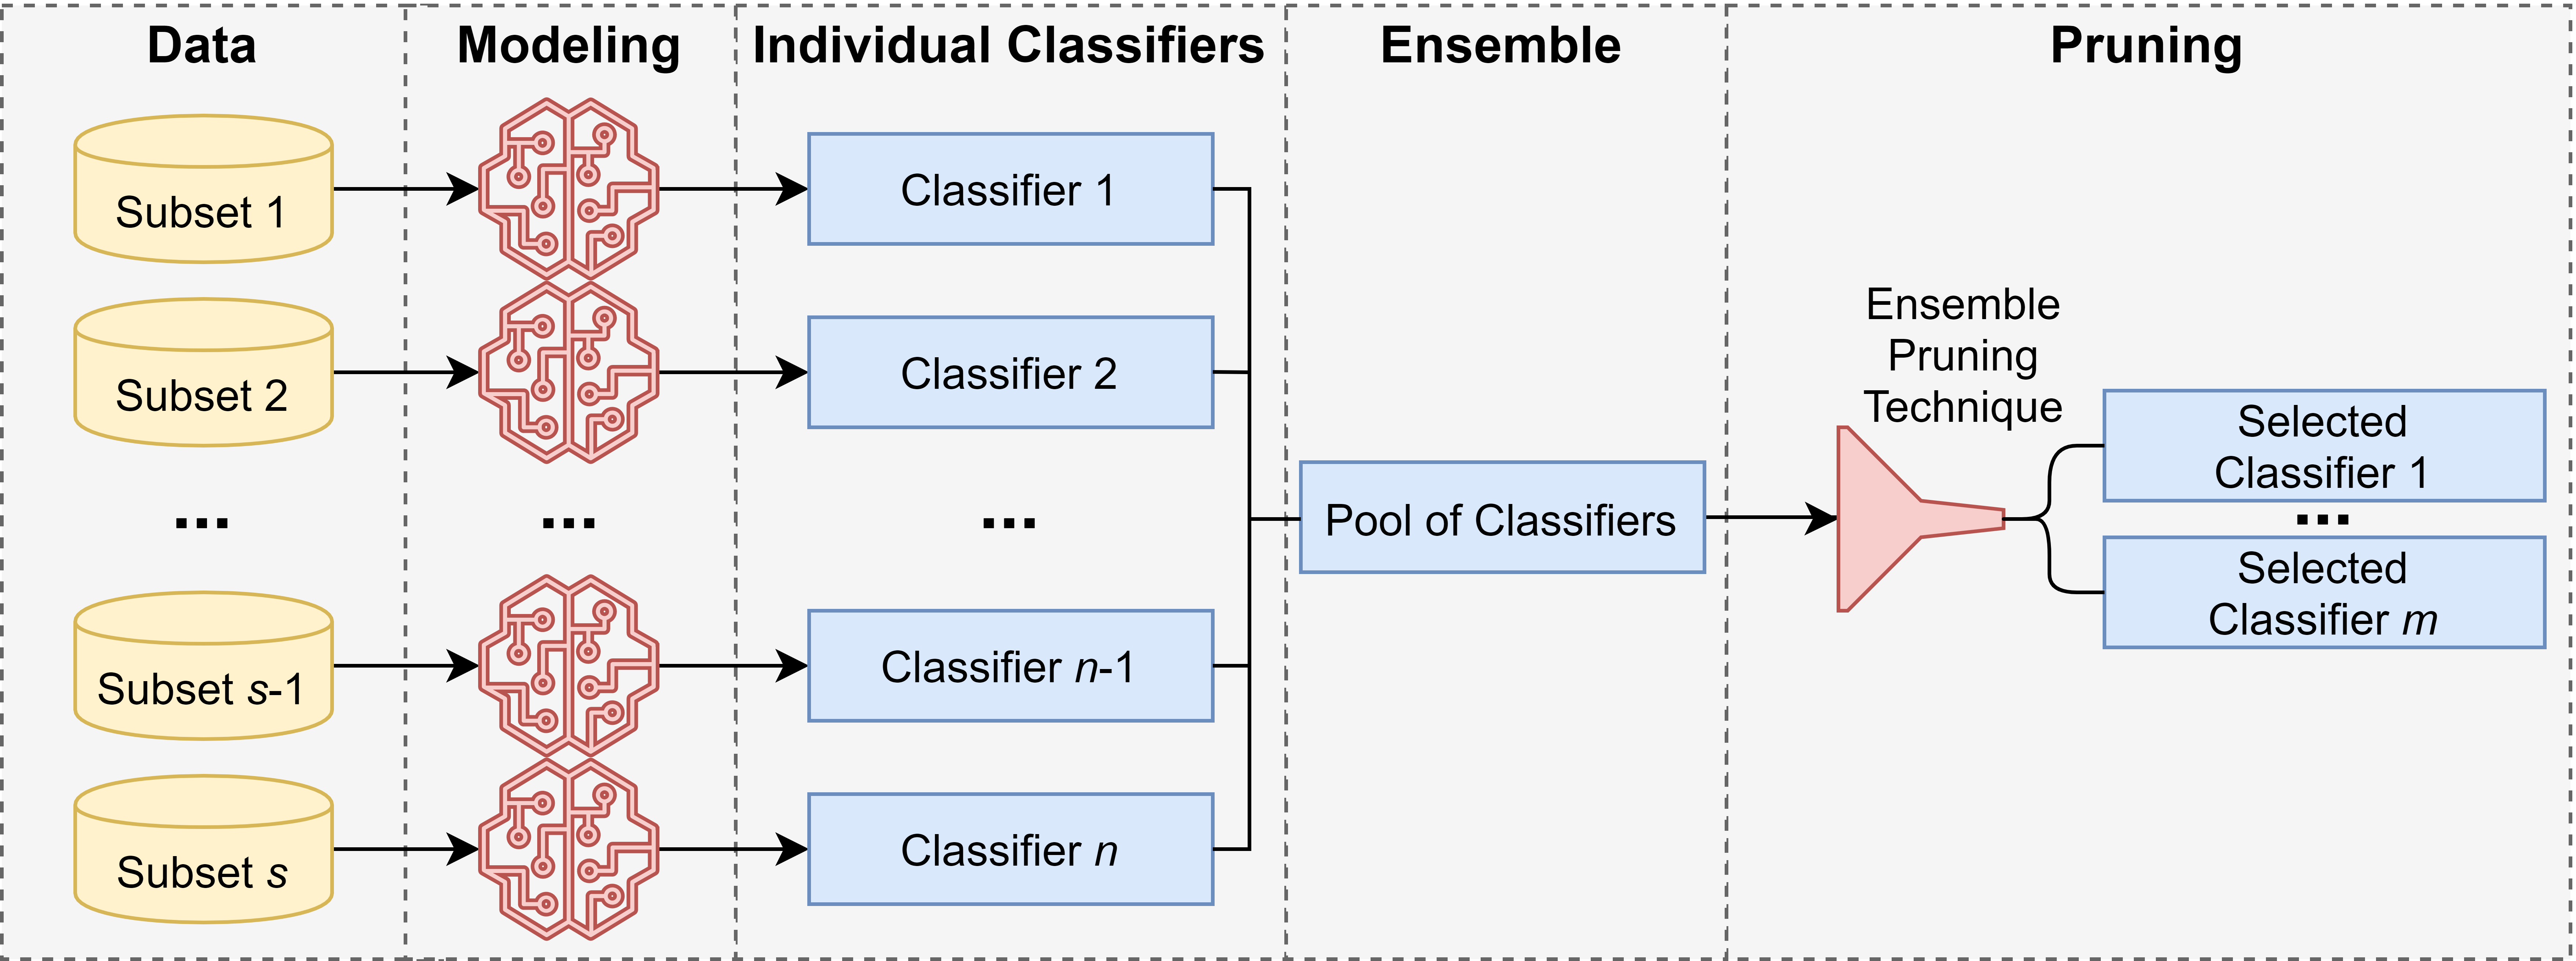
\includegraphics[width=12cm,keepaspectratio]{figs/pruning.png}
\newline \centering{Fonte: Adaptado de \citeonline{cao2018optimizing}.}\label{fig:pruning}
\end{figure}

Analisando a Figura \ref{fig:pruning} é possível observar que diferentes modelos podem ser gerados partindo da mesma amostragem de dados ou mesmo de diferentes \textit{subsets} de forma a criar $n$ classificadores que farão parte do \textit{Ensemble} à depender dos detalhes de cada técnica específica. O \textit{committee} gerado que compreende um \textit{pool} de classificadores é então processado pela técnica escolhida de\textit{ pruning} que irá resultar numa seleção mais adequada de modelos.

O\textit{ pruning} pode ser realizado de diferentes maneiras, conforme apontam \citeonline{martinez2008analysis}, em experimentos para seleção de classificadores utilizando bagging: os métodos ``\textit{Reduce-Error Pruning}'' e ``Kappa \textit{Pruning}'' apresentados por \citeonline{margineantu1997pruning}, os modelos ``\textit{Complementarity Measure}'' e ``\textit{Margin Distance Minimization}'' por \citeonline{martinez2004aggregation} além das técnicas ``\textit{Orientation Ordering}'' por \citeonline{martinez2006pruning} e ``\textit{Boosting-Based Ordering}'' por \citeonline{martinez2007using}.

Experimentos que aplicam\textit{ pruning} em \textit{Ensembles} têm sido empregados com sucesso, como por \citeonline{zhou2002ensembling} aplicado a redes neurais; em \citeonline{hernandez2006pruning} utilizando regressores para bagging; em \citeonline{martinez2008analysis} aplicando\textit{ pruning} também em bagging por meio de ordenações; em \citeonline{chen2009predictive} um modelo baseado em \textit{expected propagation}; em \citeonline{jiang2016novel} baseado em métodos bayesianos; em \citeonline{guo2018margin} por meio da maximização de margens e diversidade de \textit{Ensembles} e em \citeonline{khorashadi2020novel} onde é proposto um modelo baseado em \textit{sparse representation}. 

O exame de qualificação da presente Dissertação de Mestrado foi realizado no dia 18/06/2020 conforme exigências legais do Programa de Pós Graduação em Ciência da Computação. Como sugestão do Membro Avaliador Prof. LD. PhD. João Paulo Papa, a aplicação do método de avaliação da diversidade entre os classificadores (\textit{Diversity Pruning}) poderia trazer incrementos significativos na performance dos \textit{Stackings}, desde as taxas de detecção em si até o tempo de execução. Seguindo tal observação e baseado em \citeonline{herrera2020framework}, os cálculos da diversidade entre os classificadores disponibilizados nas Tabelas \ref{tab:diversidade_bruteforce}, \ref{tab:diversidade_infiltration}, \ref{tab:diversidade_ddos}, \ref{tab:diversidade_portscan}, \ref{tab:diversidade_botnets} e \ref{tab:diversidade_web} foram usados para apresentação dos resultados constantes no Capítulo \ref{result}.


\subsubsection{\textit{Diversity Pruning - Disagreement Measure}}
\label{disagree}


\apudonline{kuncheva2003measures}{herrera2020framework} destacam a possibilidade de se obter um valor $Q$ indicando o quão diferente um classificador $c_1$ é de outro classificador $c_2$ para lidar com um problema de classificação específico. Para tal, é feita uma análise de dois classificadores (\textit{pair-wise}) onde a Equação \ref{eq-disagree} deve ser aplicada: 

\begin{equation}
\label{eq-disagree}
    Q_{c_1,c_2} = \frac{b+c}{a+b+c+d}
\end{equation}

Onde:
\begin{itemize}
    \item $Q$ - Valor de diferença entre os classficadores $c_1$ e $c_2$. Quanto maior, mais diferente. Se $c_1 = c_2$ então $Q = 0$;
    
    \item $c_1$ e $c_2$ - Os dois classificadores escolhidos para a análise \textit{pair-wise};
    
    \item $a$ - Representa o número absoluto de vezes em que tanto $c_1$ quanto $c_2$ realizaram corretamente uma classificação;
    
    \item $b$ - Representa o número absoluto de vezes em que $c_1$ realizou corretamente uma classificação e $c_2$, para os mesmo dados, classificou erroneamente;
    
    \item $c$ - Representa o número absoluto de vezes em que $c_2$ realizou corretamente uma classificação e $c_1$, para os mesmo dados, classificou erroneamente;
    
    \item $d$ - Representa o número absoluto de vezes em que tanto $c_1$ quanto $c_2$ realizaram incorretamente uma classificação;
\end{itemize}

Mais detalhes acerca da implementação da \textit{Disagreement Measure} podem ser encontrados na Seção \ref{modelagem-Stackings}.